\documentclass[hyperref=colorlinks]{beamer}
\mode<presentation>
\usetheme{iclpt}
\setbeamertemplate{navigation symbols}{}
\setbeamertemplate{headline}{
\begin{beamercolorbox}[leftskip=.2cm,rightskip=.2cm,topskip=.2cm,ht=1.1cm,dp=0.1cm,wd=\textwidth]{institute in head/foot}
  
\includegraphics[height=1cm]{icl.pdf}
  \hfill
  
\includegraphics[height=1cm]{../Pics/CMS-Color.pdf}
\end{beamercolorbox}
}
\setbeamertemplate{footline}{
\begin{beamercolorbox}[ht=.55cm,dp=0.4cm,wd=\textwidth,leftskip=.3cm]{author in head/foot}%
  \begin{minipage}[c]{5cm}%
    \usebeamerfont{author in head/foot}
    \insertshortauthor 
    \insertshorttitle
    \end{minipage}\hfill%
  \insertframenumber{} / \pageref{lastframe}
  \hfill
  \begin{minipage}{6cm}
    \hfill
  \end{minipage}
\end{beamercolorbox}%
}

\usepackage{color}
\usepackage{tabularx,colortbl}
\usepackage{graphicx}
\usepackage{pdfpages}
\usepackage{feynmp}
\usepackage{tikz}
\usetikzlibrary{calc, shapes, backgrounds,arrows,positioning}
\DeclareGraphicsRule{*}{mps}{*}{}

\title{\vspace{-0.2cm} VBF Higgs to Invisible}
\subtitle{\vspace{-0.7cm}}
\author[]{}%\underline{P. Dunne}} % A.M. Magnan and A. Nikitenko Joao Pela with \\ R. Aggleton, J. Brooke: Bristol \\ C.Asawangtrakuldee, Q.Li: Peking \\ P. Srimanobhas: Chulalongkorn \\ S. Kumar, K. Mazumdar: Mumbai}
\titlegraphic{
  \vspace{-0.7cm}
  %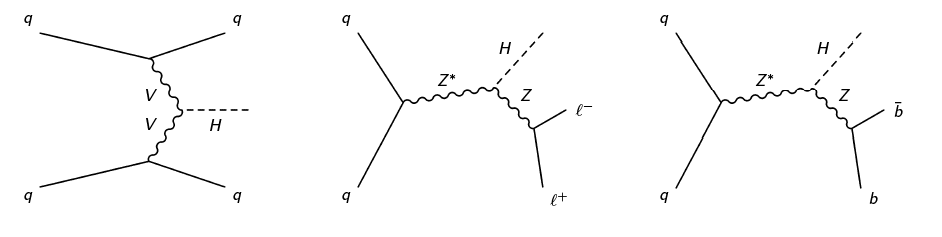
\includegraphics[width=\textwidth]{TalkPics/invcomb021213/feyndiags}
  %% \begin{fmfgraph*}(100,70)
  %%         \fmfleft{i1,i2}
  %%         \fmfright{o1,o2,o3}
  %%         \fmf{fermion}{i1,v1,o1}
  %%         \fmf{fermion}{i2,v2,o3}
  %%         \fmf{phantom,tension=4/5}{v1,v2}
  %%         \fmffreeze
  %%         \fmf{photon,label=$W,,Z$}{v1,v3}
  %%         \fmf{photon,label=$W,,Z$}{v2,v3}
  %%         \fmf{dashes}{v3,o2}
  %%         \fmflabel{$q$}{i1}
  %%         \fmflabel{$q$}{i2}
  %%         \fmflabel{$q$}{o1}
  %%         \fmflabel{$q$}{o3}
  %%         \fmflabel{$H$}{o2}
  %%       \end{fmfgraph*}
}
\date{}
\begin{document}
\begin{fmffile}{higgsexoupdatefeyndiags}
\tikzstyle{every picture}+=[remember picture]

%TITLE PAGE
\section{Title}
\begin{frame}
  \titlepage
  
\end{frame}

\begin{frame}
  \frametitle{W MC}
  \begin{block}{Run 1 Reminder}
    \begin{itemize}
    \item In run 1 we split $W\rightarrow\ell\nu$ samples by lepton at generator level
    \item $W\rightarrow\tau\nu$ events were classified according to $\tau$ decay:
    \item[-] e.g. $W\rightarrow\tau\nu\rightarrow\mu\nu\nu\nu$ put in muon category etc.
    \item Done by checking for status 3 lepton
    \end{itemize}
  \end{block}
  \begin{block}{Run 2}
    \begin{itemize}
    \item No more status 3, approximately replaced by status 21-29
    \item In some cases status 21-29 particle replaced by status 1 or 2      
    \end{itemize}
    \end{block}
\end{frame}

\begin{frame}
  \frametitle{W MC: replacing status 3}
  \begin{block}{New strategy}
    \begin{itemize}
    \item Use list of W daughters to find lepton flavour
    \item If a $\tau$ is found check its daughters to determine $\tau$ decay
    \item[-] $\tau$ often radiates, need to check recursively until a decay is found
    \end{itemize}
  \end{block}
  \begin{block}{}
    \begin{itemize}
    \item Since yesterday bug identified, correctly classifies all events light trees made
    \end{itemize}
  \end{block}
\end{frame}


\begin{frame}
  \frametitle{W Comparison}
  \begin{block}{}
    \begin{itemize}
    \item As recommended weights now removed to make it clearer if difference is from gen/reconstruction
    \item Distributions still normalised to 1
    \item Same set of plots as for QCD and signal included for reference
    \item Selection as for QCD is: $\eta_{j1} \cdot \eta_{j2}<0,\, \eta_{j1}<4.7,\, \eta_{j2}<4.7,$
      $p_{T}^{\text{j1}}>50 \,\text{GeV},\,p_{T}^{\text{j2}}>40\,\text{GeV},$
      $\Delta\eta_{jj}>3.6,\, M_{jj}>800\,\text{GeV},$
      $MET>90\,\text{GeV},$
      $METsig>3.$]
    \item As met significance is a different variable in runs 1 and 2 this may bias comparison
    \item Additionally to above cuts enu, munu and taunu categories applied
    \end{itemize}
  \end{block}
\end{frame}

\begin{frame}
  \frametitle{W enu Comparison: run 1 vs run 2: Jet $p_{T}$}
  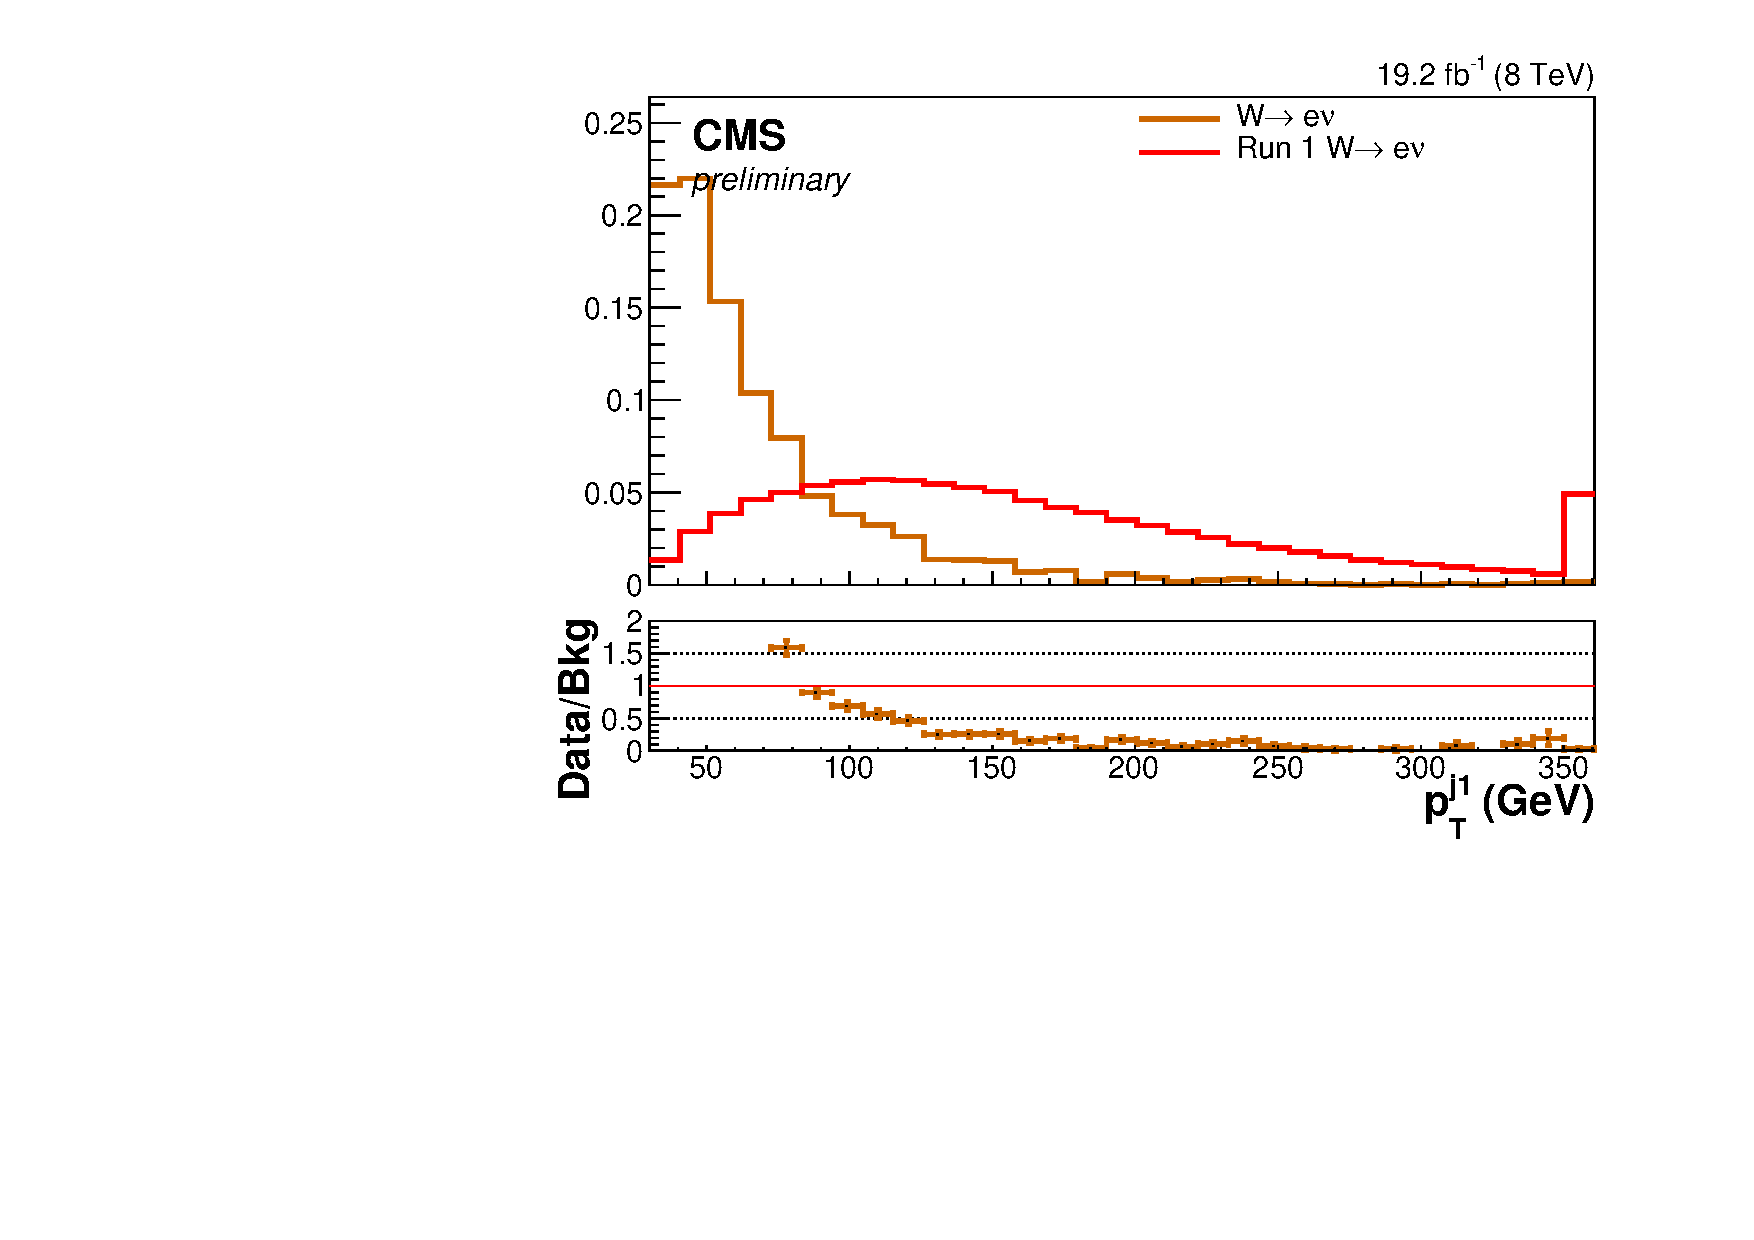
\includegraphics[width=.5\textwidth]{TalkPics/wcontplots090615/output_run1compdynoweight/enu_norm_jet1_pt.pdf}
  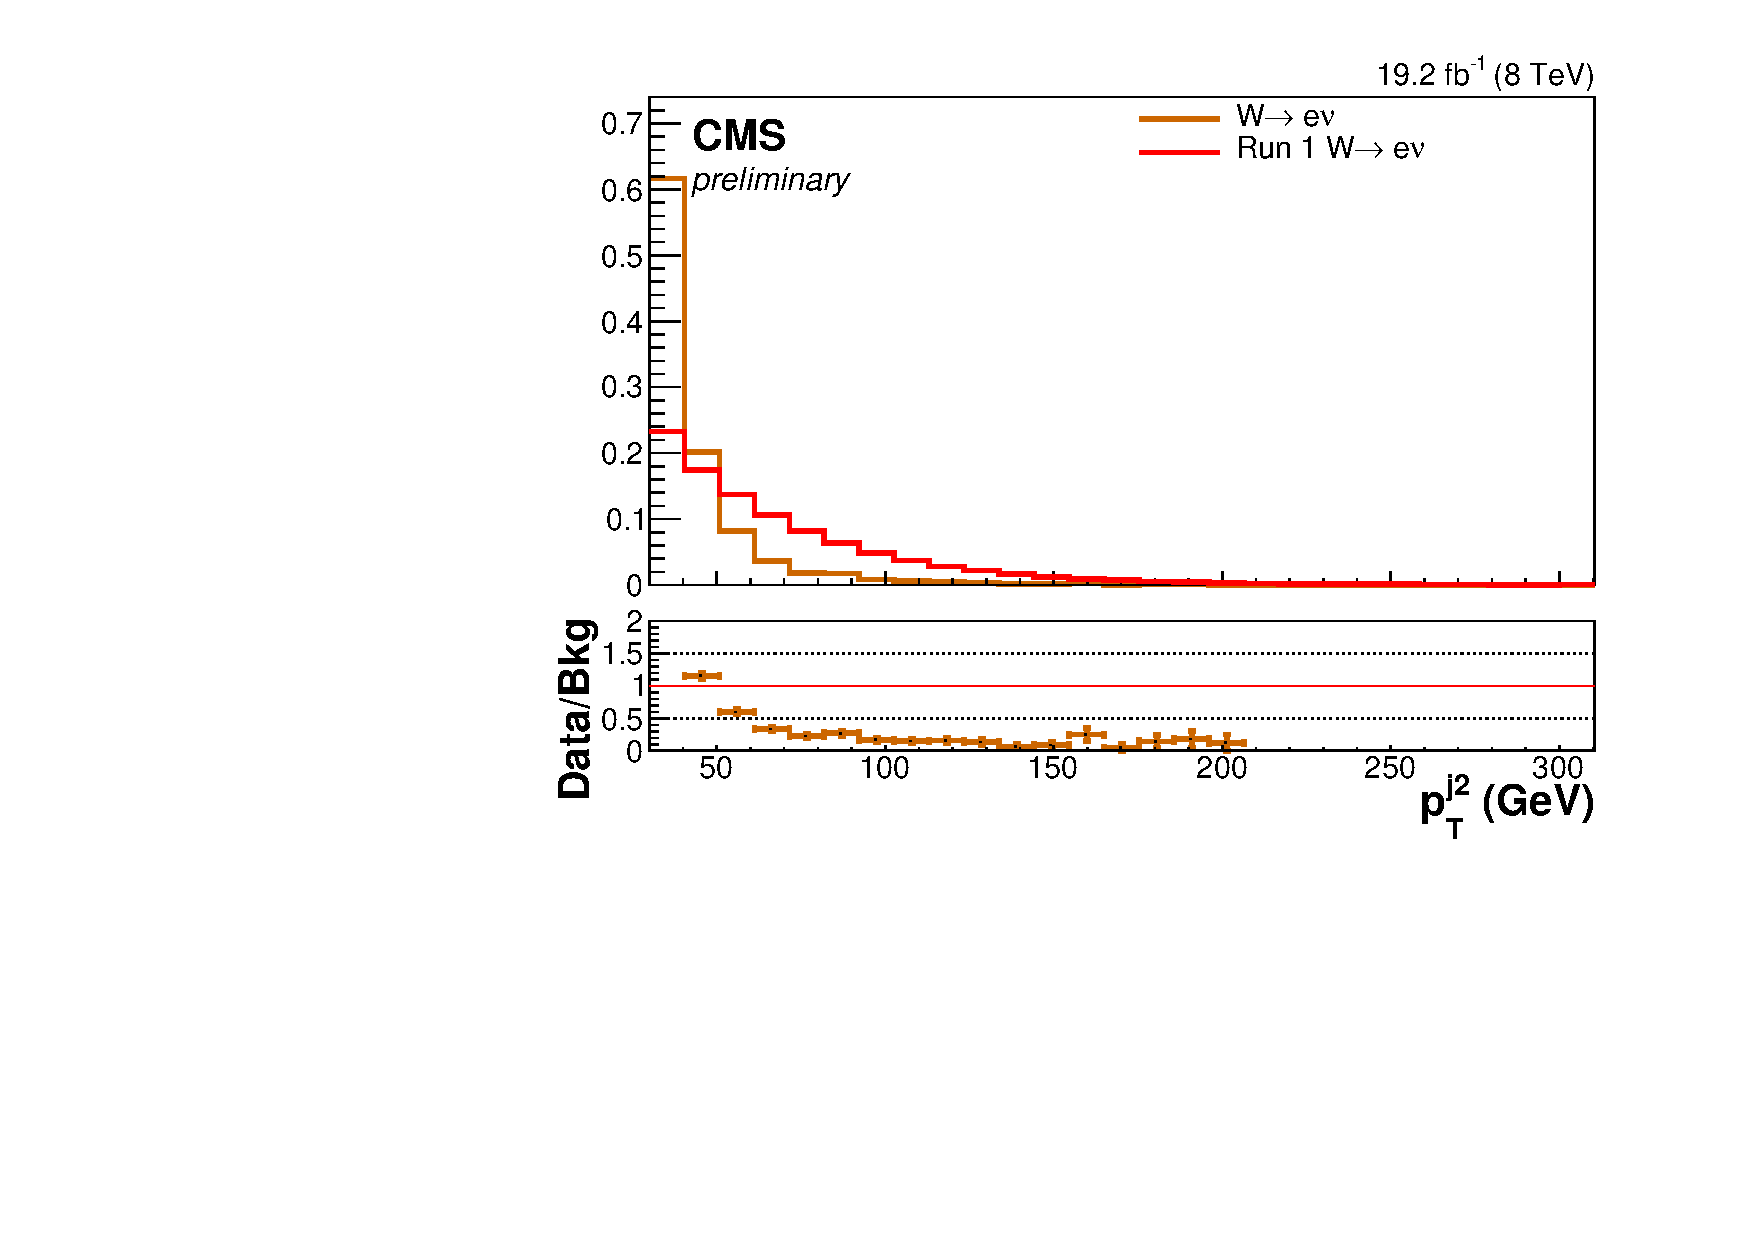
\includegraphics[width=.5\textwidth]{TalkPics/wcontplots090615/output_run1compdynoweight/enu_norm_jet2_pt.pdf}
  \begin{block}{}
    \begin{itemize}
    \item[-] Run 2 much lower could be due to met significance cut bias
    \end{itemize}
  \end{block}
\end{frame}

\begin{frame}
  \frametitle{W enu Comparison: run 1 vs run 2: Jet $\eta$}
  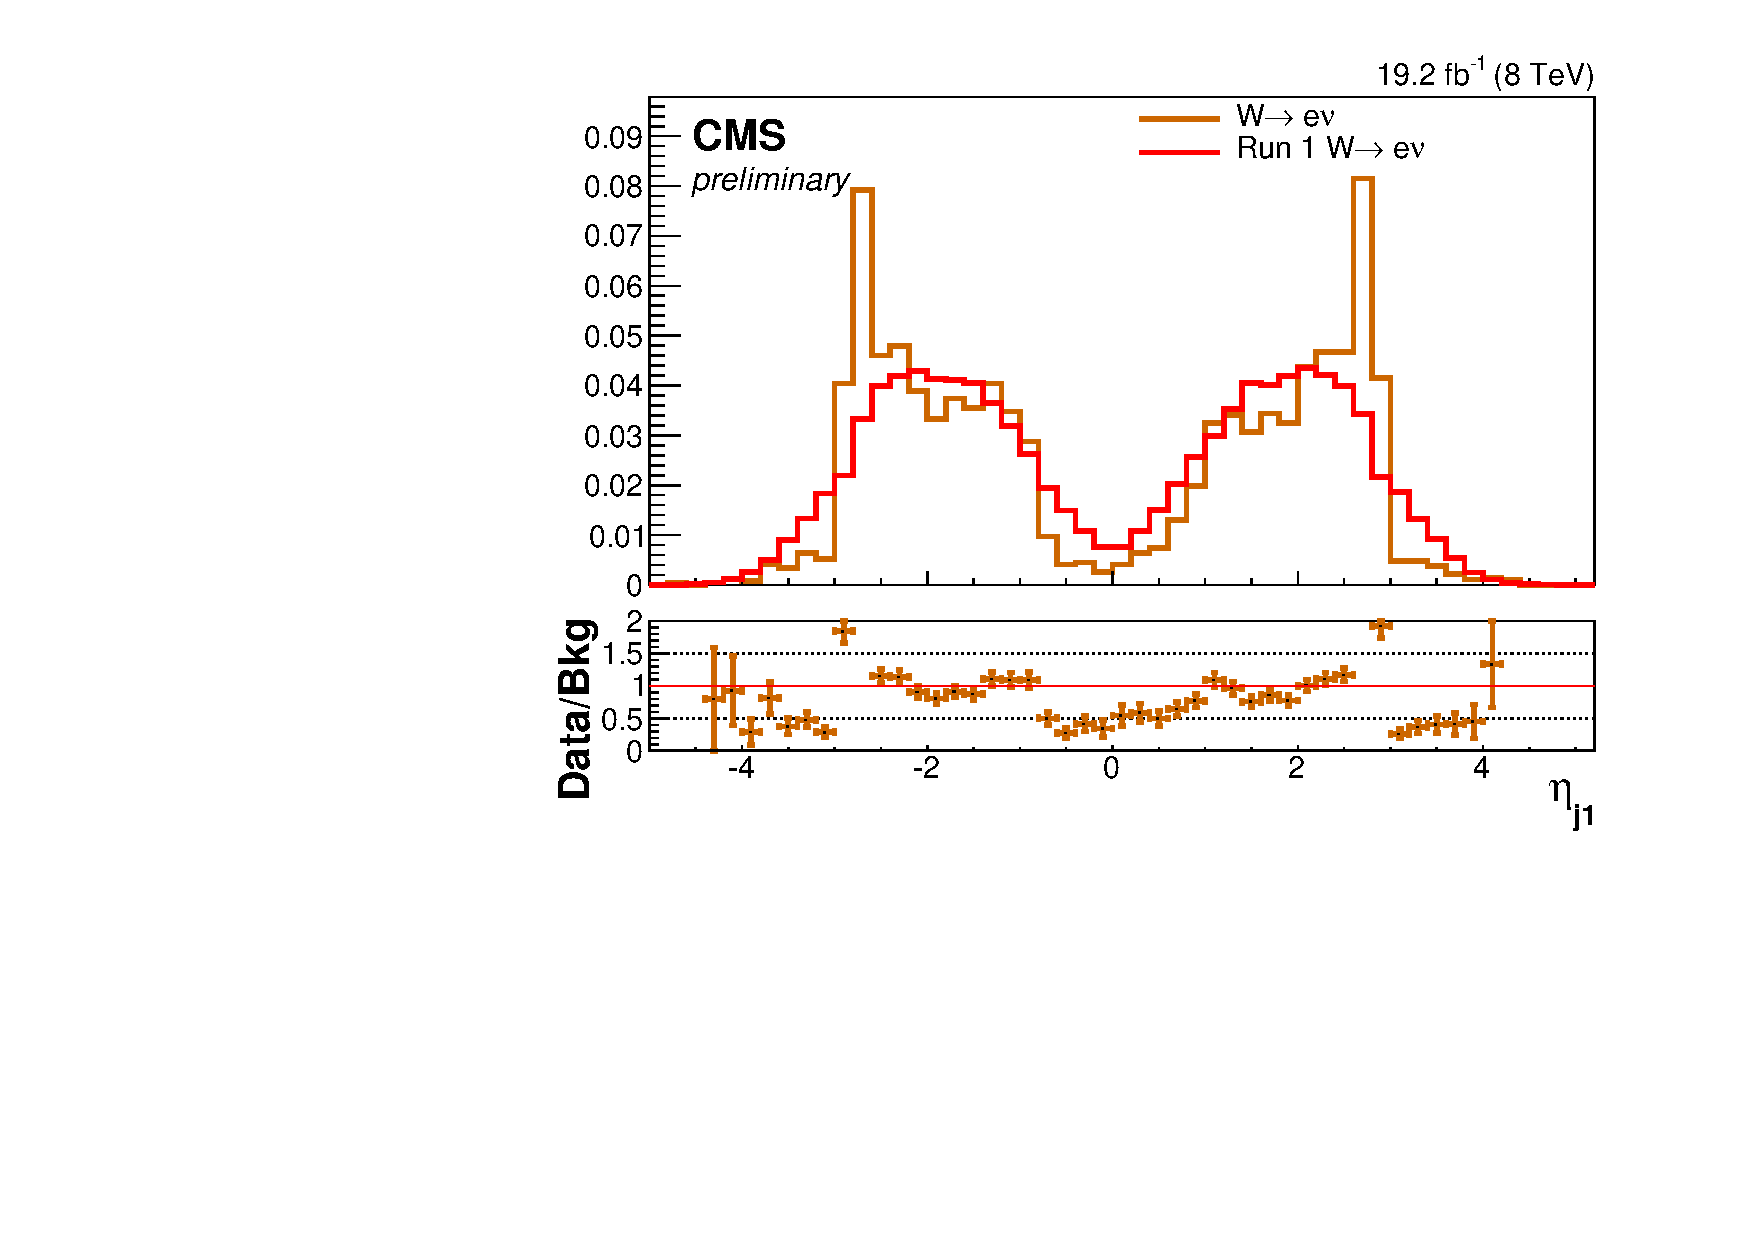
\includegraphics[width=.5\textwidth]{TalkPics/wcontplots090615/output_run1compdynoweight/enu_norm_jet1_eta.pdf}
  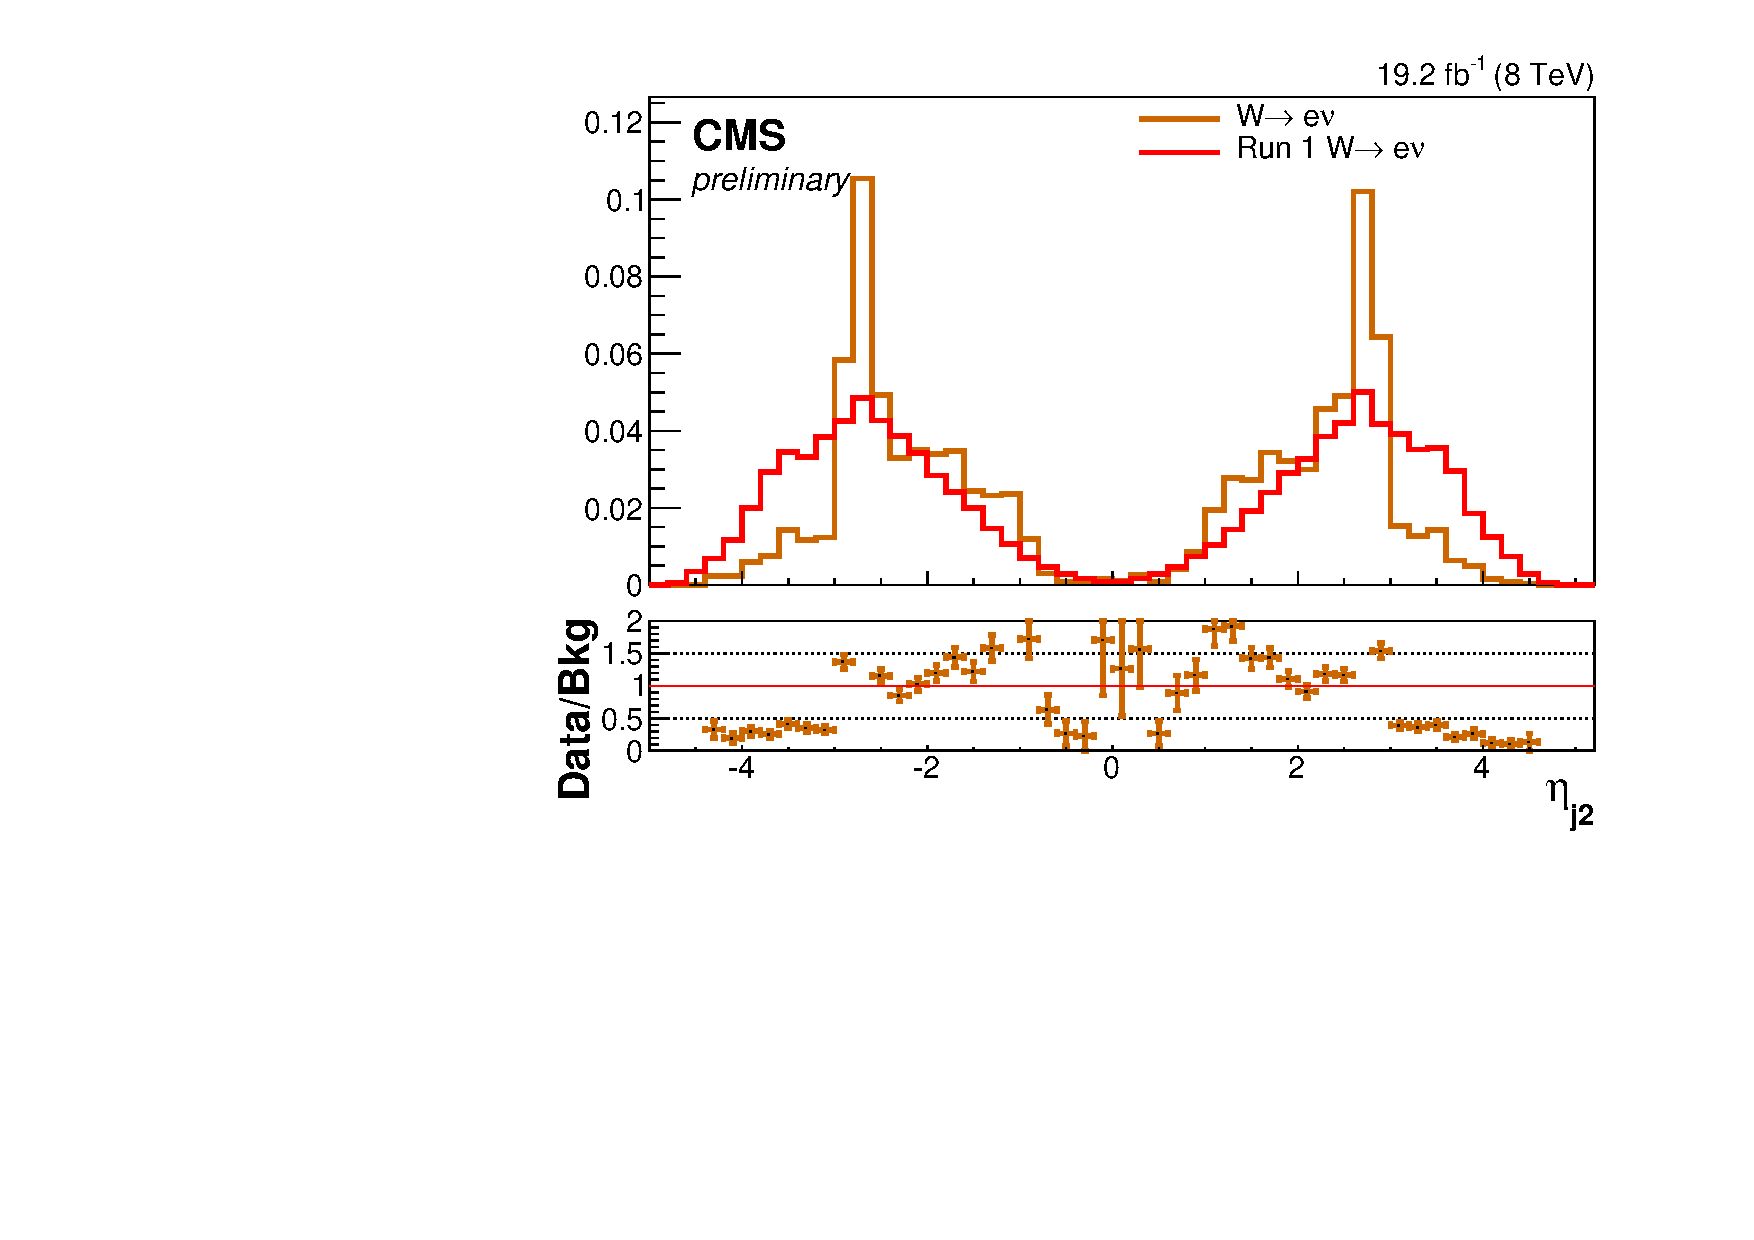
\includegraphics[width=.5\textwidth]{TalkPics/wcontplots090615/output_run1compdynoweight/enu_norm_jet2_eta.pdf}
  \begin{block}{}
    \begin{itemize}
    \item Ears still apparent
    \end{itemize}
  \end{block}
\end{frame}

\begin{frame}
  \frametitle{W enu Comparison: run 1 vs run 2: Jet $\phi$}
  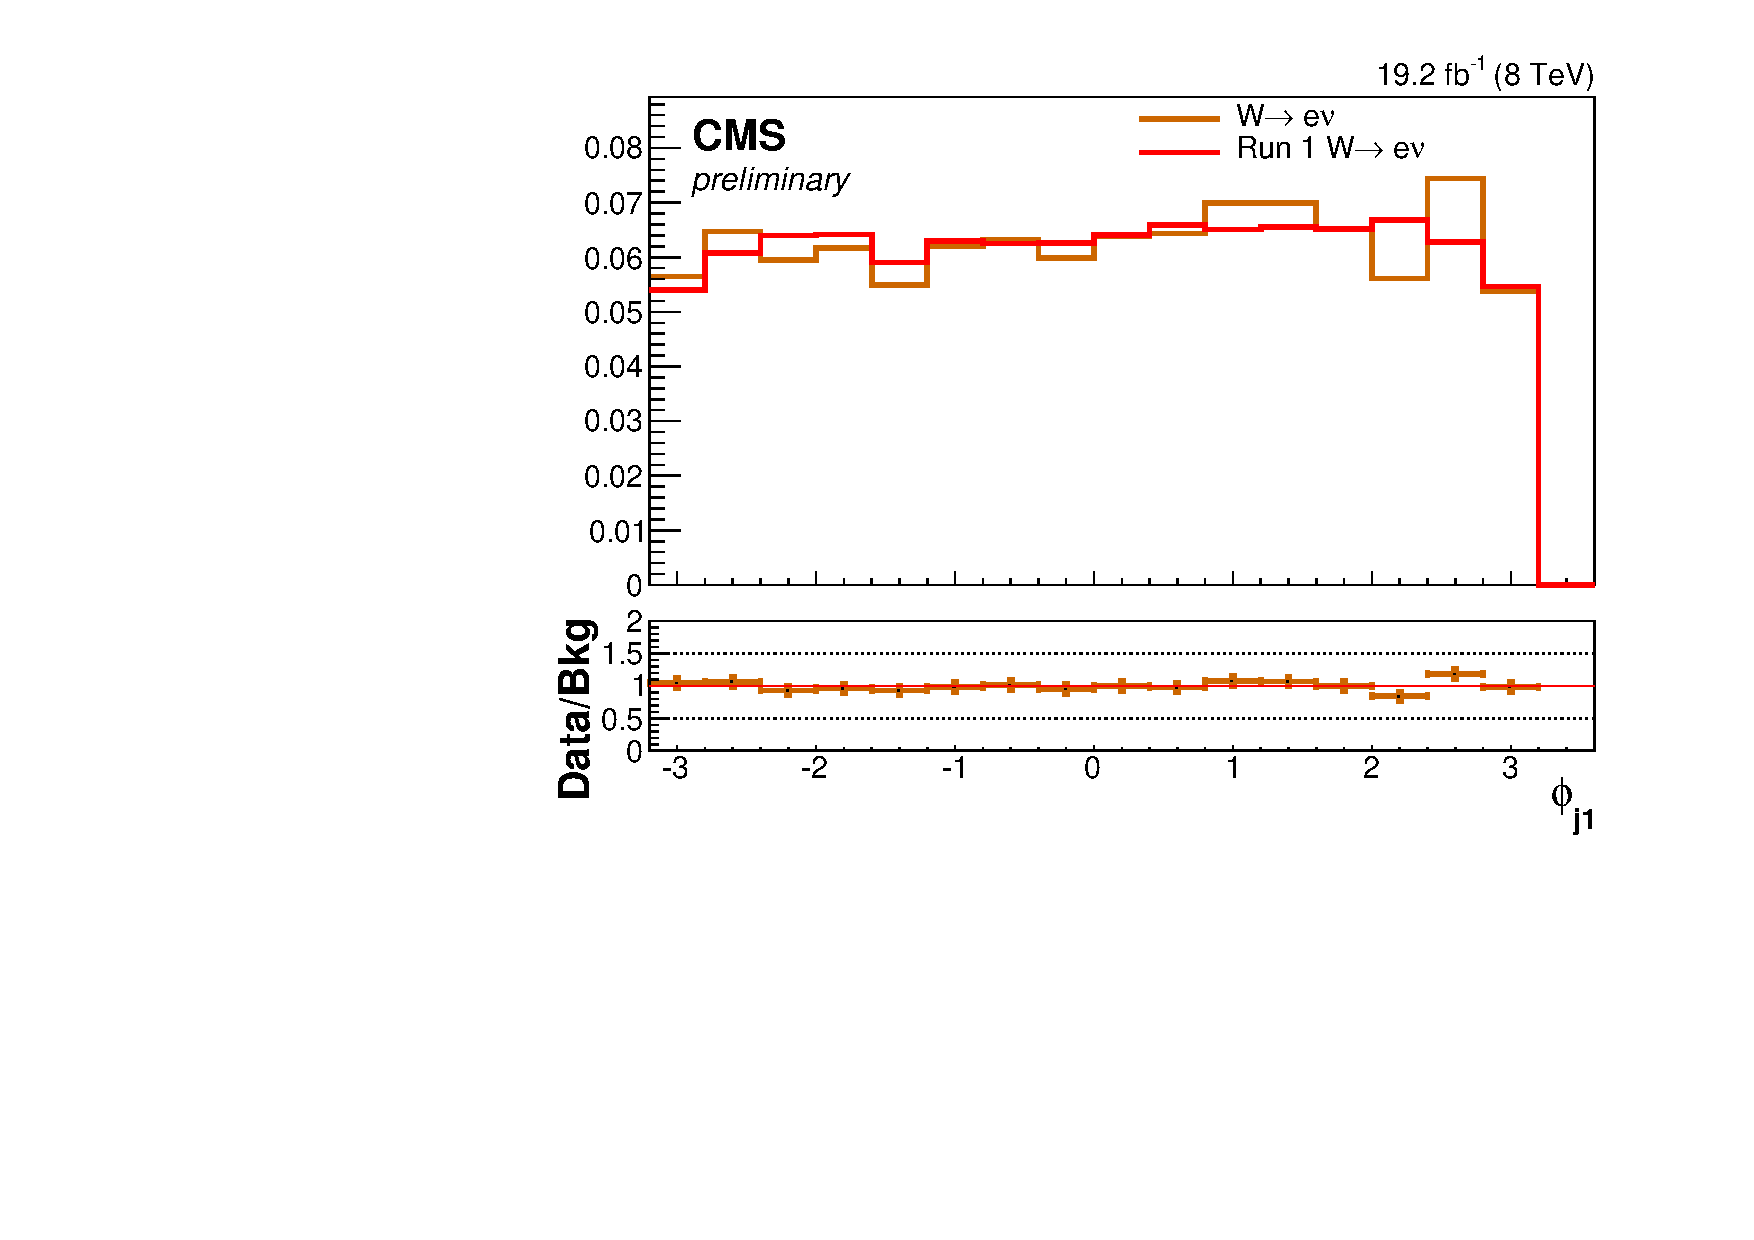
\includegraphics[width=.5\textwidth]{TalkPics/wcontplots090615/output_run1compdynoweight/enu_norm_jet1_phi.pdf}
  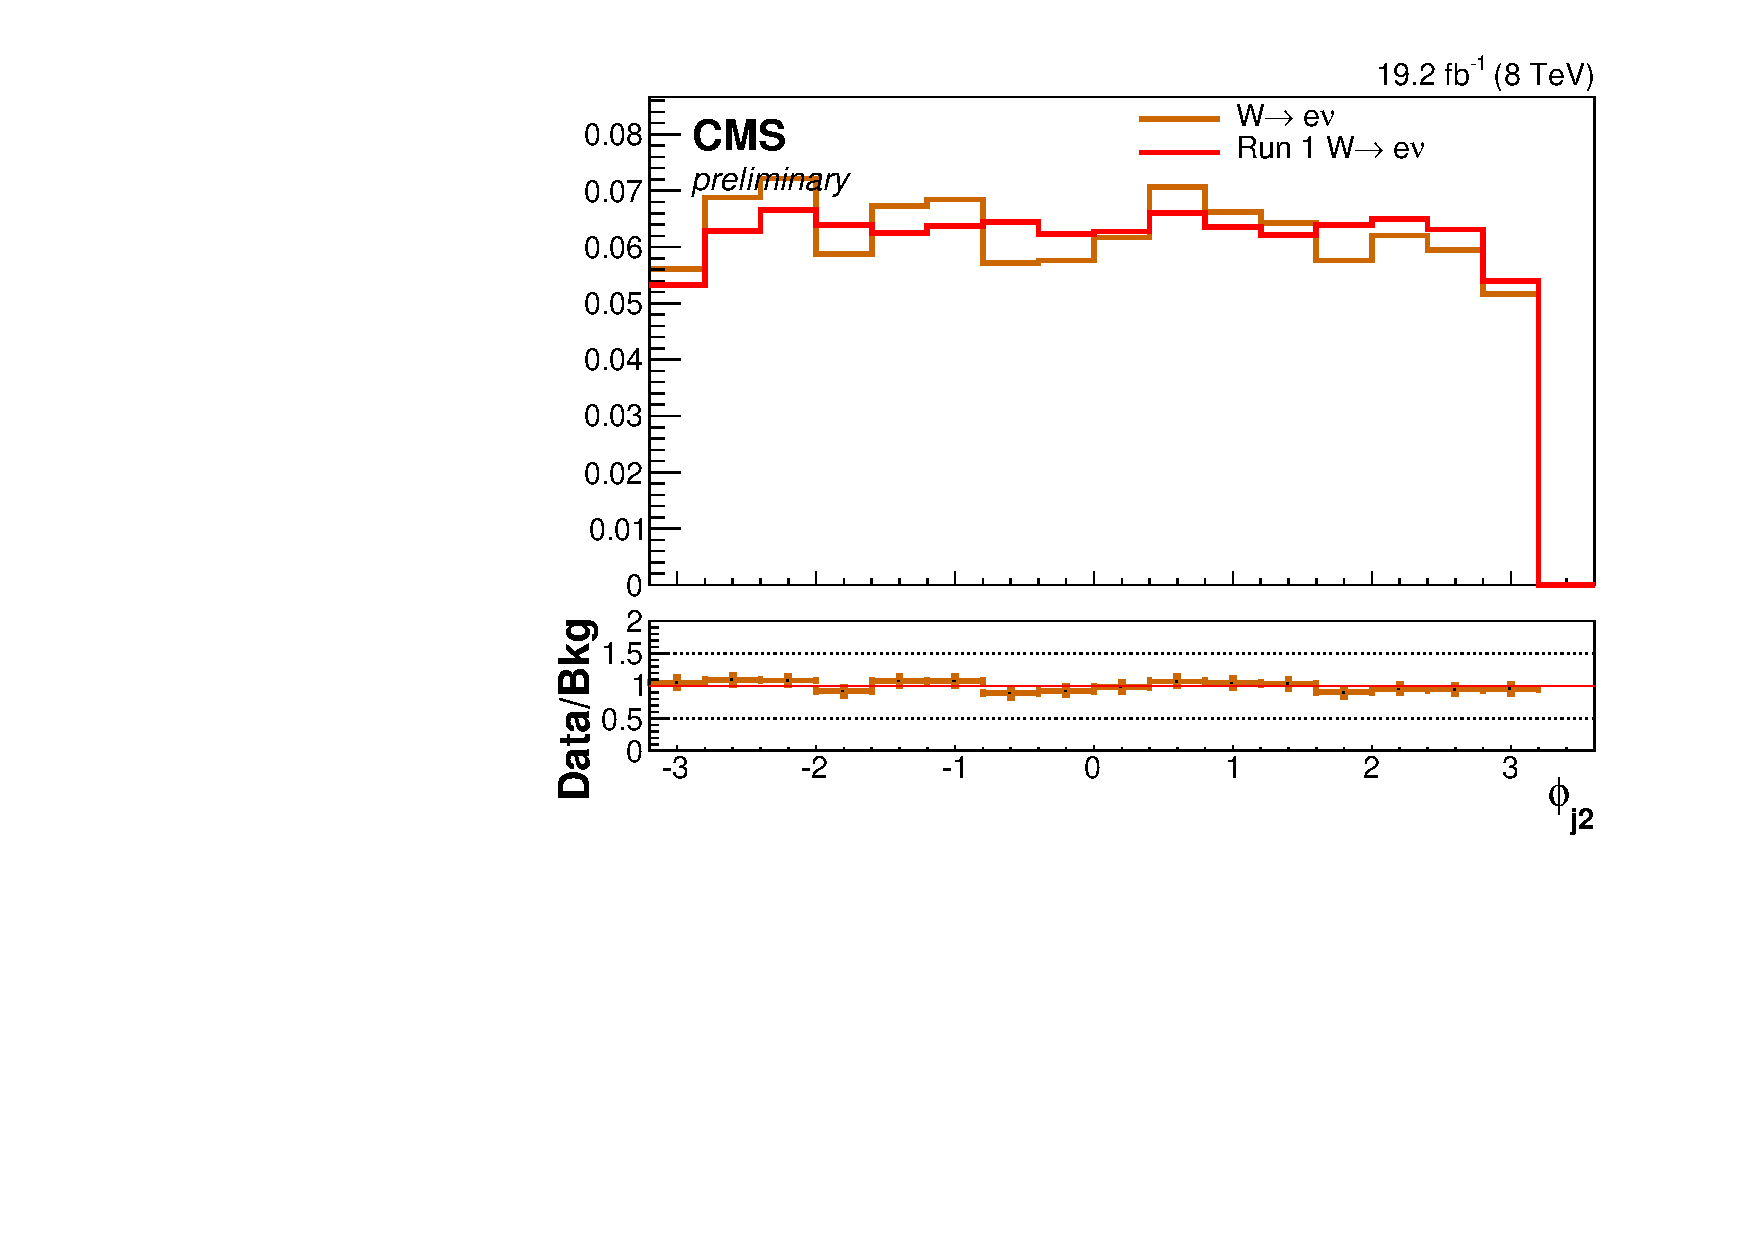
\includegraphics[width=.5\textwidth]{TalkPics/wcontplots090615/output_run1compdynoweight/enu_norm_jet2_phi.pdf}
  \begin{block}{}
    \begin{itemize}
    \item $\phi$ distributions look similar within stat error
    \end{itemize}
  \end{block}
\end{frame}

\begin{frame}
  \frametitle{W enu Comparison: run 1 vs run 2: Met}
  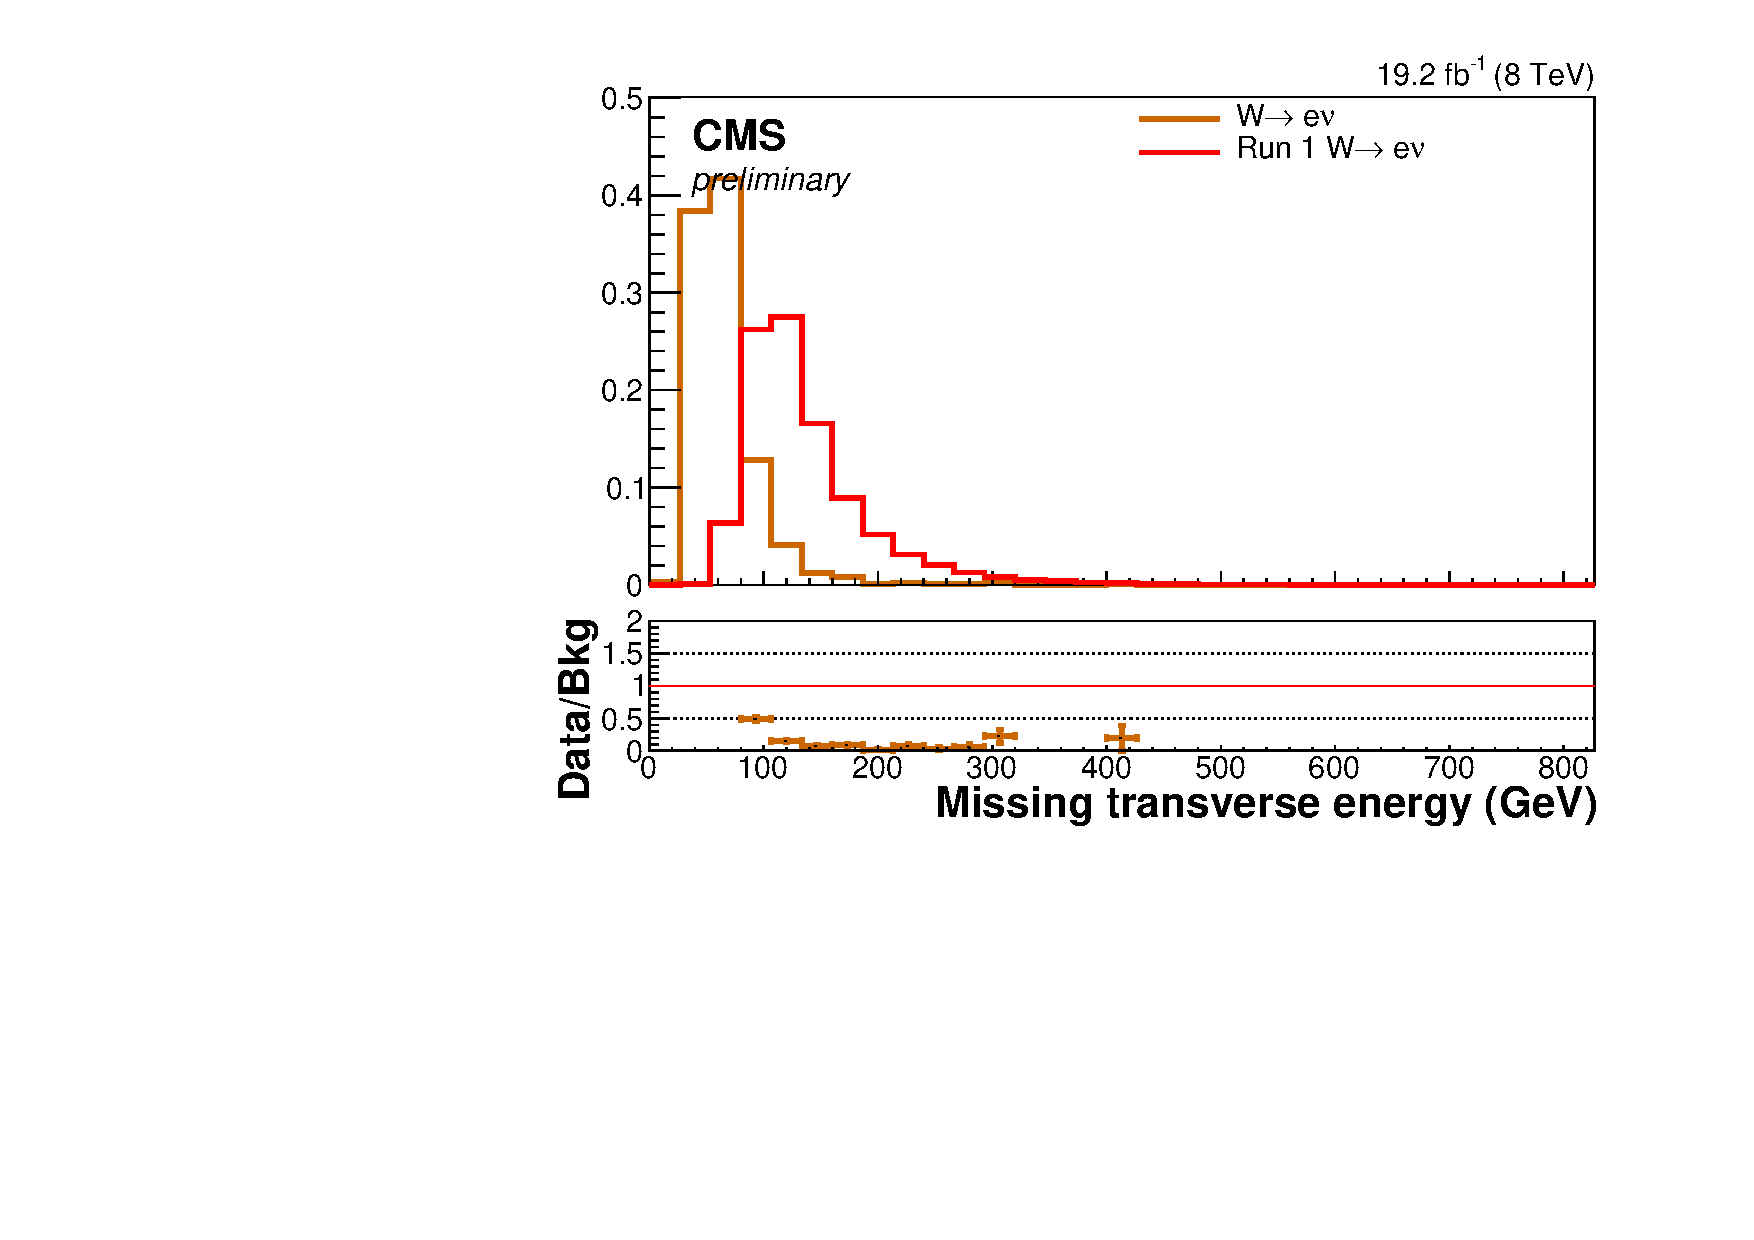
\includegraphics[width=.5\textwidth]{TalkPics/wcontplots090615/output_run1compdynoweight/enu_norm_metnomuons.pdf}
  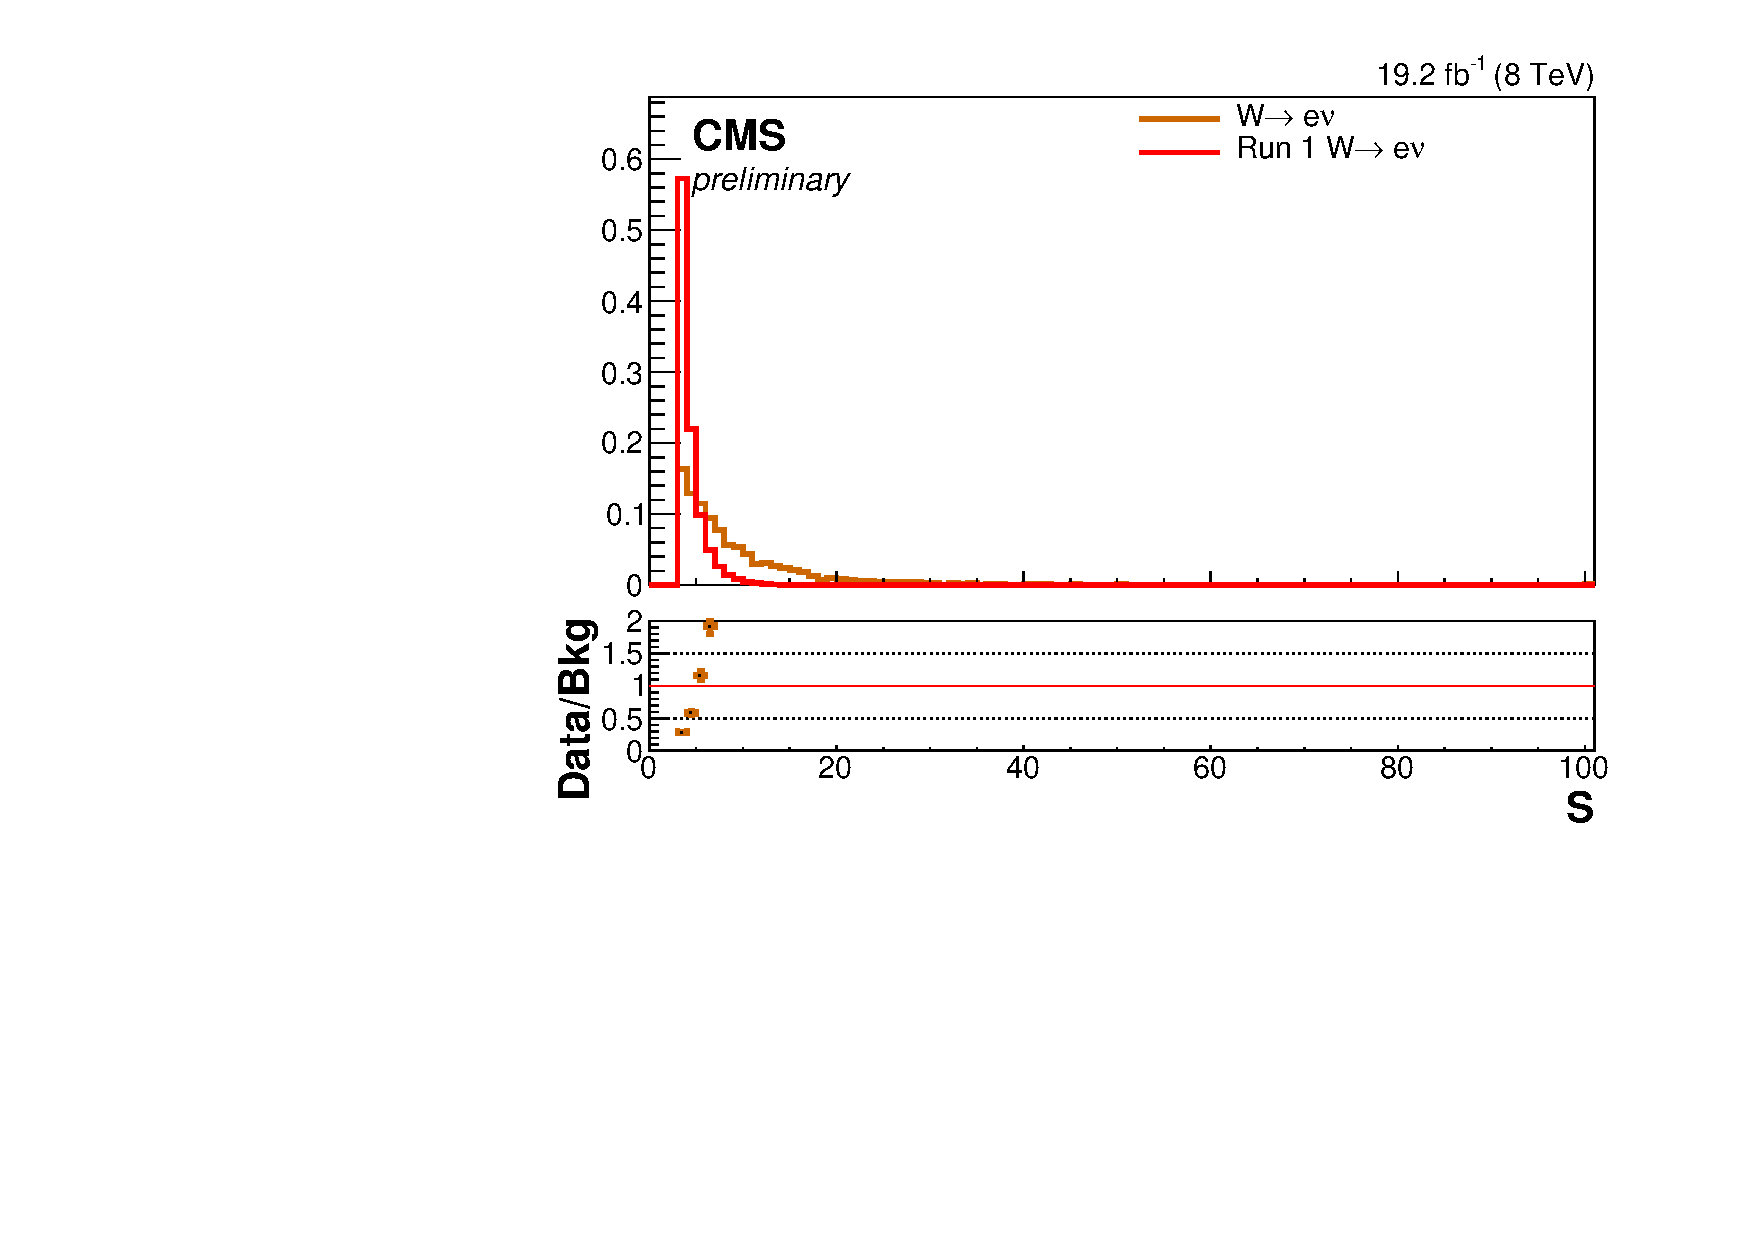
\includegraphics[width=.5\textwidth]{TalkPics/wcontplots090615/output_run1compdynoweight/enu_norm_metnomu_significance.pdf}
  \begin{block}{}
    \begin{itemize}
    \item Metnomu lower for run 2
    \item Met significance is a different variable in miniAOD to the one we used in run 1
    \end{itemize}
  \end{block}
\end{frame}

\begin{frame}
  \frametitle{W enu Comparison: run 1 vs run 2: $\Delta\phi$ variables}
  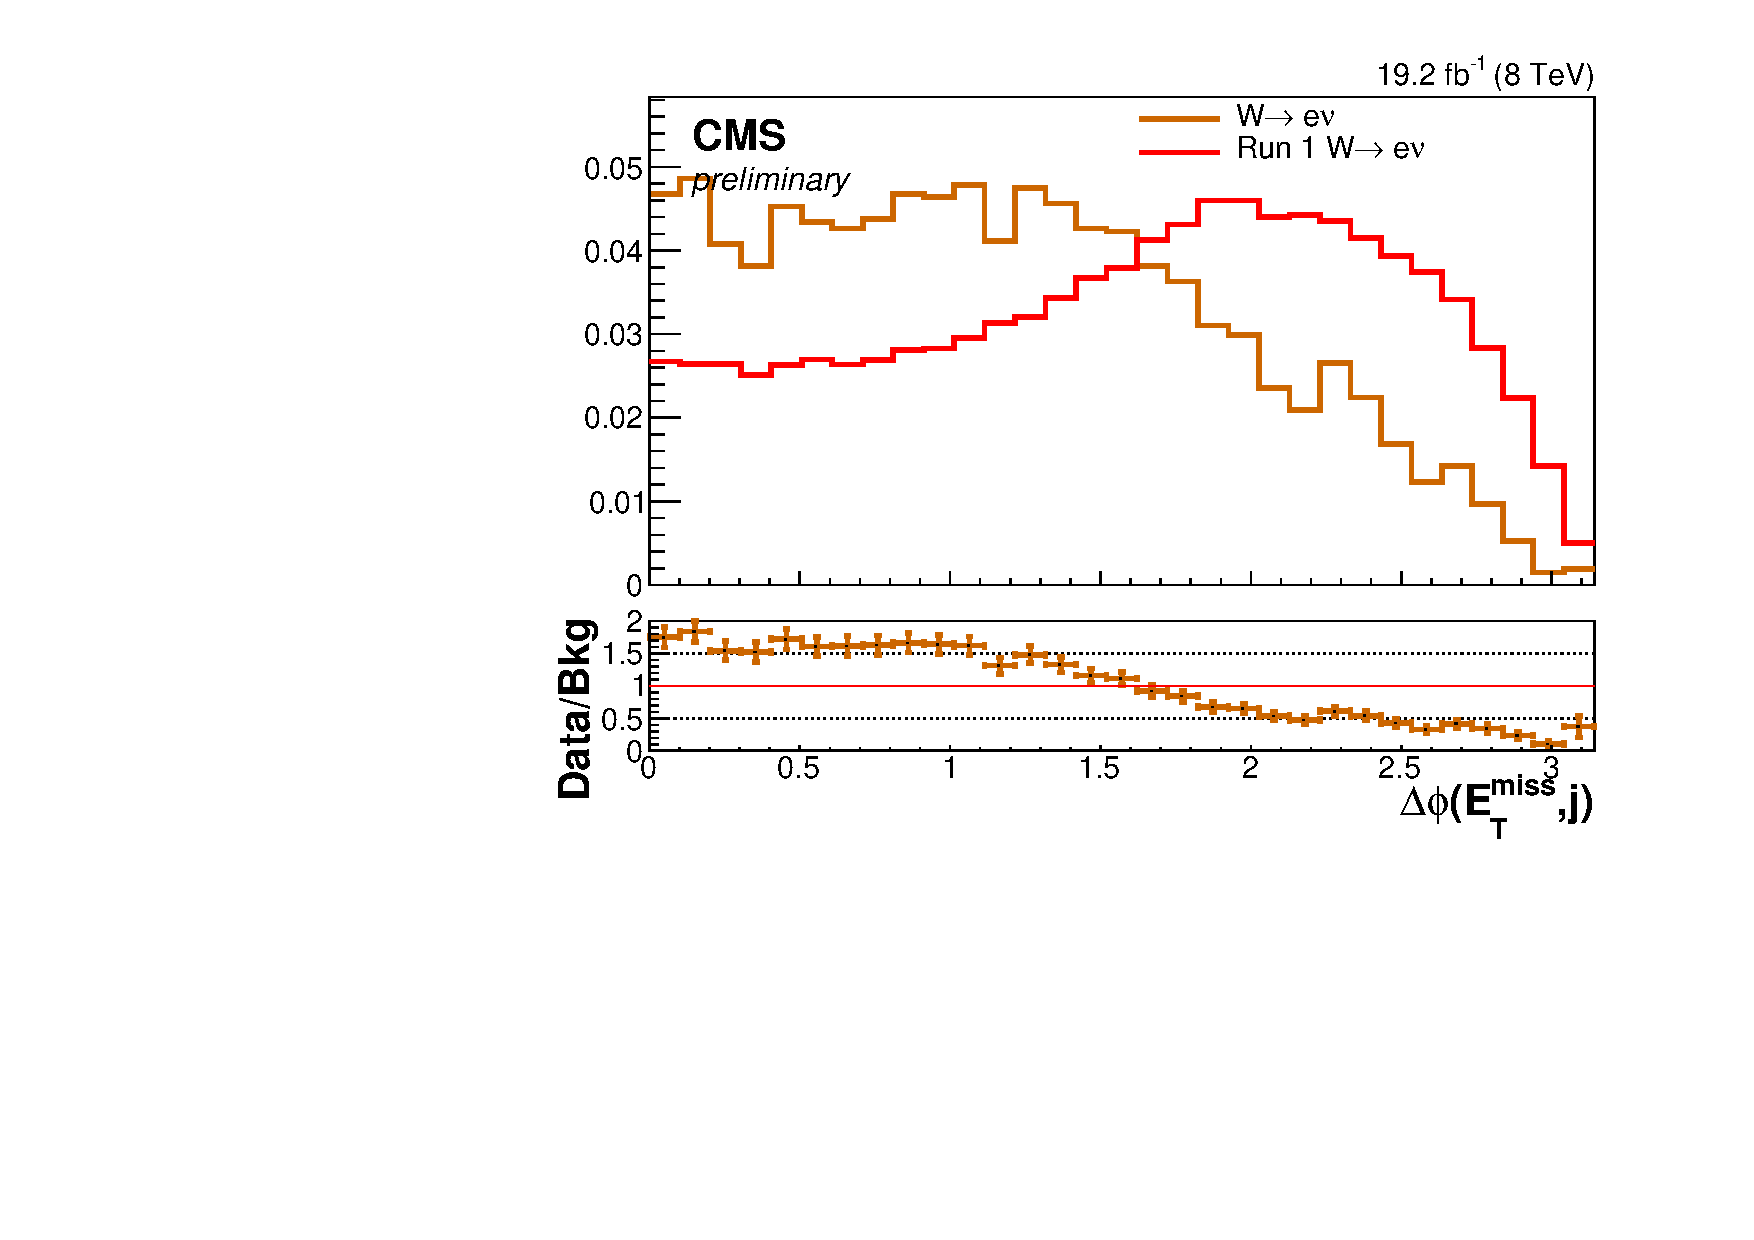
\includegraphics[width=.5\textwidth]{TalkPics/wcontplots090615/output_run1compdynoweight/enu_norm_alljetsmetnomu_mindphi.pdf}
  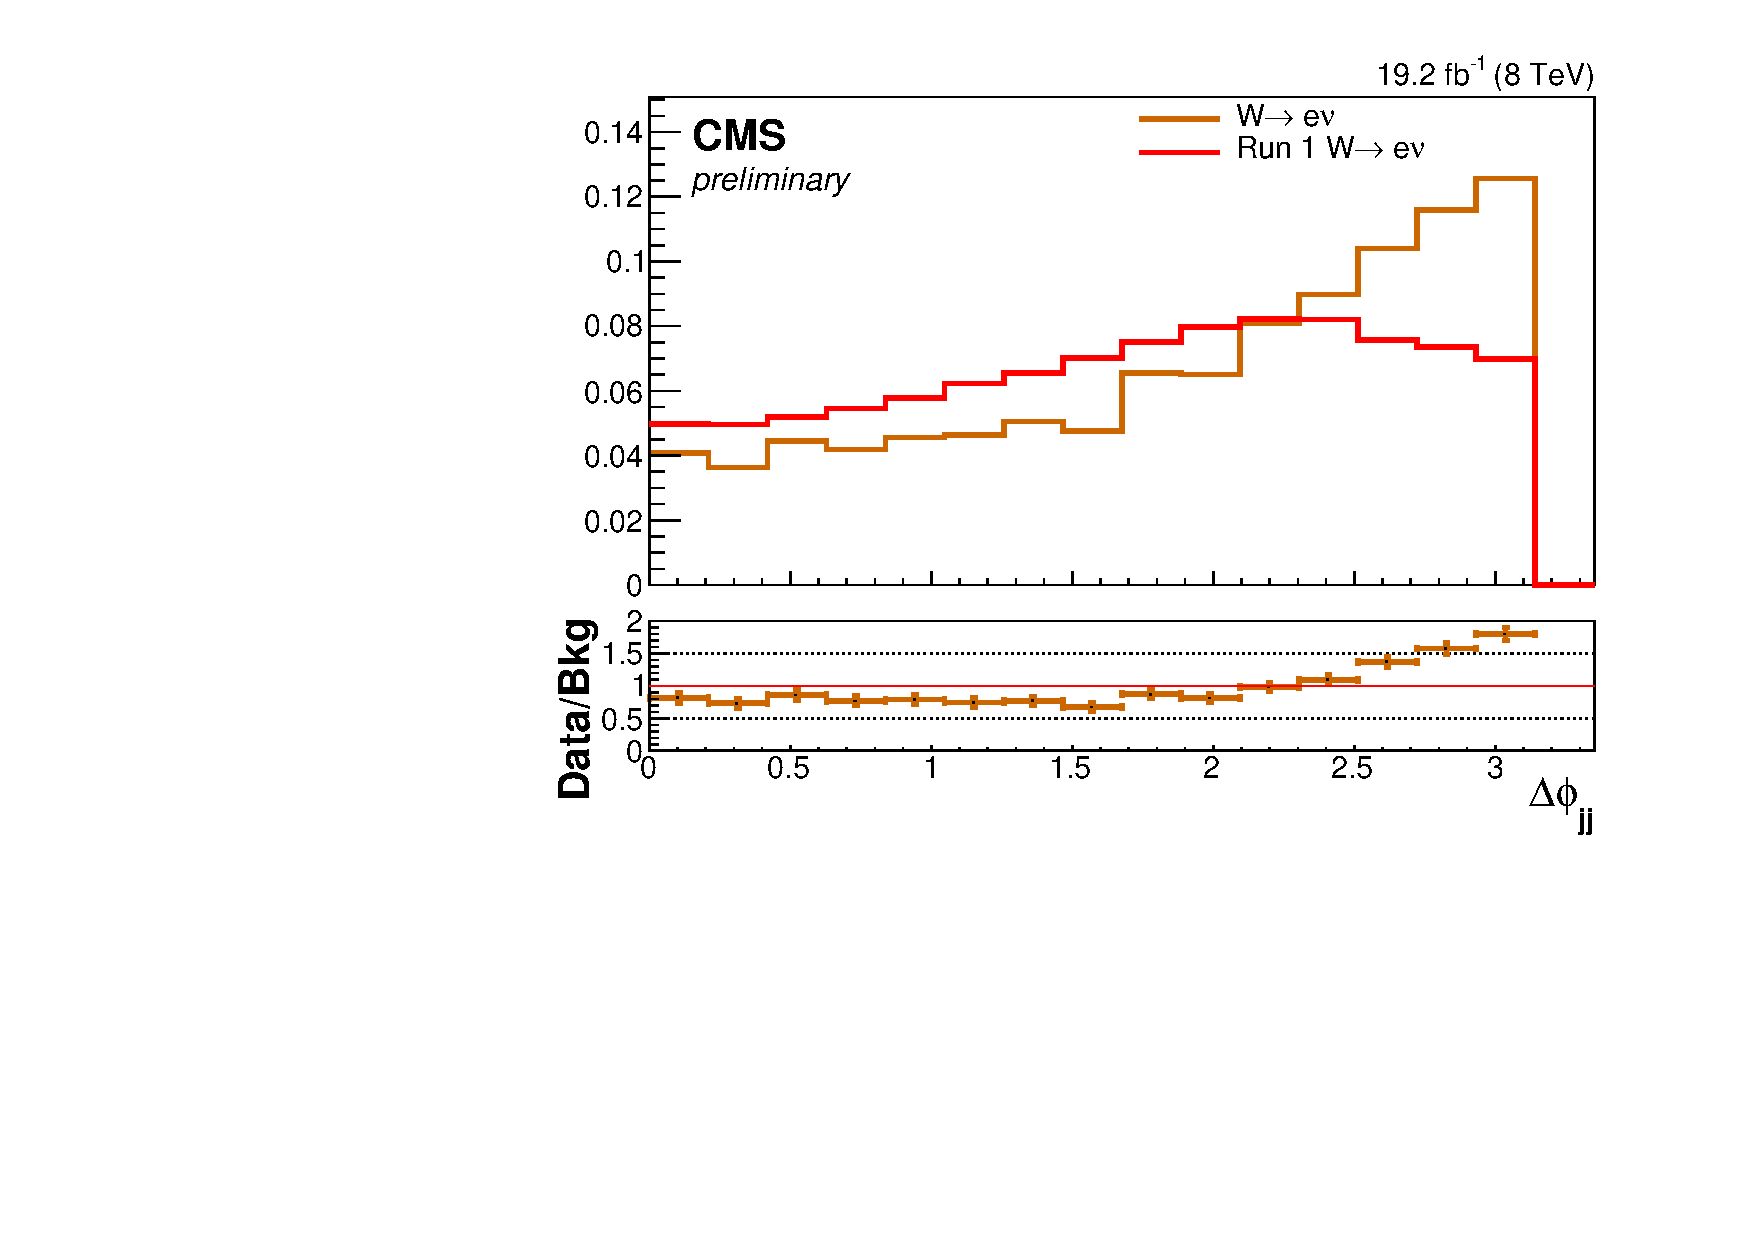
\includegraphics[width=.5\textwidth]{TalkPics/wcontplots090615/output_run1compdynoweight/enu_norm_dijet_dphi.pdf}
  \begin{block}{}
    \begin{itemize}
    \item Much more background like for run 2
    \item[-] could be due to met significance cut bias
    \end{itemize}
  \end{block}
\end{frame}

\begin{frame}
  \frametitle{W enu Comparison: run 1 vs run 2: dijet variables}
  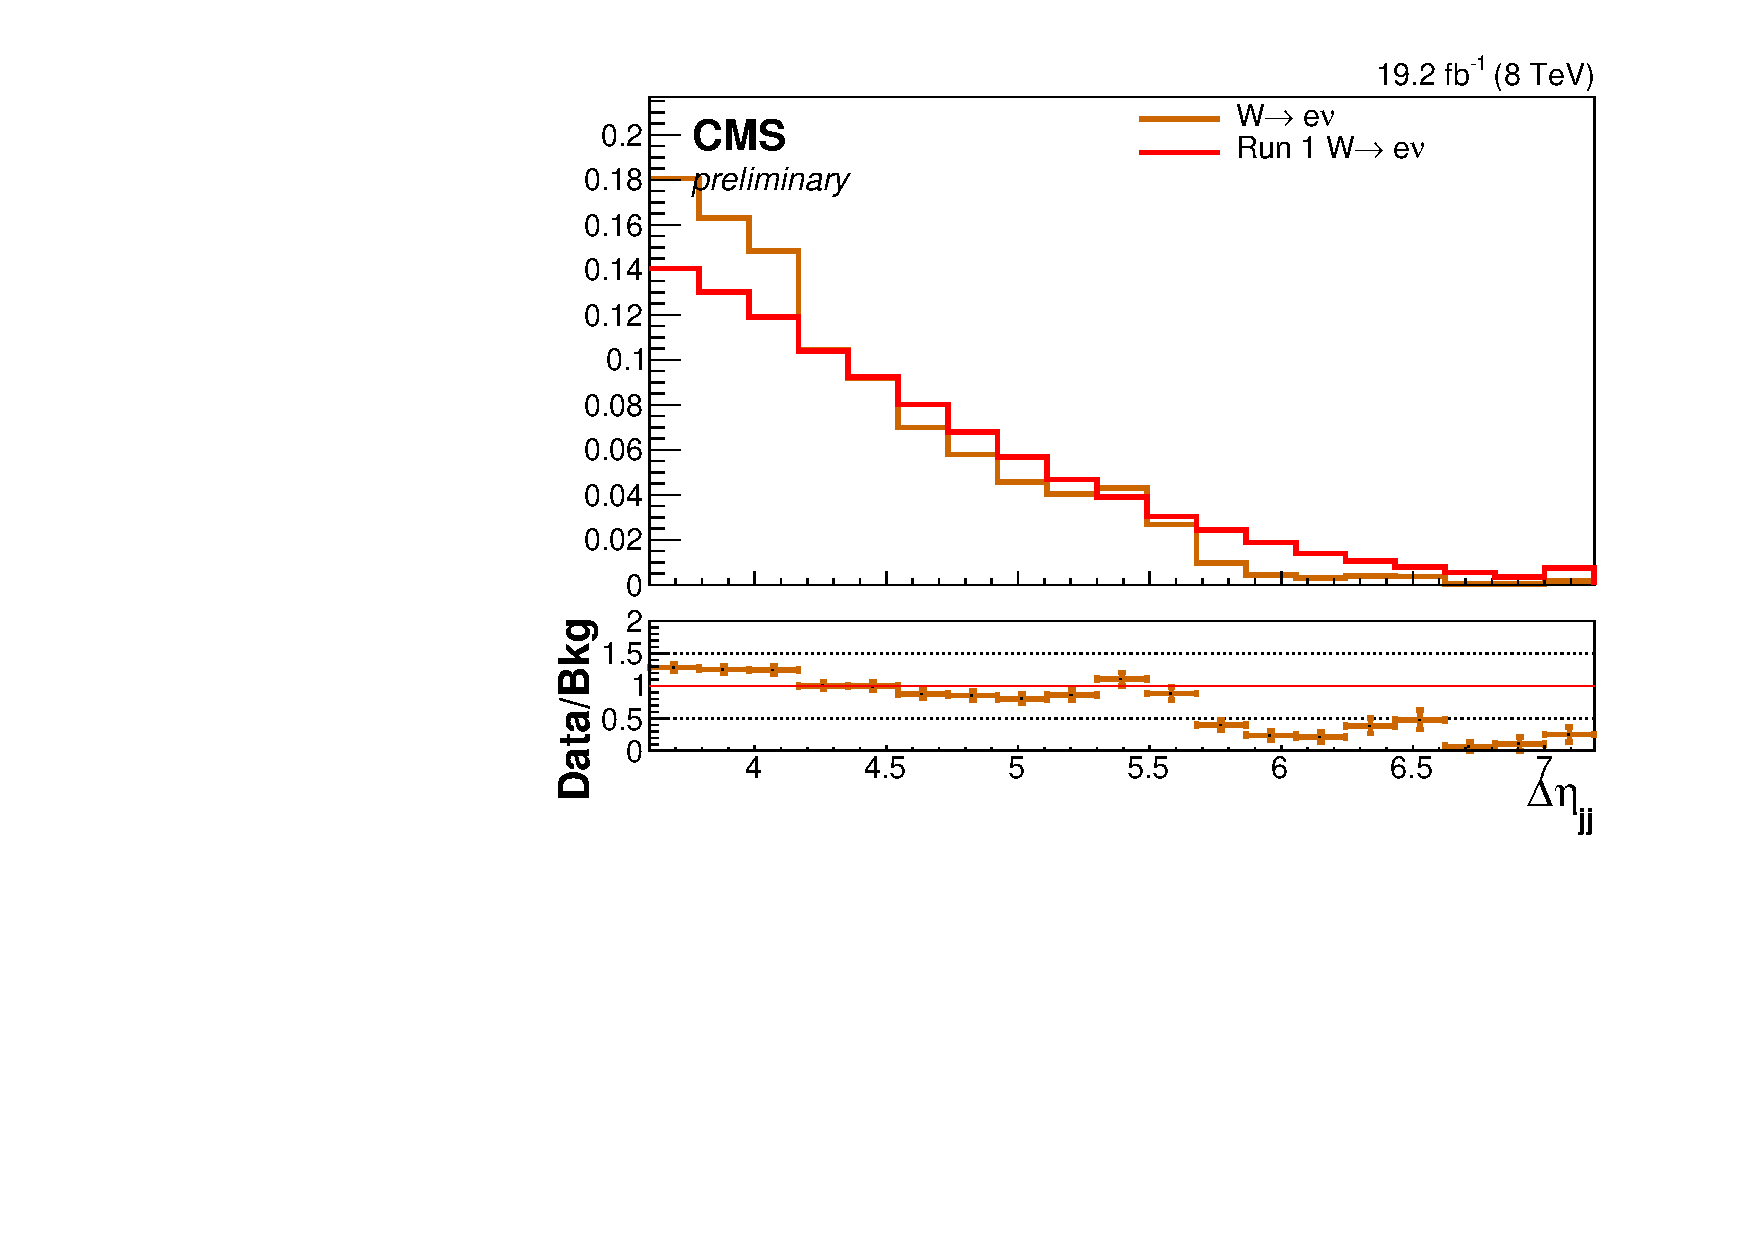
\includegraphics[width=.5\textwidth]{TalkPics/wcontplots090615/output_run1compdynoweight/enu_norm_dijet_deta.pdf}
  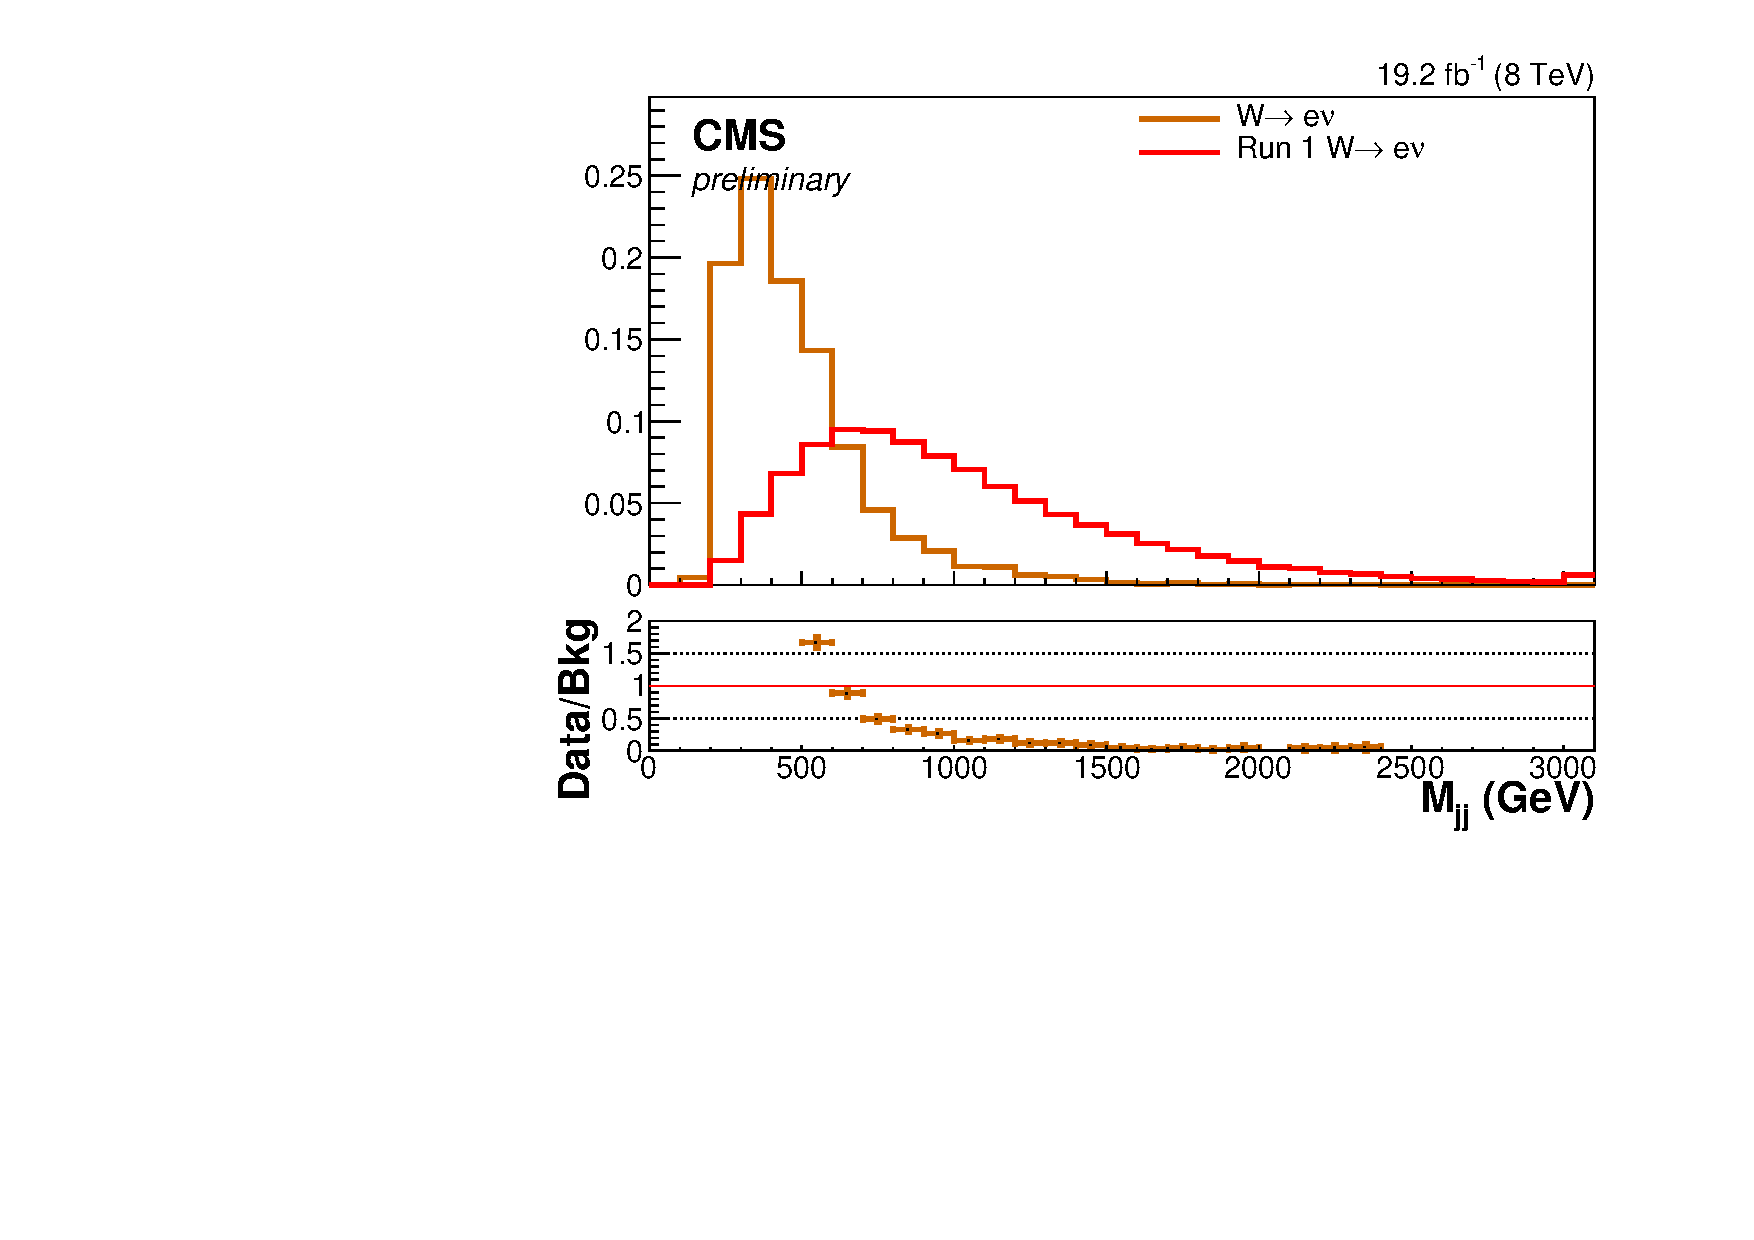
\includegraphics[width=.5\textwidth]{TalkPics/wcontplots090615/output_run1compdynoweight/enu_norm_dijet_M.pdf}
   %% \begin{block}{}
   %%   \begin{itemize}
   %%   \item 
   %%   \end{itemize}
   %% \end{block}
\end{frame}

\begin{frame}
  \frametitle{W enu Comparison: run 1 vs run 2: N jets}
  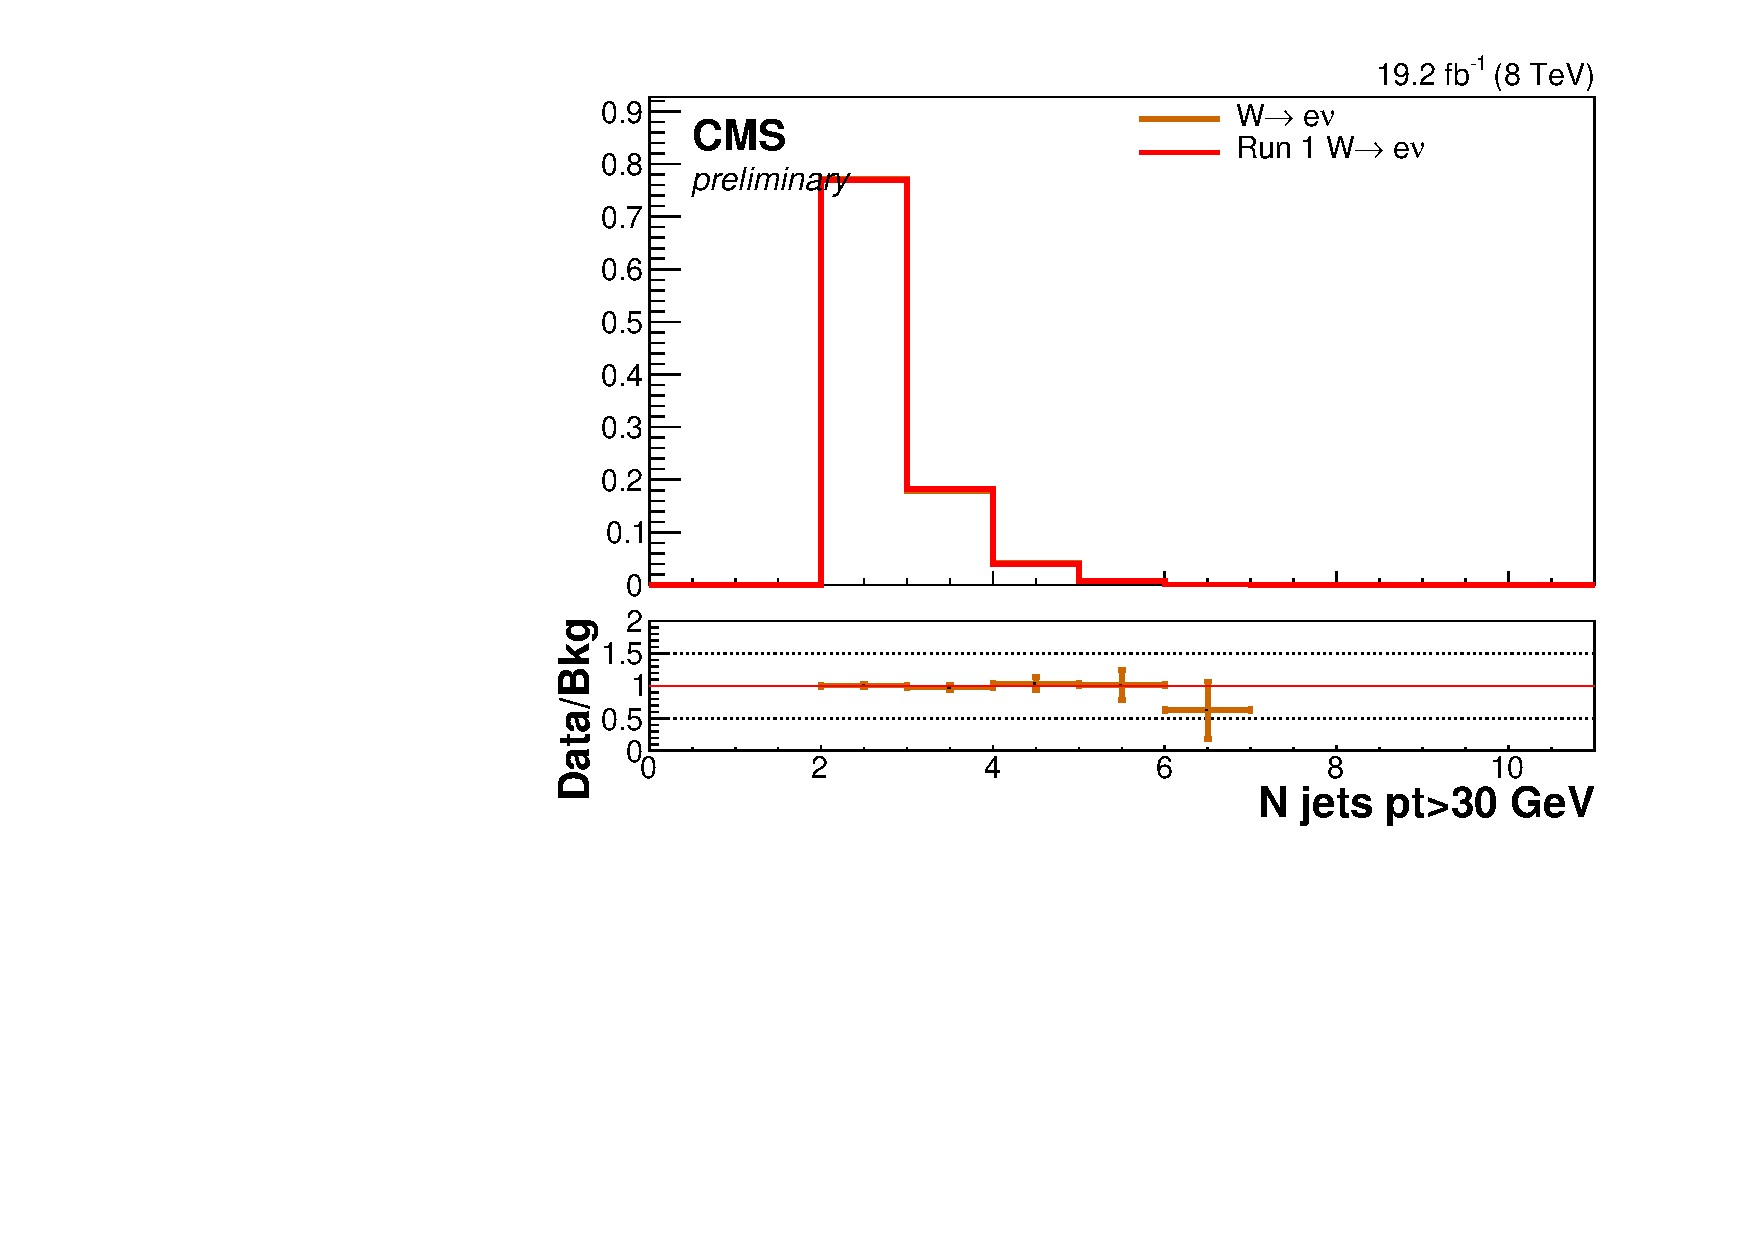
\includegraphics[width=.5\textwidth]{TalkPics/wcontplots090615/output_run1compdynoweight/enu_norm_n_jets_30.pdf}
  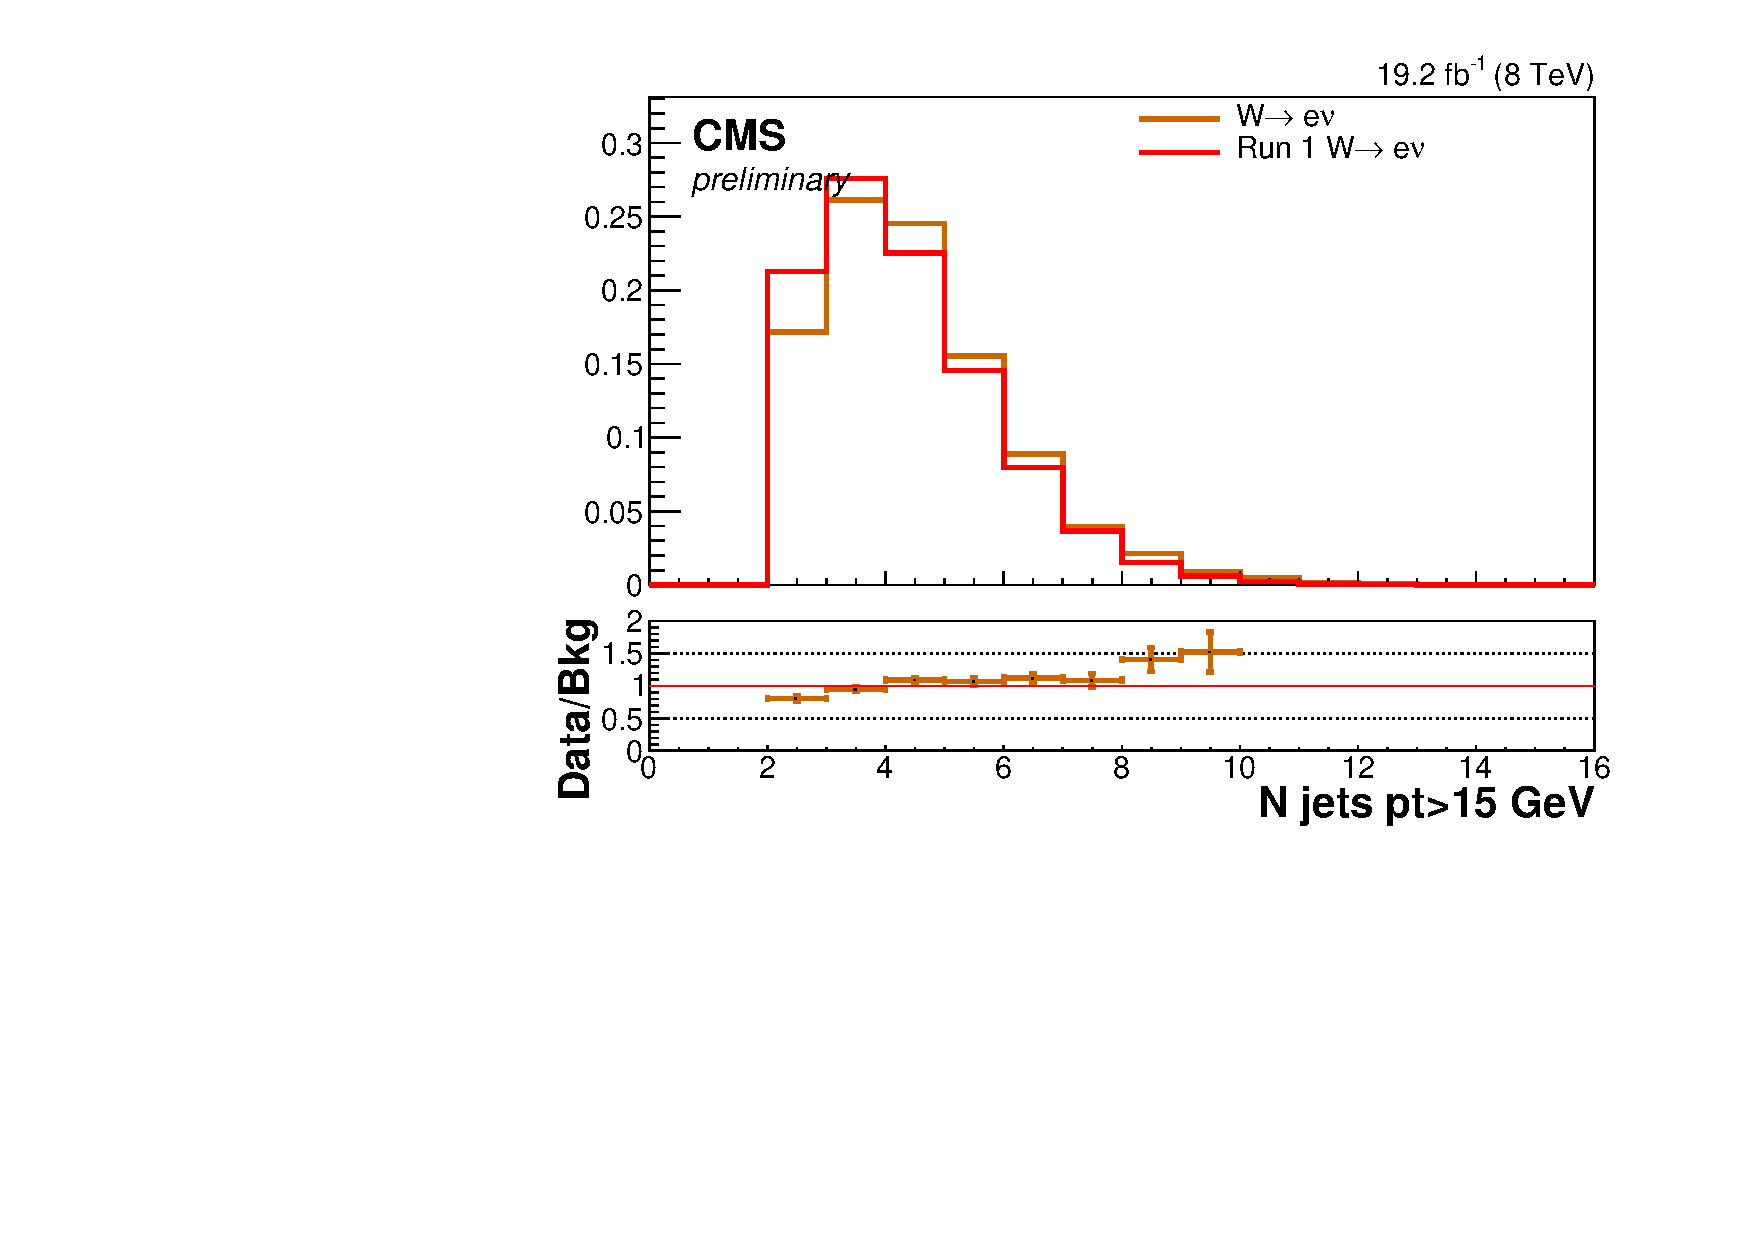
\includegraphics[width=.5\textwidth]{TalkPics/wcontplots090615/output_run1compdynoweight/enu_norm_n_jets_15.pdf}
\end{frame}

\begin{frame}
  \frametitle{W munu Comparison: run 1 vs run 2: Jet $p_{T}$}
  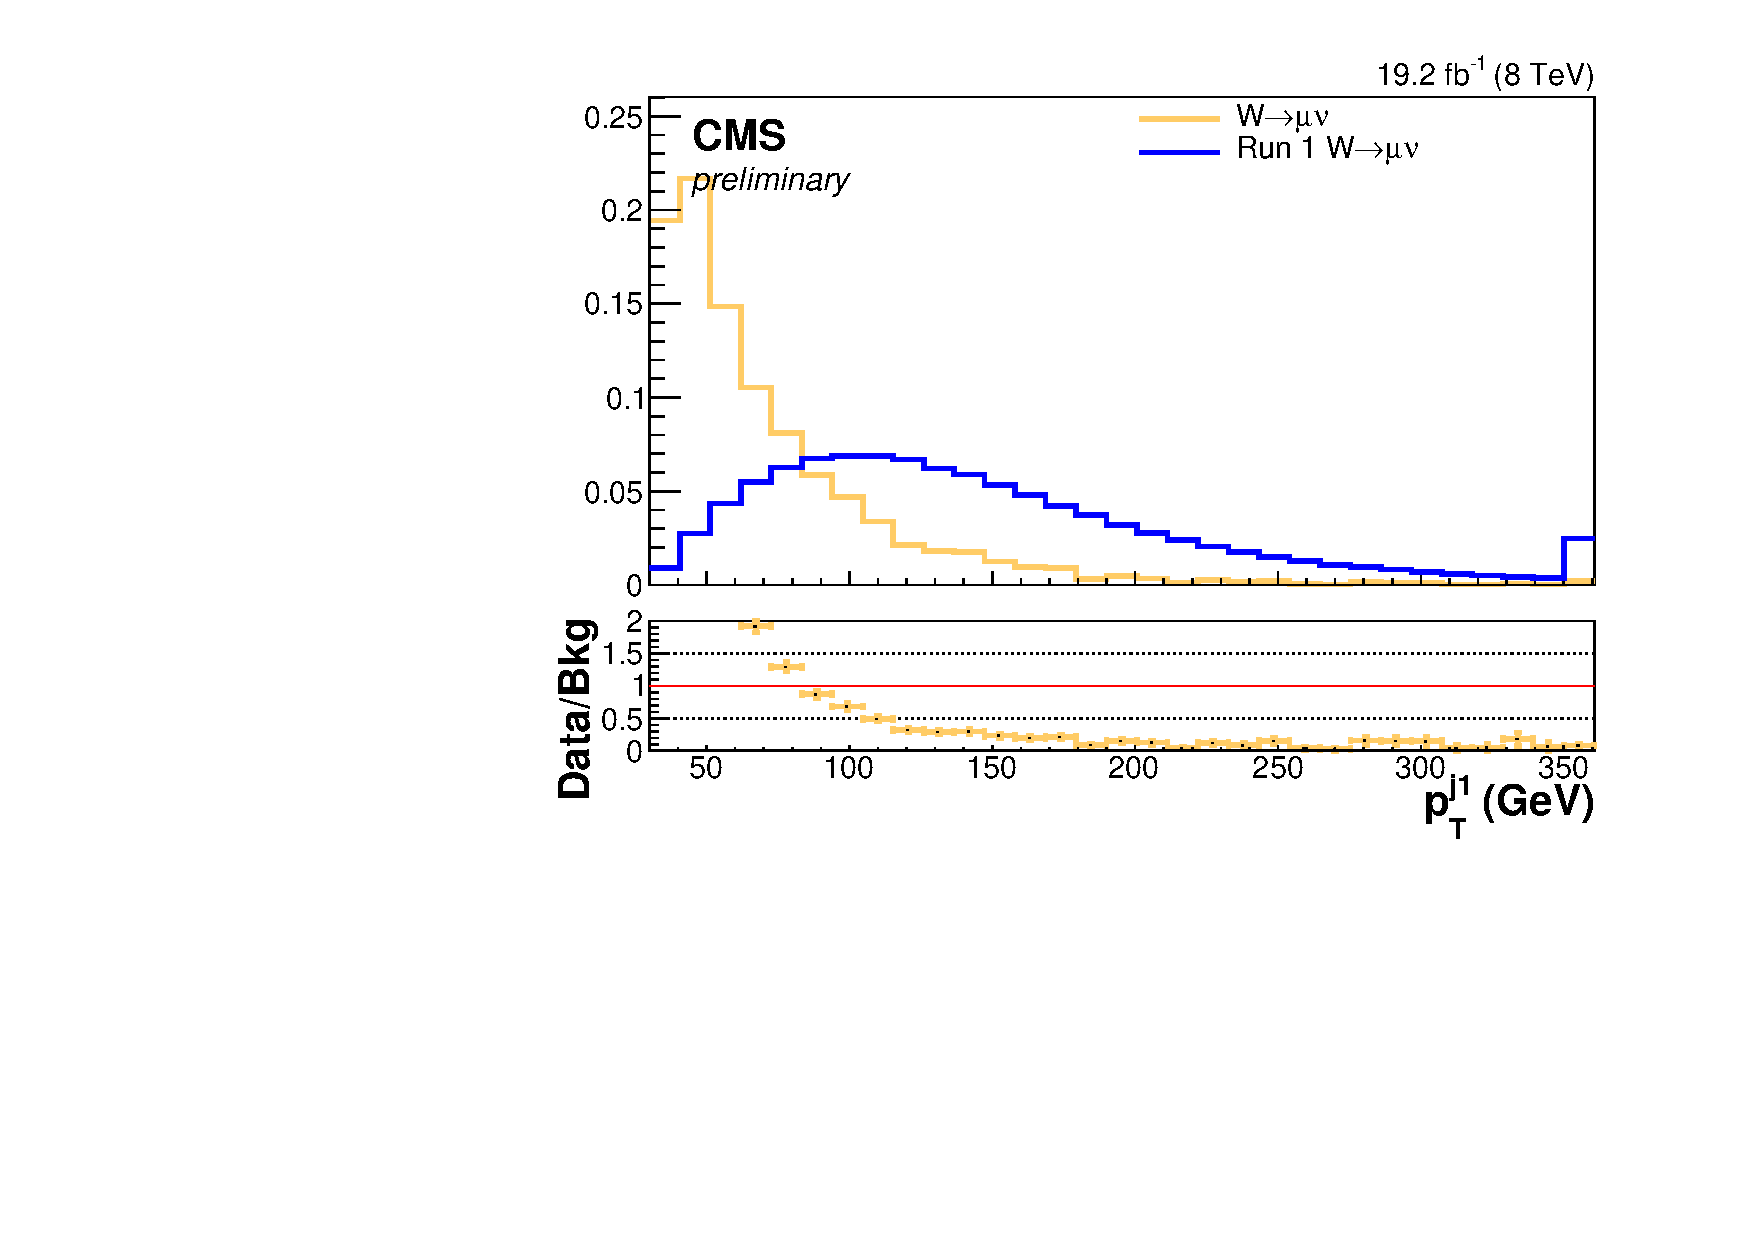
\includegraphics[width=.5\textwidth]{TalkPics/wcontplots090615/output_run1compdynoweight/munu_norm_jet1_pt.pdf}
  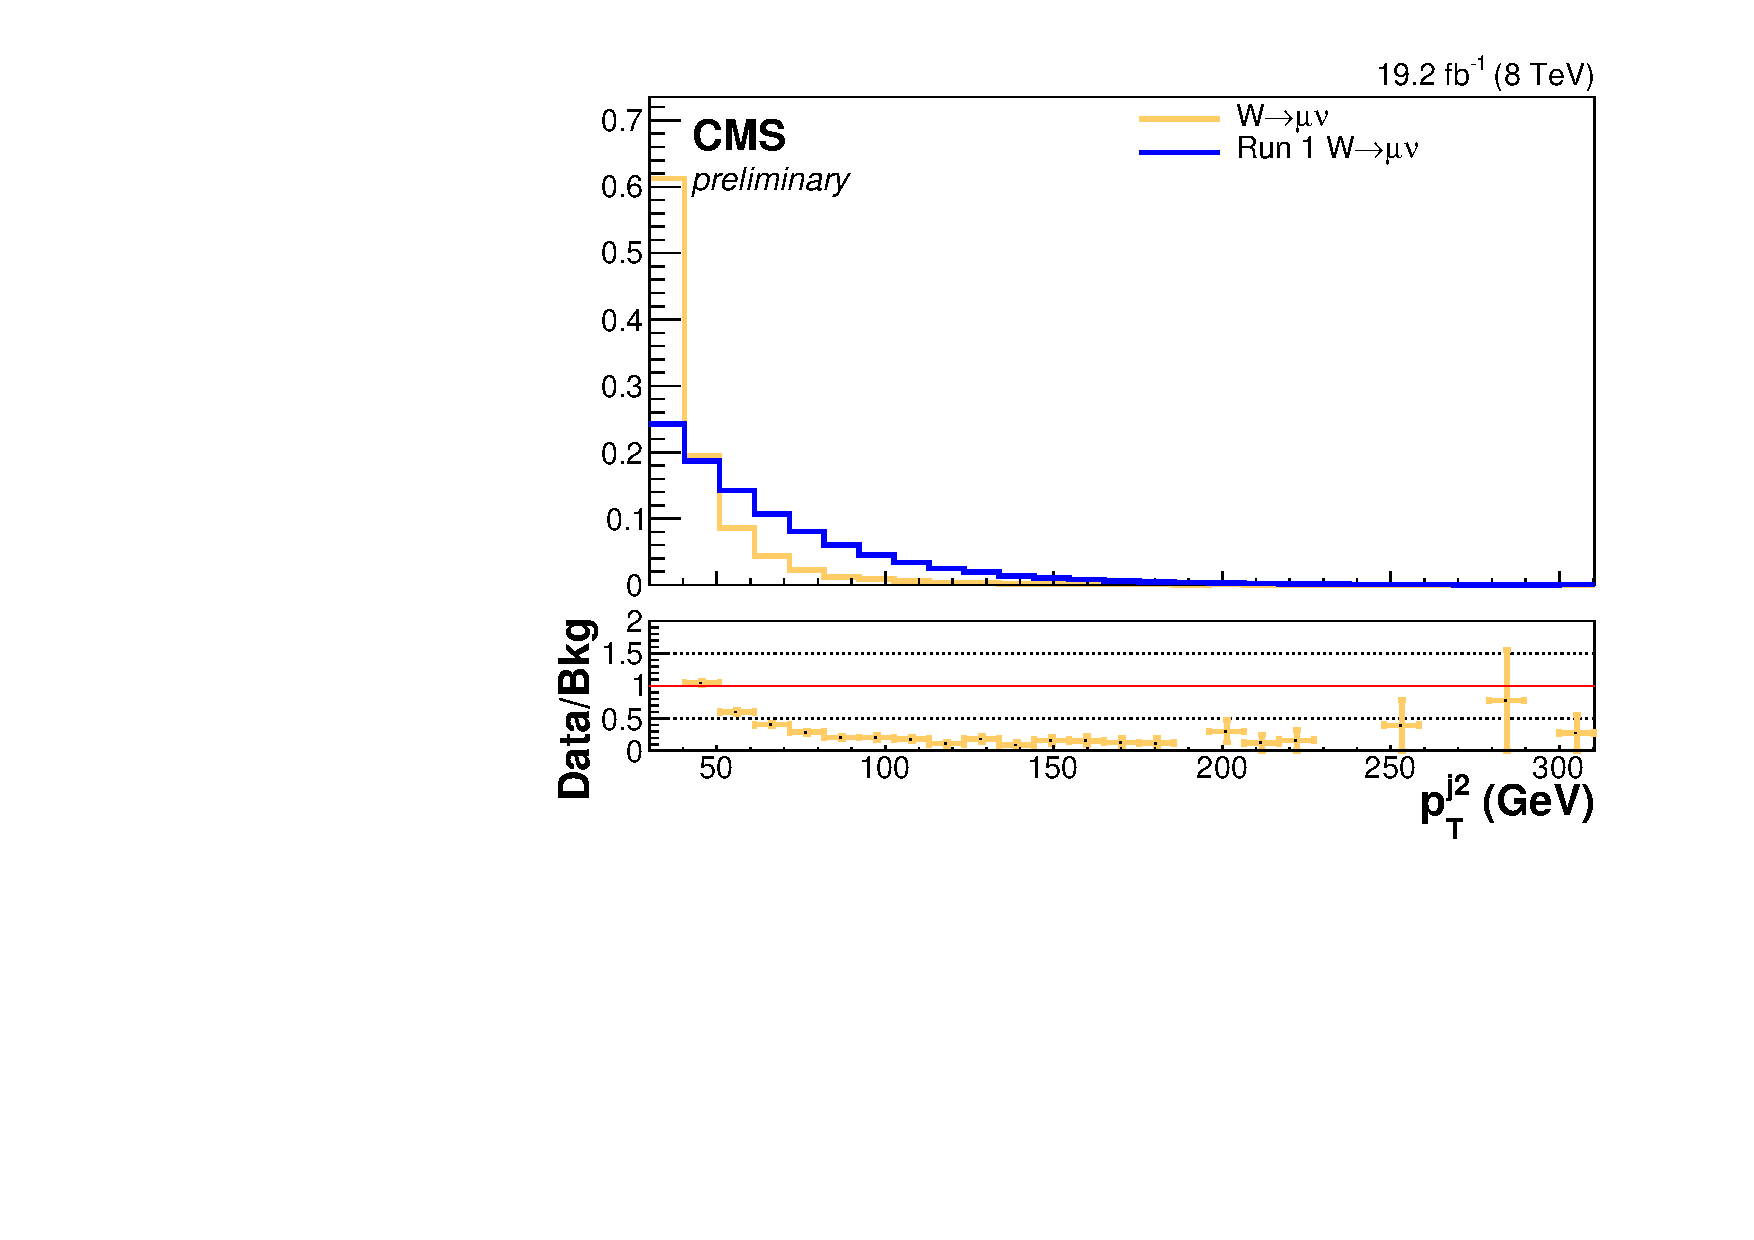
\includegraphics[width=.5\textwidth]{TalkPics/wcontplots090615/output_run1compdynoweight/munu_norm_jet2_pt.pdf}
  \begin{block}{}
    \begin{itemize}
    \item[-] Run 2 much lower could be due to met significance cut bias
    \end{itemize}
  \end{block}
\end{frame}

\begin{frame}
  \frametitle{W munu Comparison: run 1 vs run 2: Jet $\eta$}
  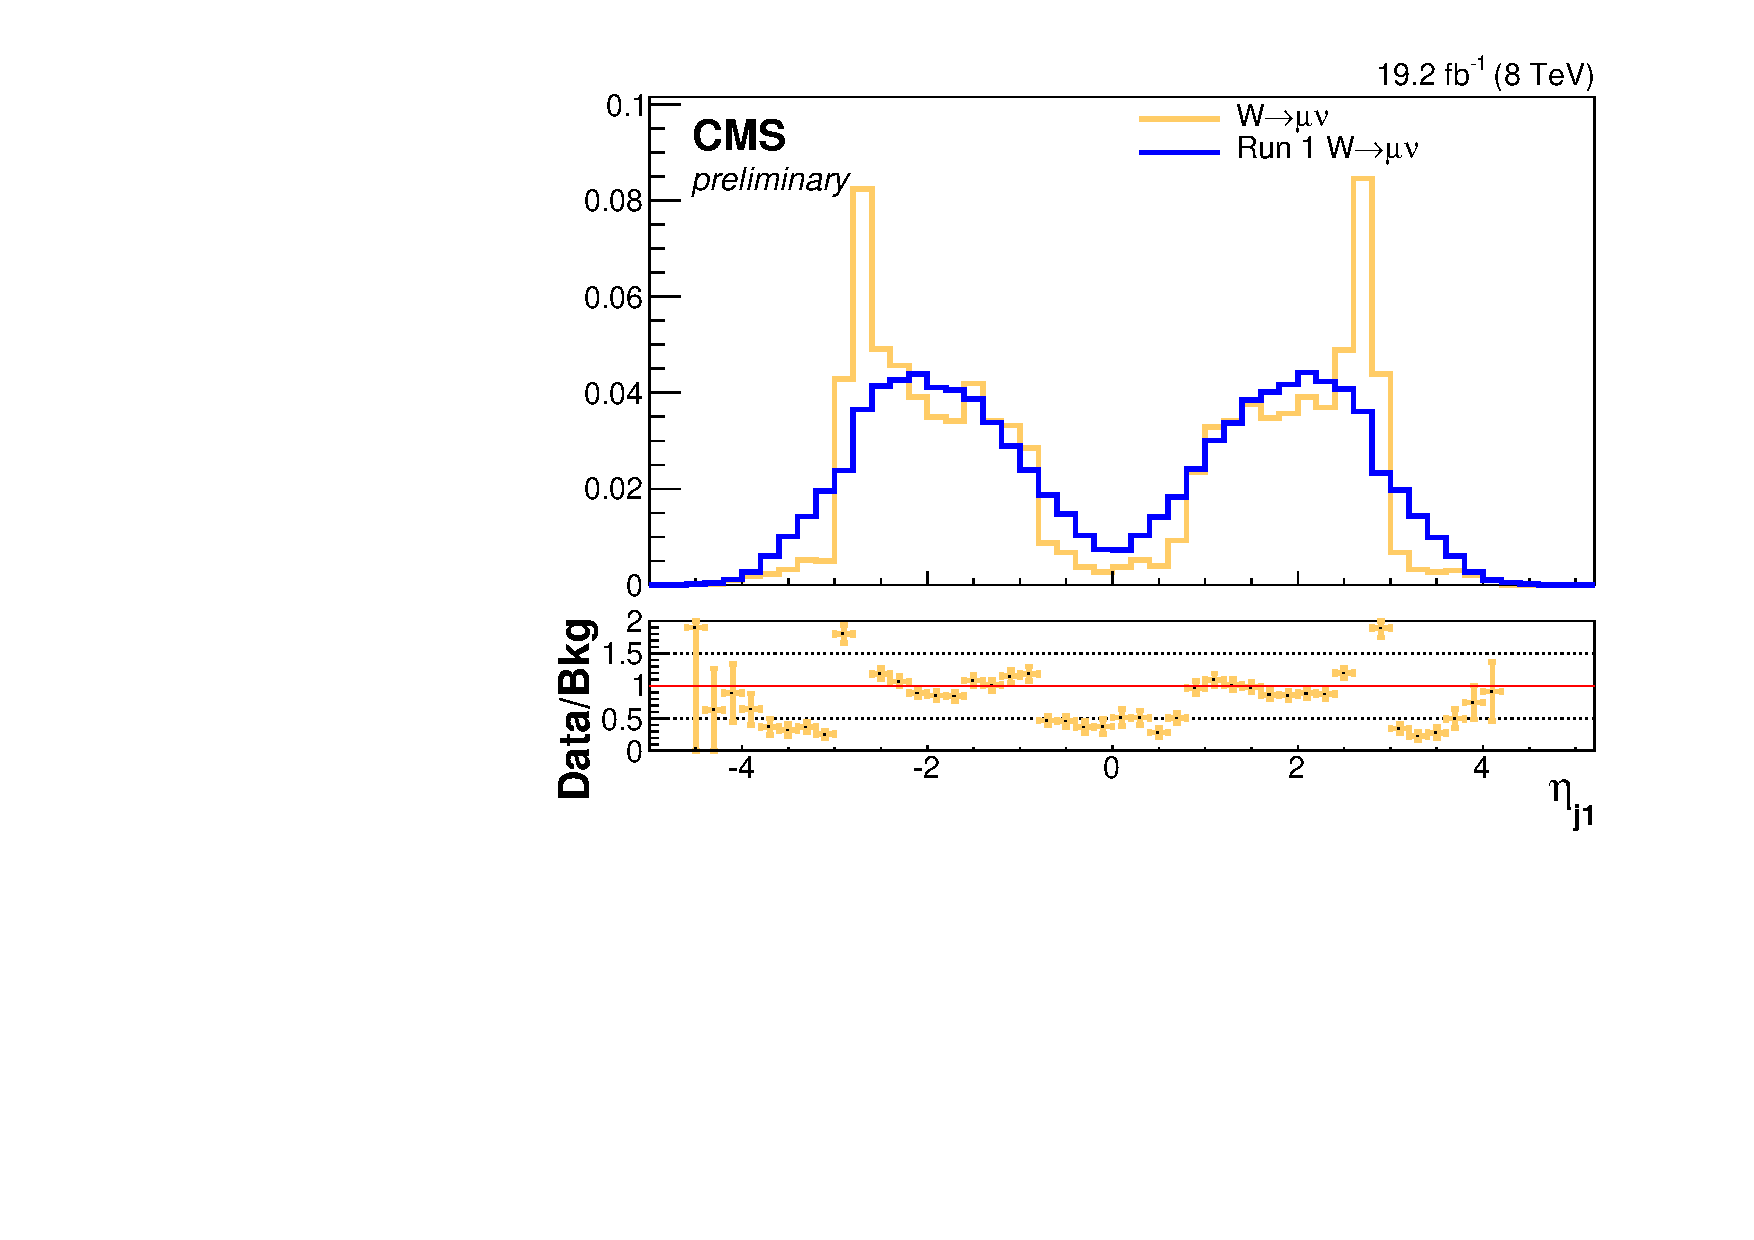
\includegraphics[width=.5\textwidth]{TalkPics/wcontplots090615/output_run1compdynoweight/munu_norm_jet1_eta.pdf}
  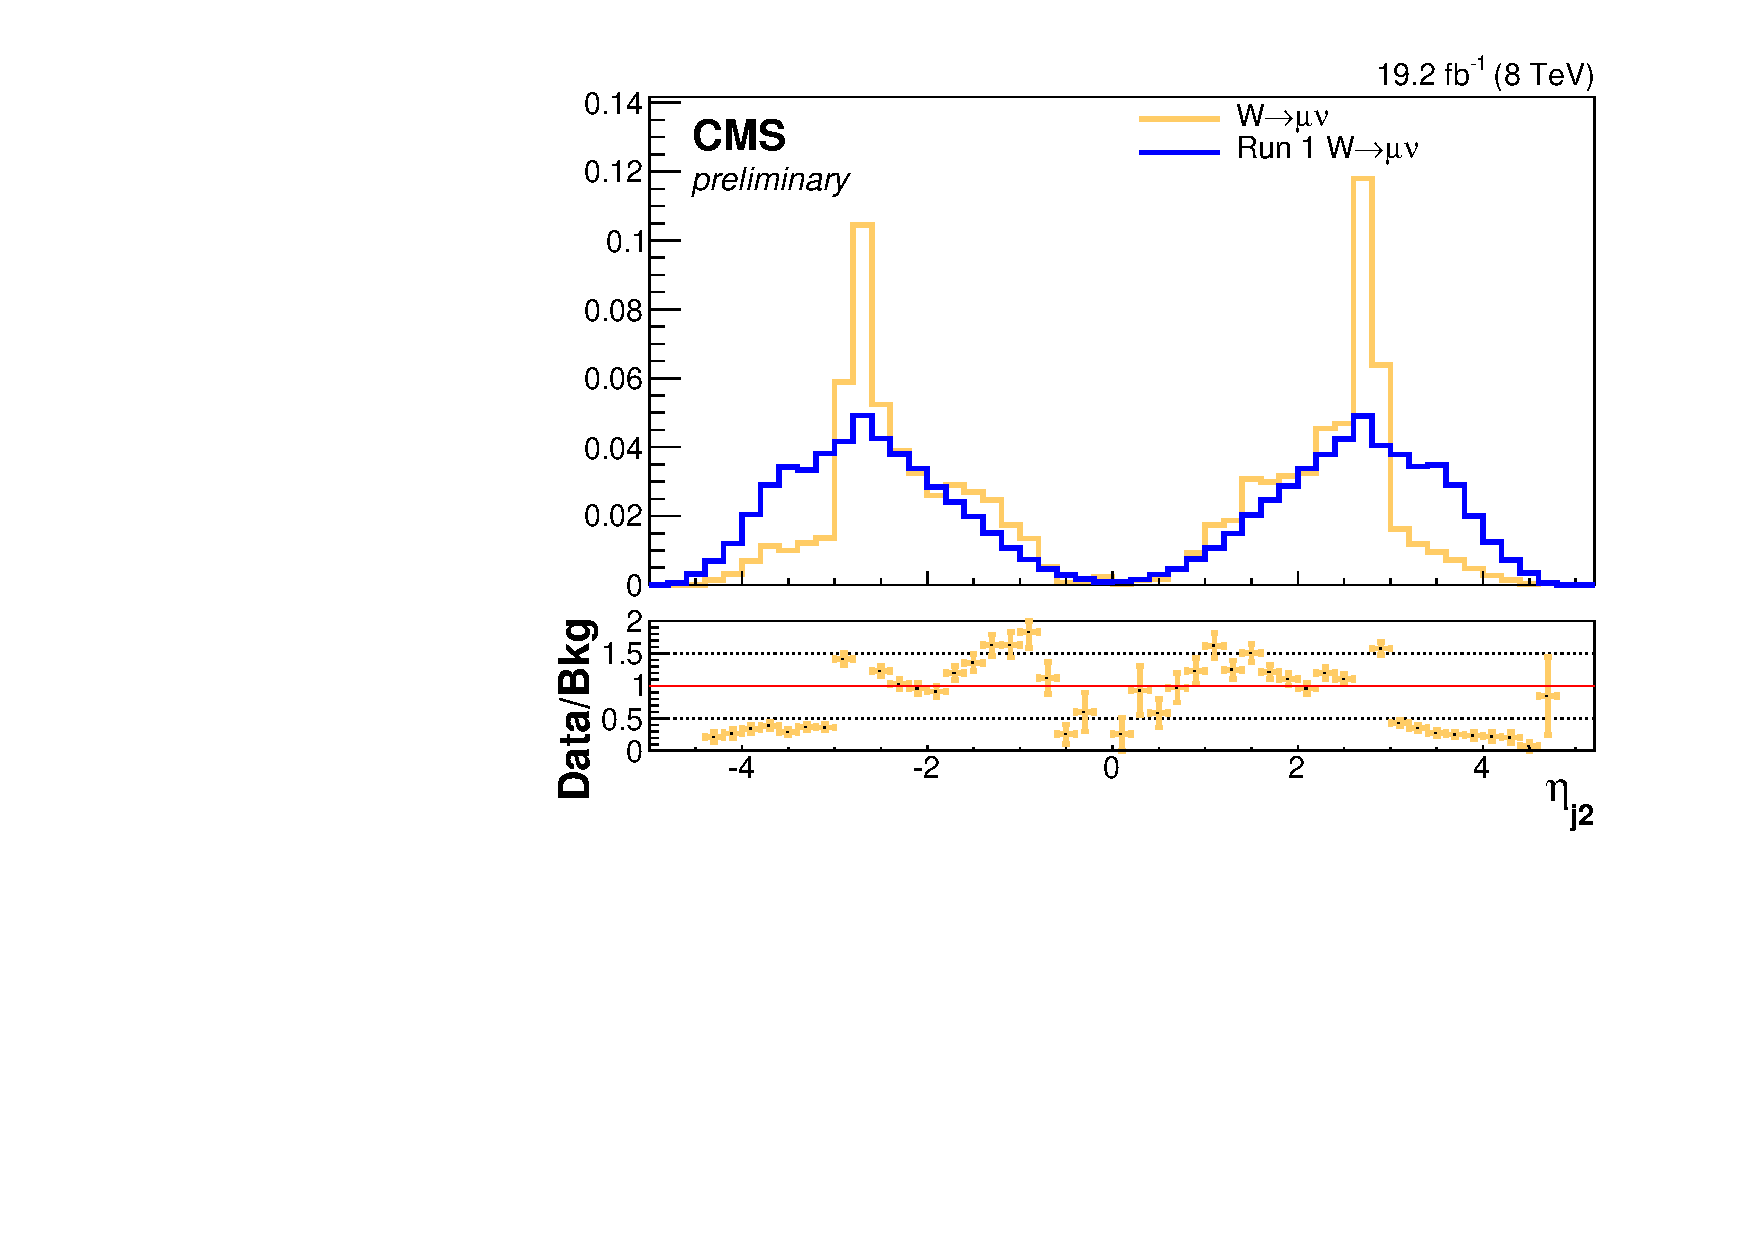
\includegraphics[width=.5\textwidth]{TalkPics/wcontplots090615/output_run1compdynoweight/munu_norm_jet2_eta.pdf}
  \begin{block}{}
    \begin{itemize}
    \item Ears still apparent
    \end{itemize}
  \end{block}
\end{frame}

\begin{frame}
  \frametitle{W munu Comparison: run 1 vs run 2: Jet $\phi$}
  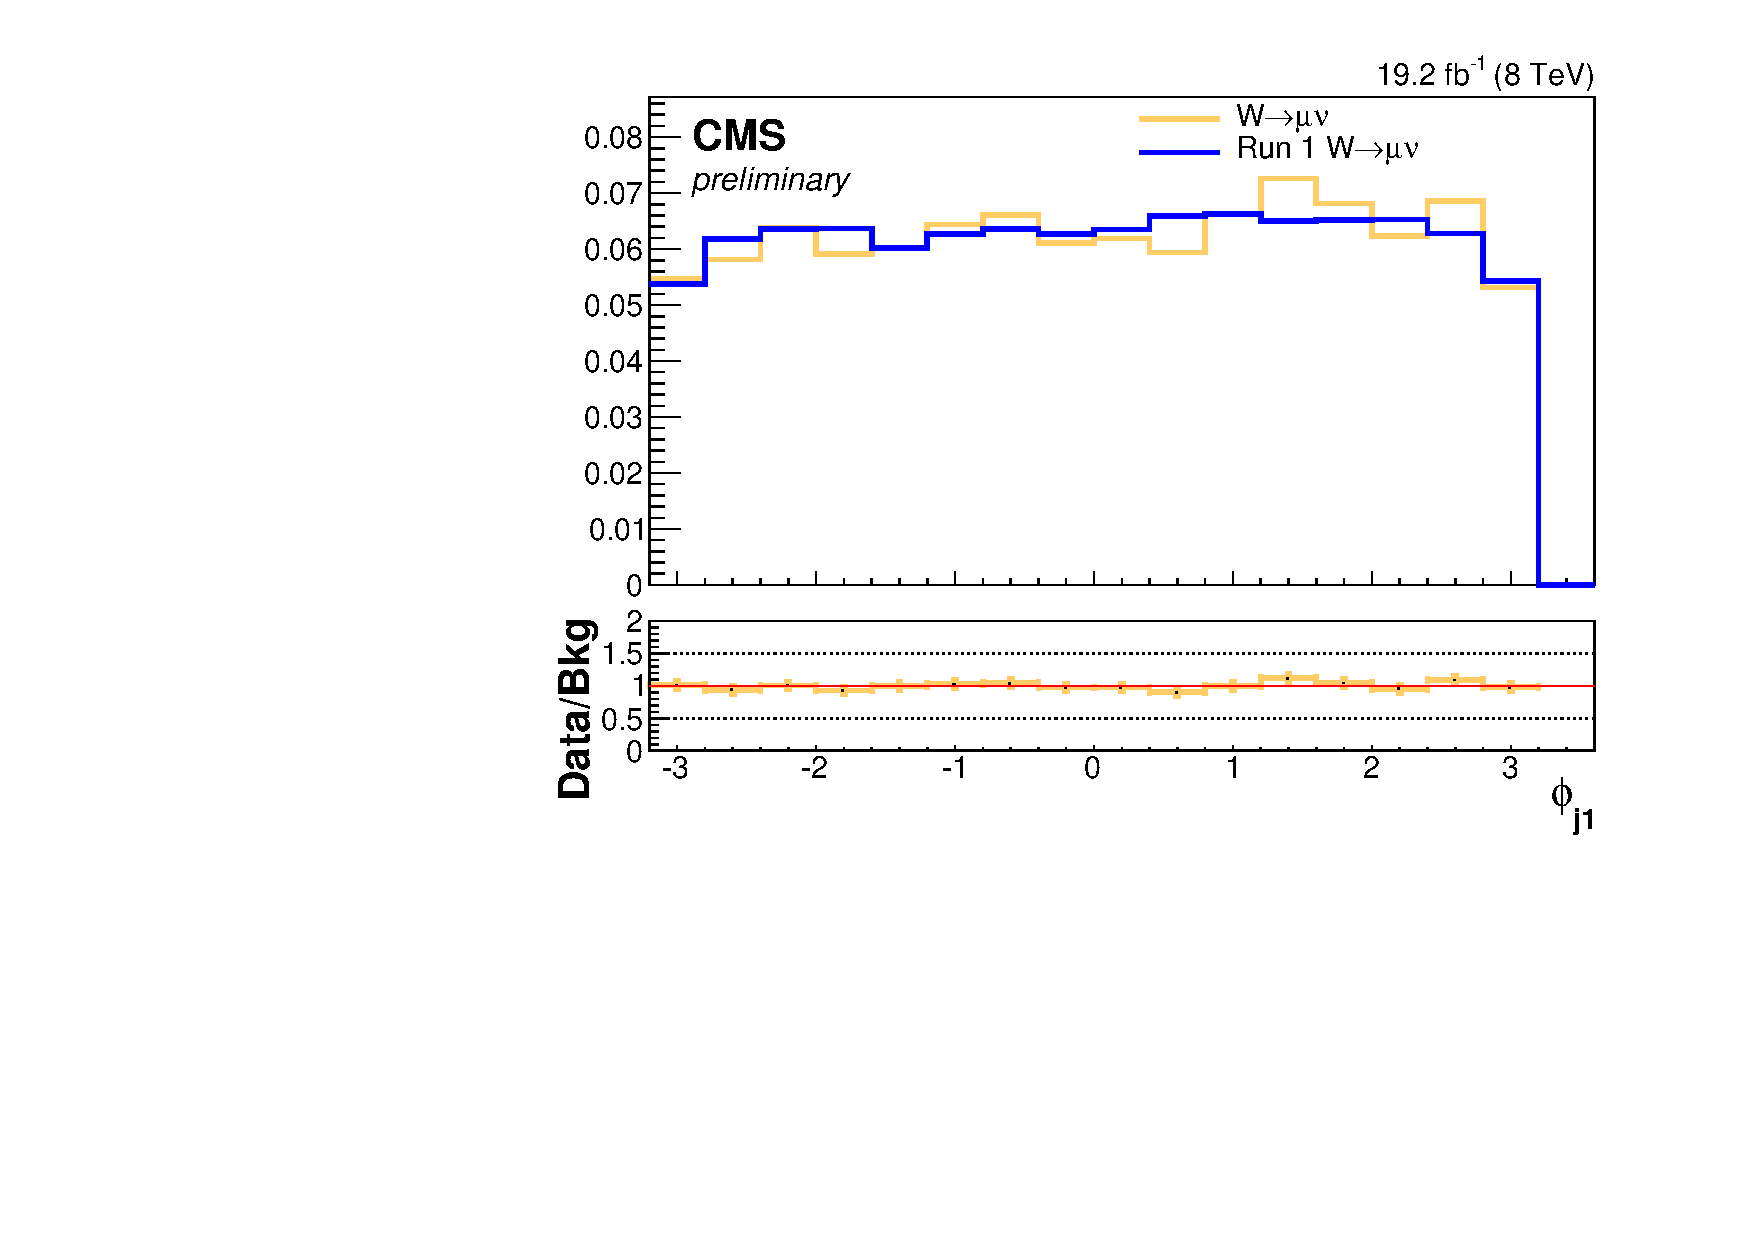
\includegraphics[width=.5\textwidth]{TalkPics/wcontplots090615/output_run1compdynoweight/munu_norm_jet1_phi.pdf}
  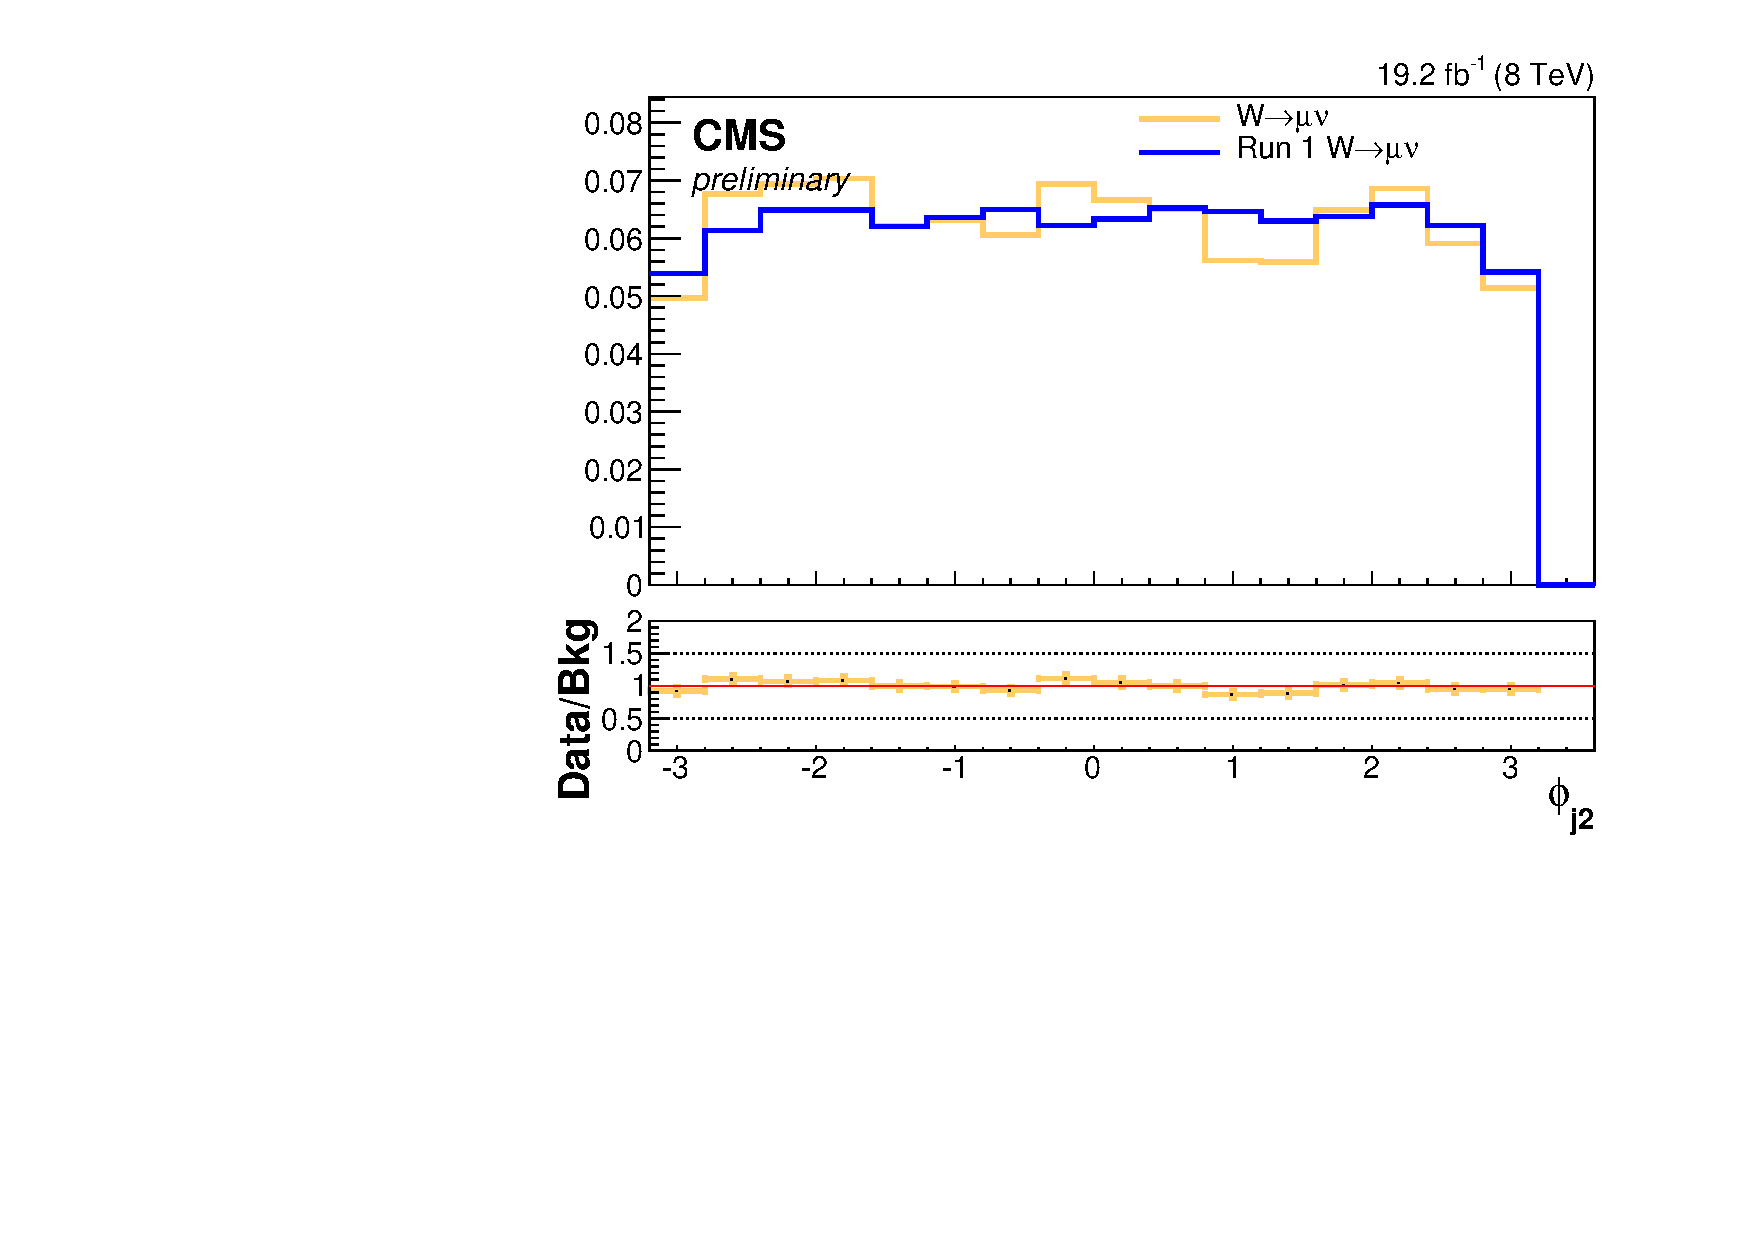
\includegraphics[width=.5\textwidth]{TalkPics/wcontplots090615/output_run1compdynoweight/munu_norm_jet2_phi.pdf}
  \begin{block}{}
    \begin{itemize}
    \item $\phi$ distributions look similar within stat error
    \end{itemize}
  \end{block}
\end{frame}

\begin{frame}
  \frametitle{W munu Comparison: run 1 vs run 2: Met}
  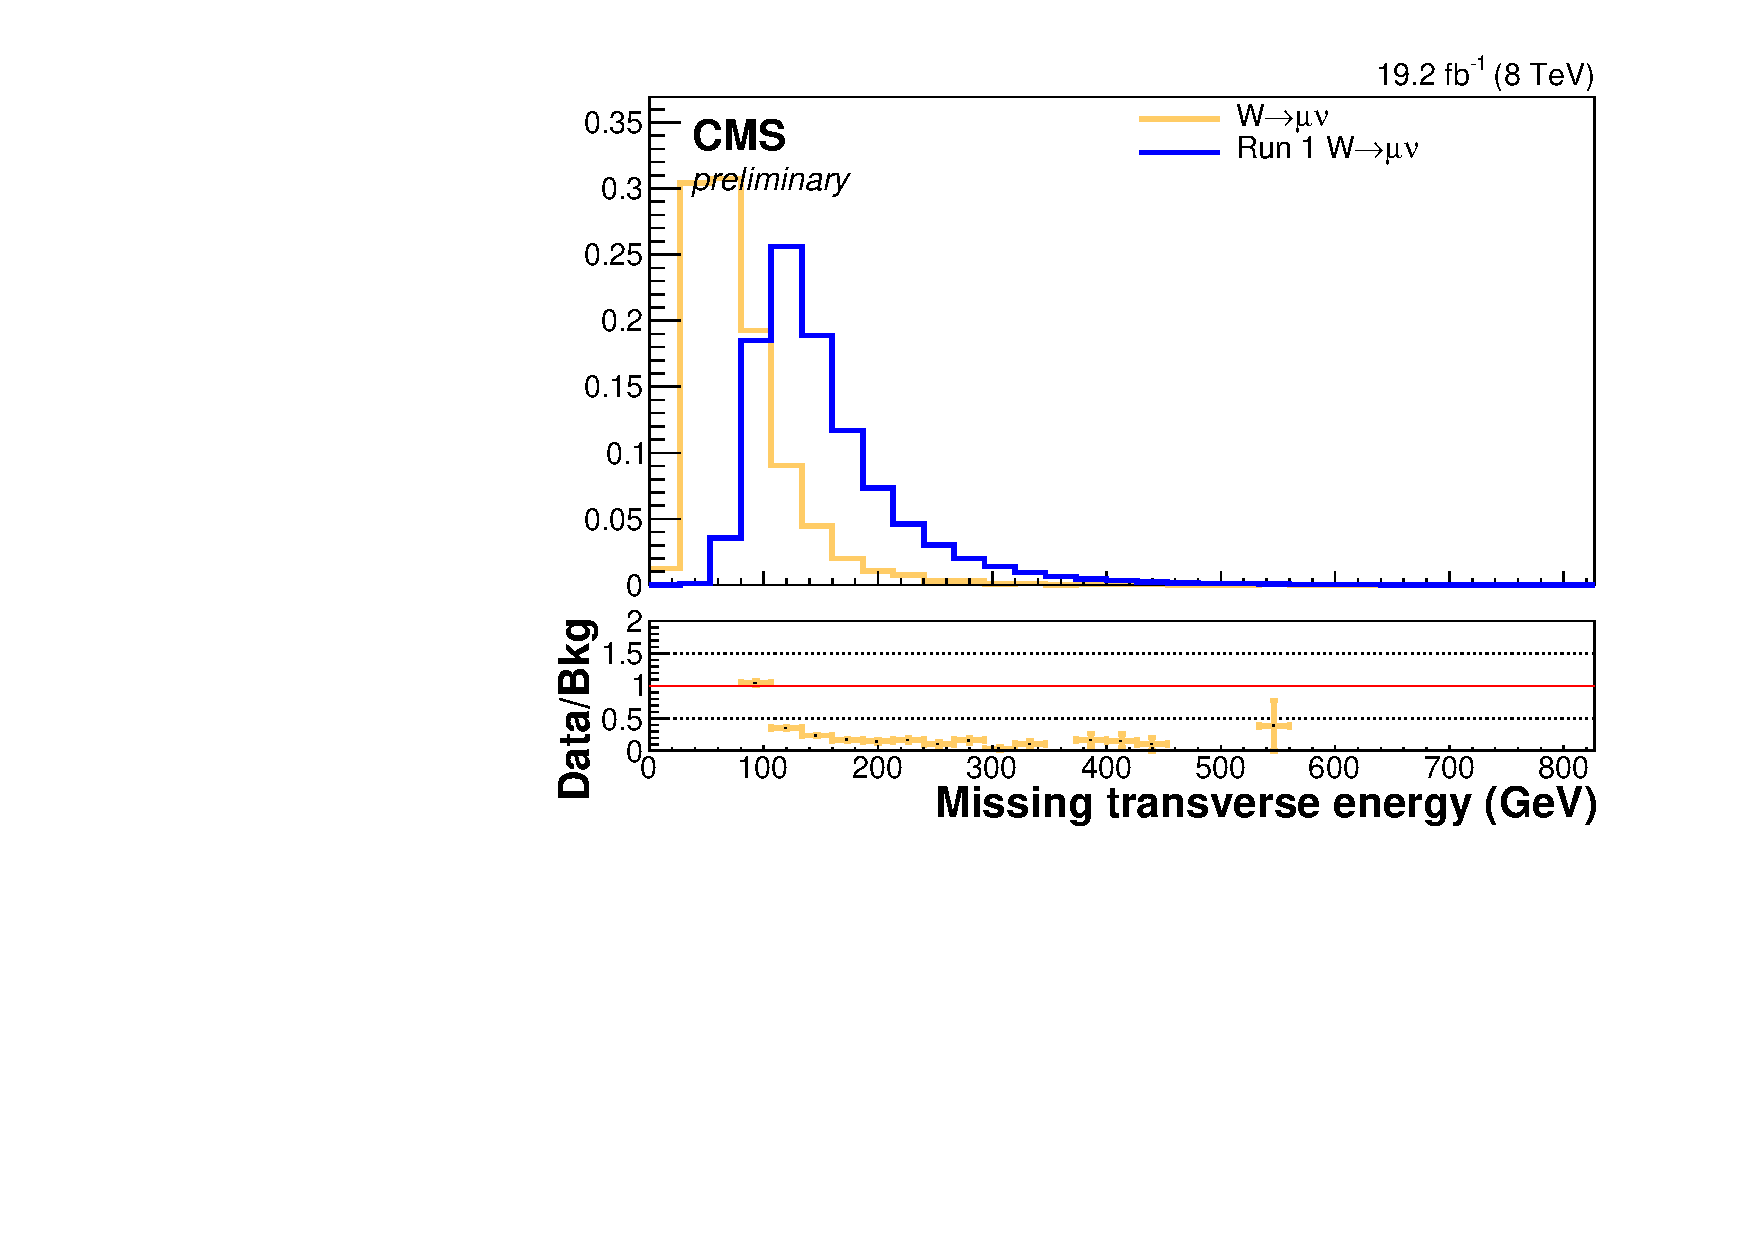
\includegraphics[width=.5\textwidth]{TalkPics/wcontplots090615/output_run1compdynoweight/munu_norm_metnomuons.pdf}
  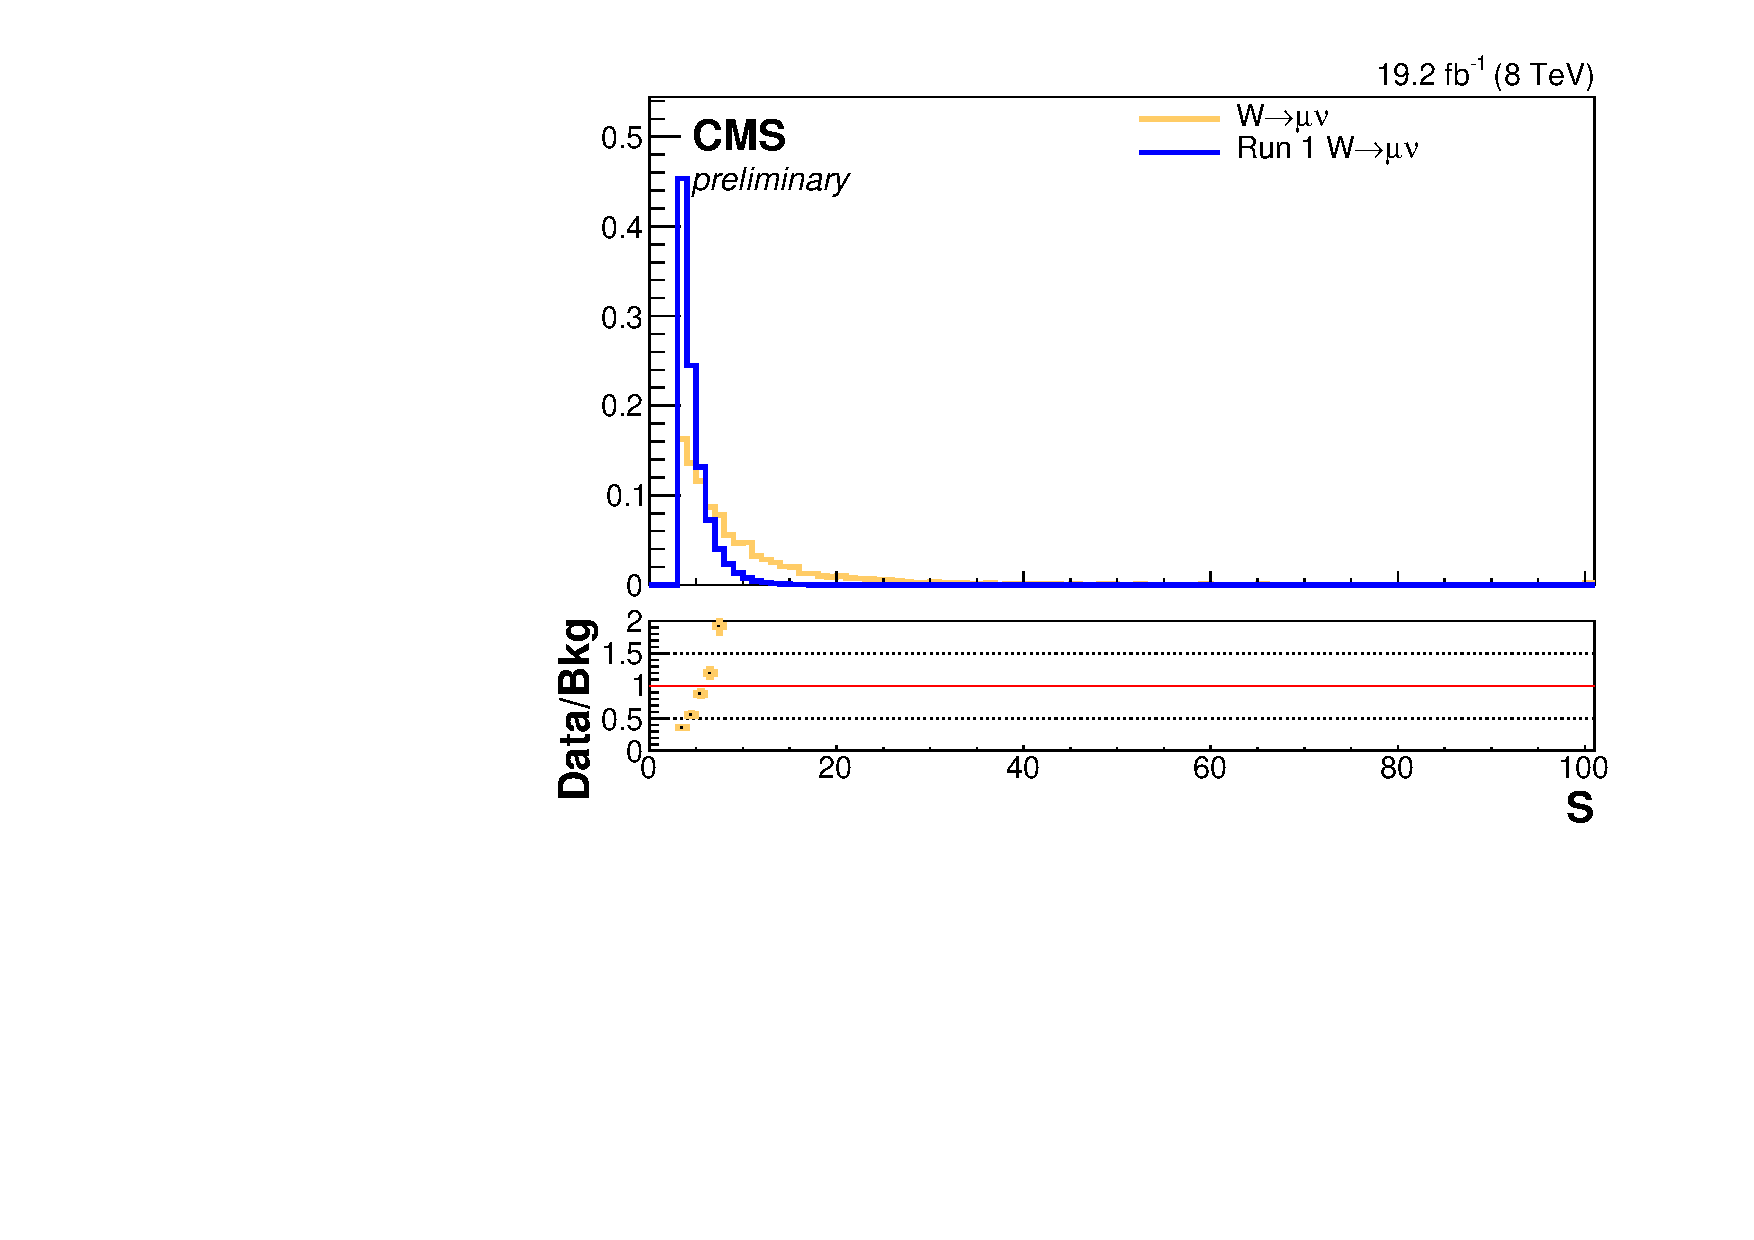
\includegraphics[width=.5\textwidth]{TalkPics/wcontplots090615/output_run1compdynoweight/munu_norm_metnomu_significance.pdf}
  \begin{block}{}
    \begin{itemize}
    \item Metnomu lower for run 2
    \item Met significance is a different variable in miniAOD to the one we used in run 1
    \end{itemize}
  \end{block}
\end{frame}

\begin{frame}
  \frametitle{W munu Comparison: run 1 vs run 2: $\Delta\phi$ variables}
  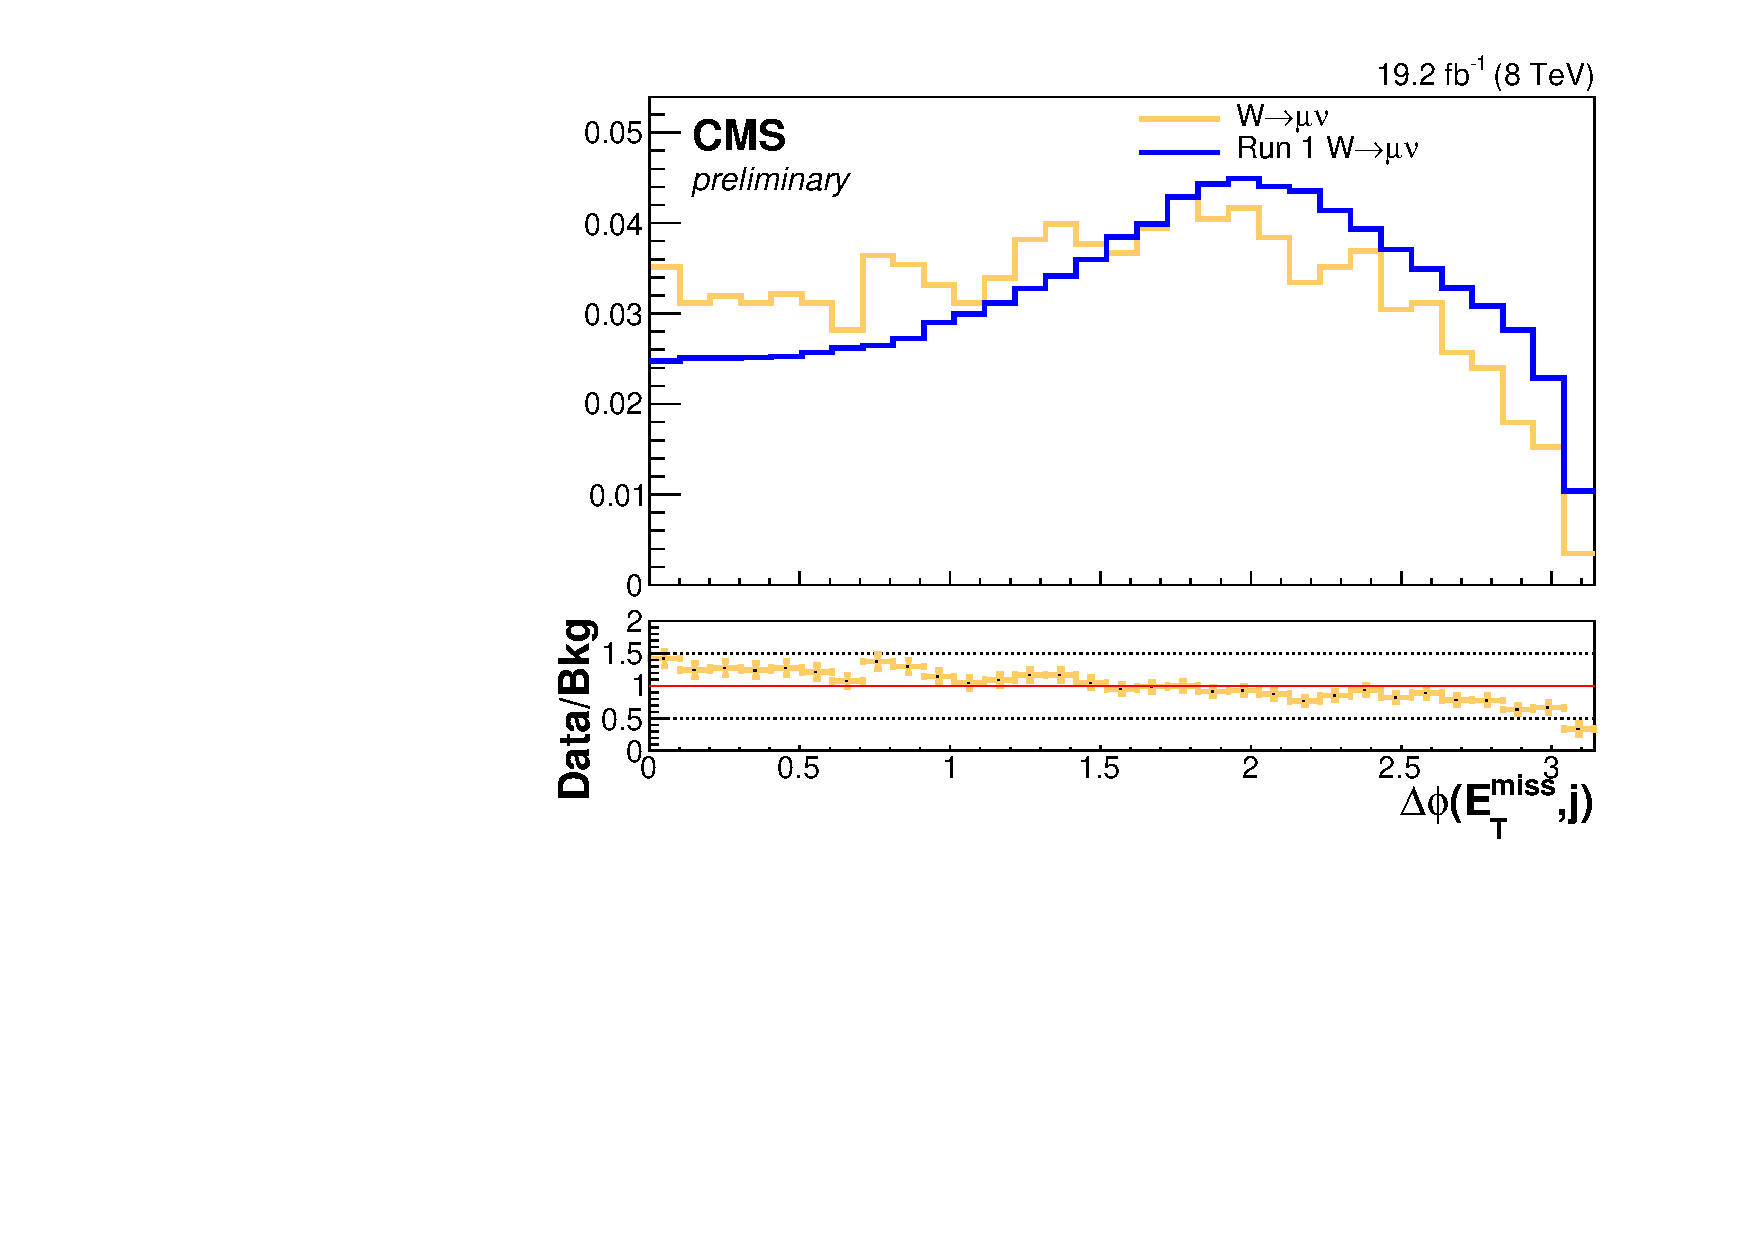
\includegraphics[width=.5\textwidth]{TalkPics/wcontplots090615/output_run1compdynoweight/munu_norm_alljetsmetnomu_mindphi.pdf}
  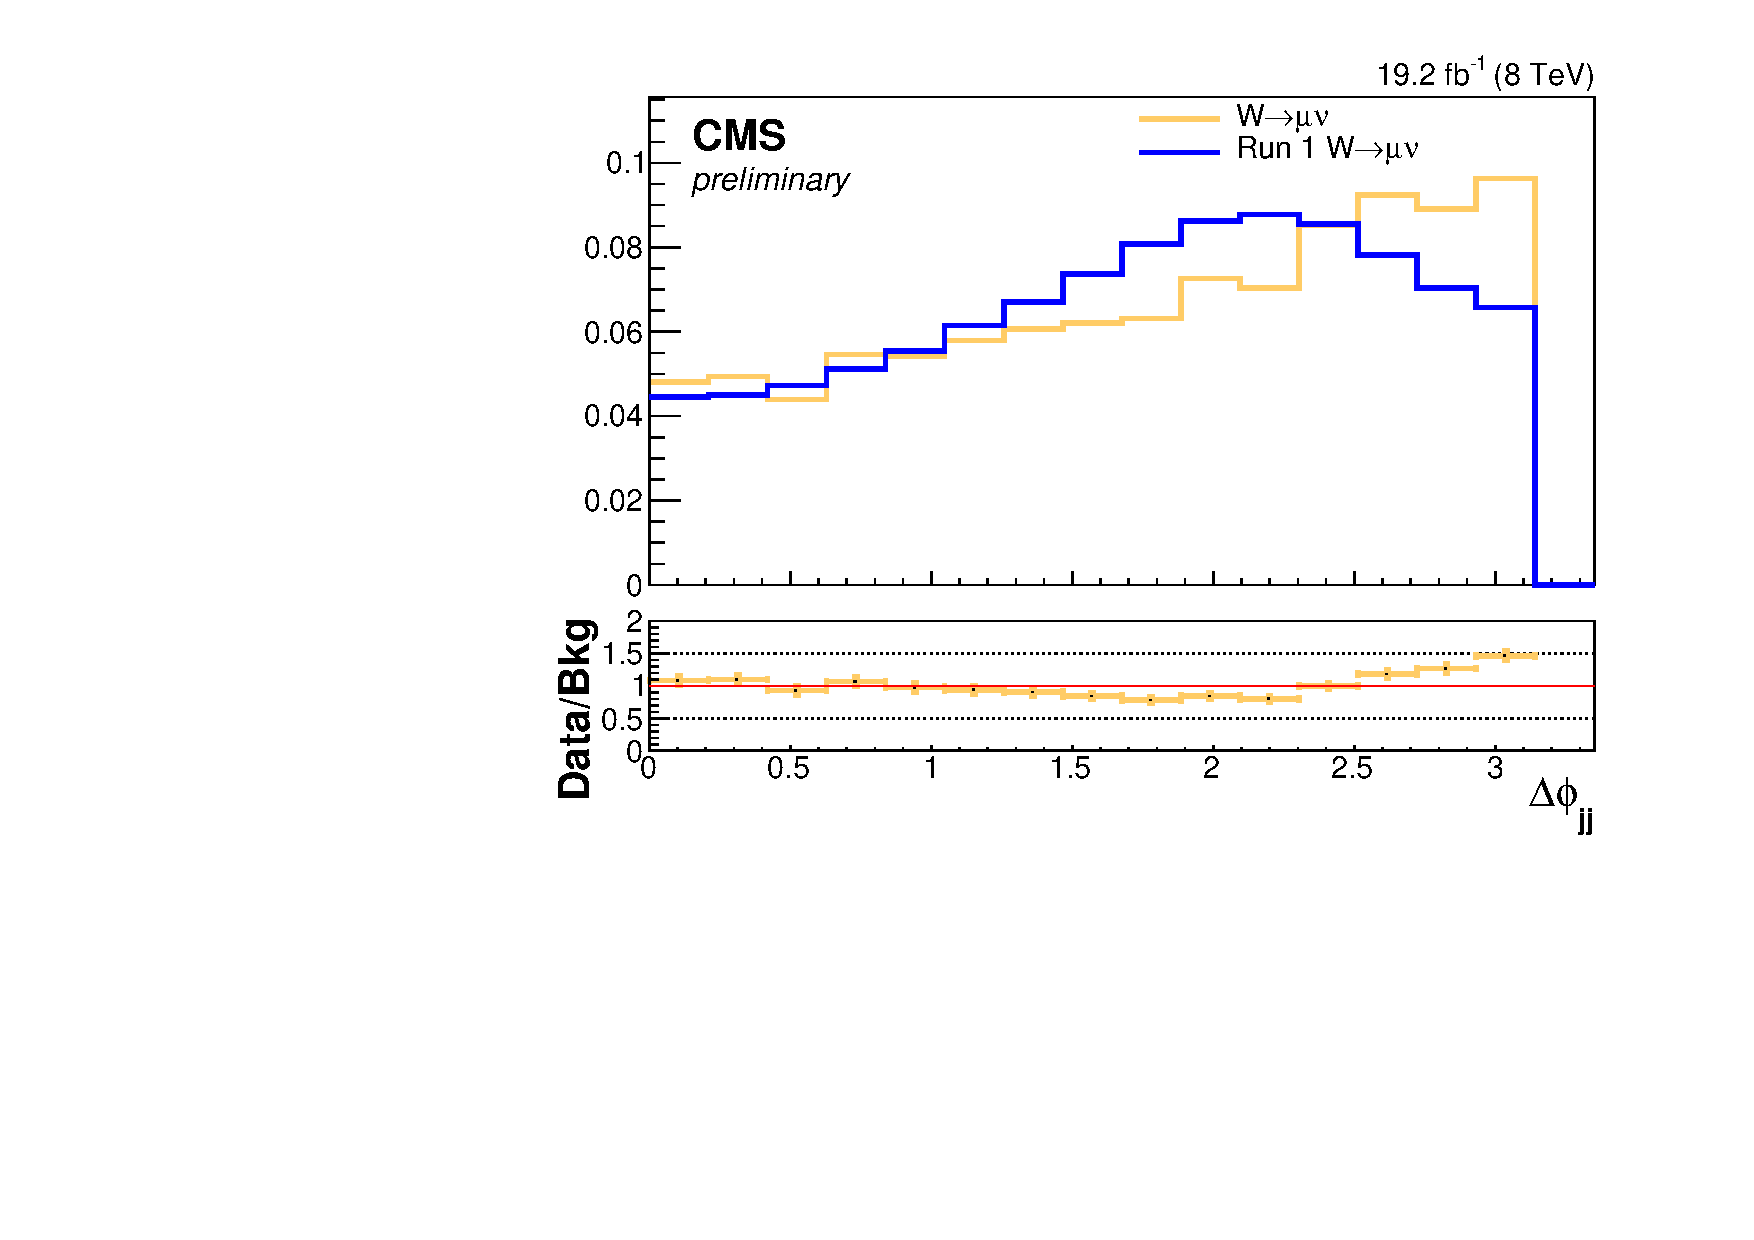
\includegraphics[width=.5\textwidth]{TalkPics/wcontplots090615/output_run1compdynoweight/munu_norm_dijet_dphi.pdf}
  \begin{block}{}
    \begin{itemize}
    \item Difference could be due to met significance bias
    \end{itemize}
  \end{block}
\end{frame}

\begin{frame}
  \frametitle{W munu Comparison: run 1 vs run 2: dijet variables}
  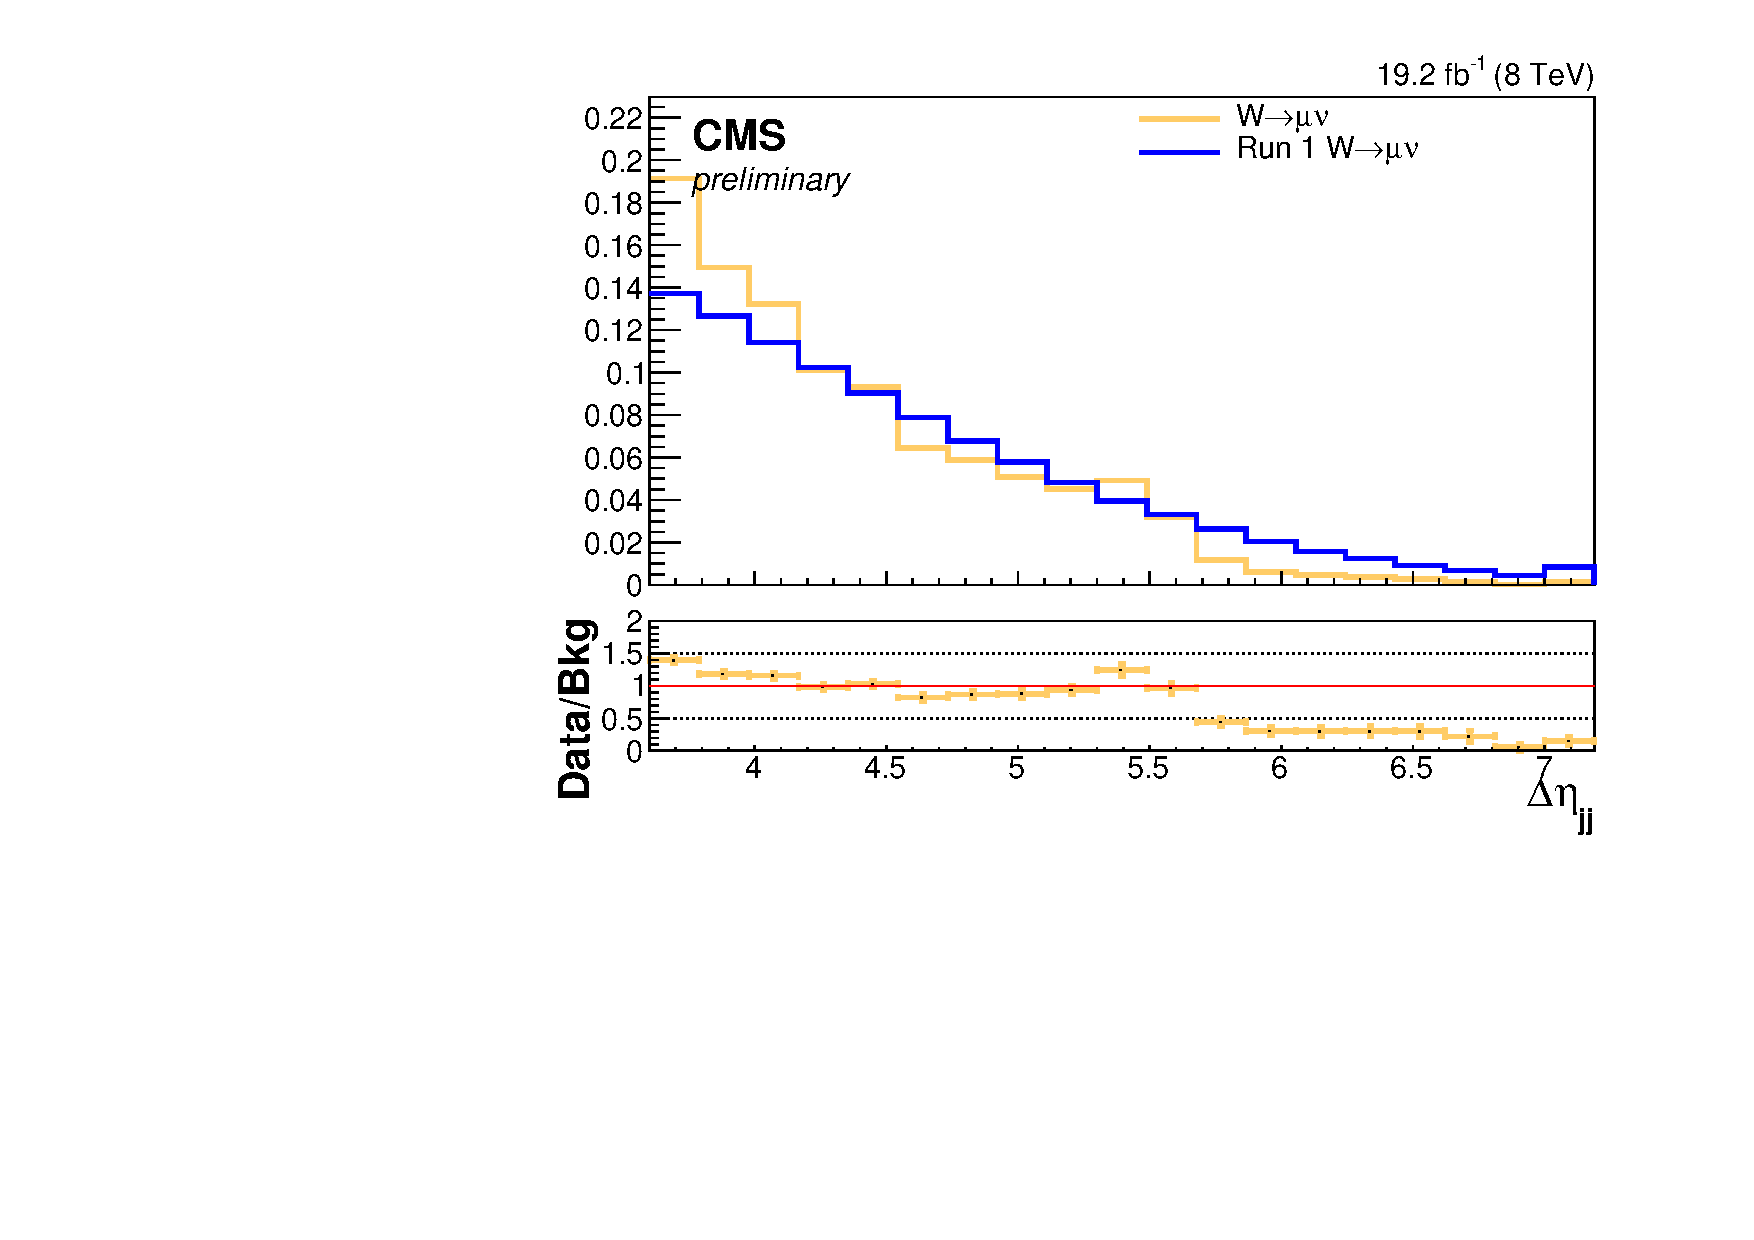
\includegraphics[width=.5\textwidth]{TalkPics/wcontplots090615/output_run1compdynoweight/munu_norm_dijet_deta.pdf}
  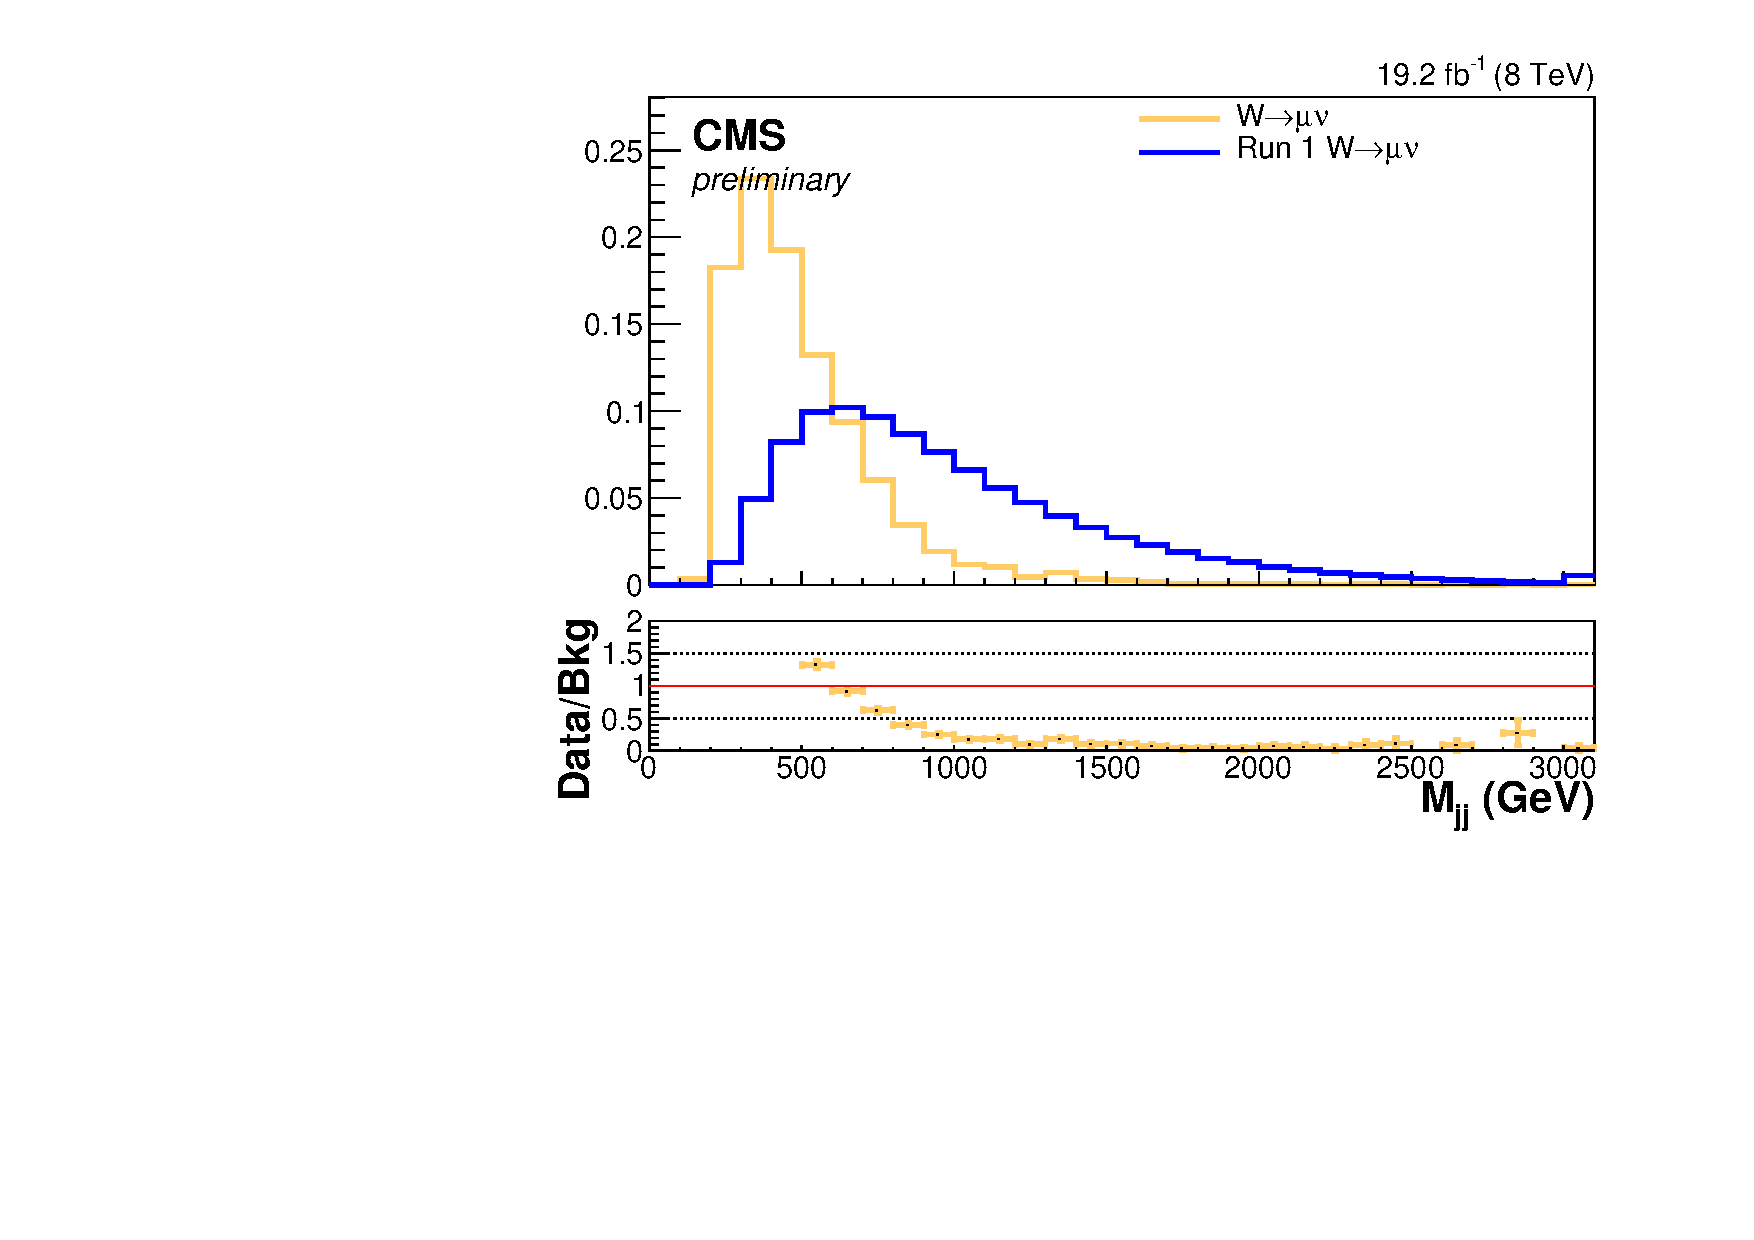
\includegraphics[width=.5\textwidth]{TalkPics/wcontplots090615/output_run1compdynoweight/munu_norm_dijet_M.pdf}
   \begin{block}{}
     \begin{itemize}
     \item Difference could be due to met significance bias
     \end{itemize}
   \end{block}
\end{frame}

\begin{frame}
  \frametitle{W munu Comparison: run 1 vs run 2: N jets}
  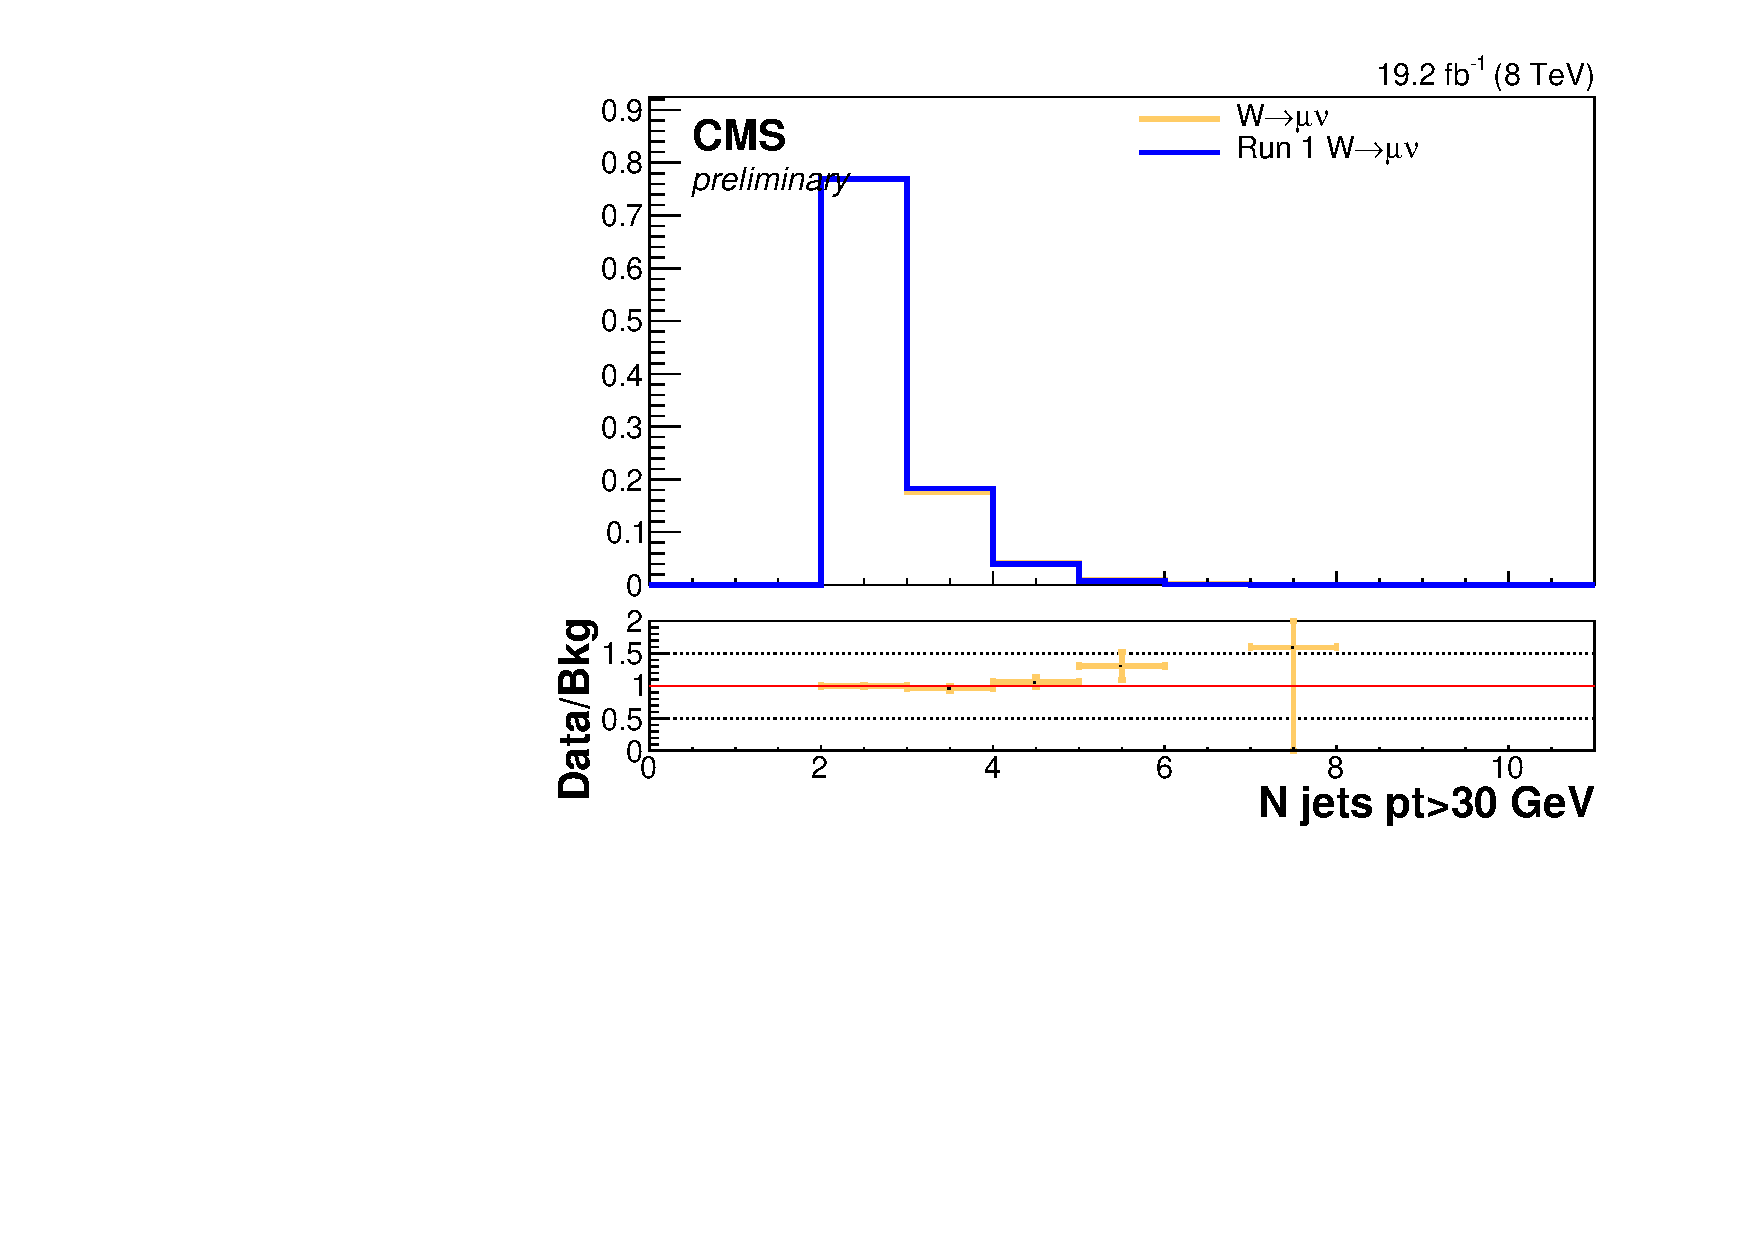
\includegraphics[width=.5\textwidth]{TalkPics/wcontplots090615/output_run1compdynoweight/munu_norm_n_jets_30.pdf}
  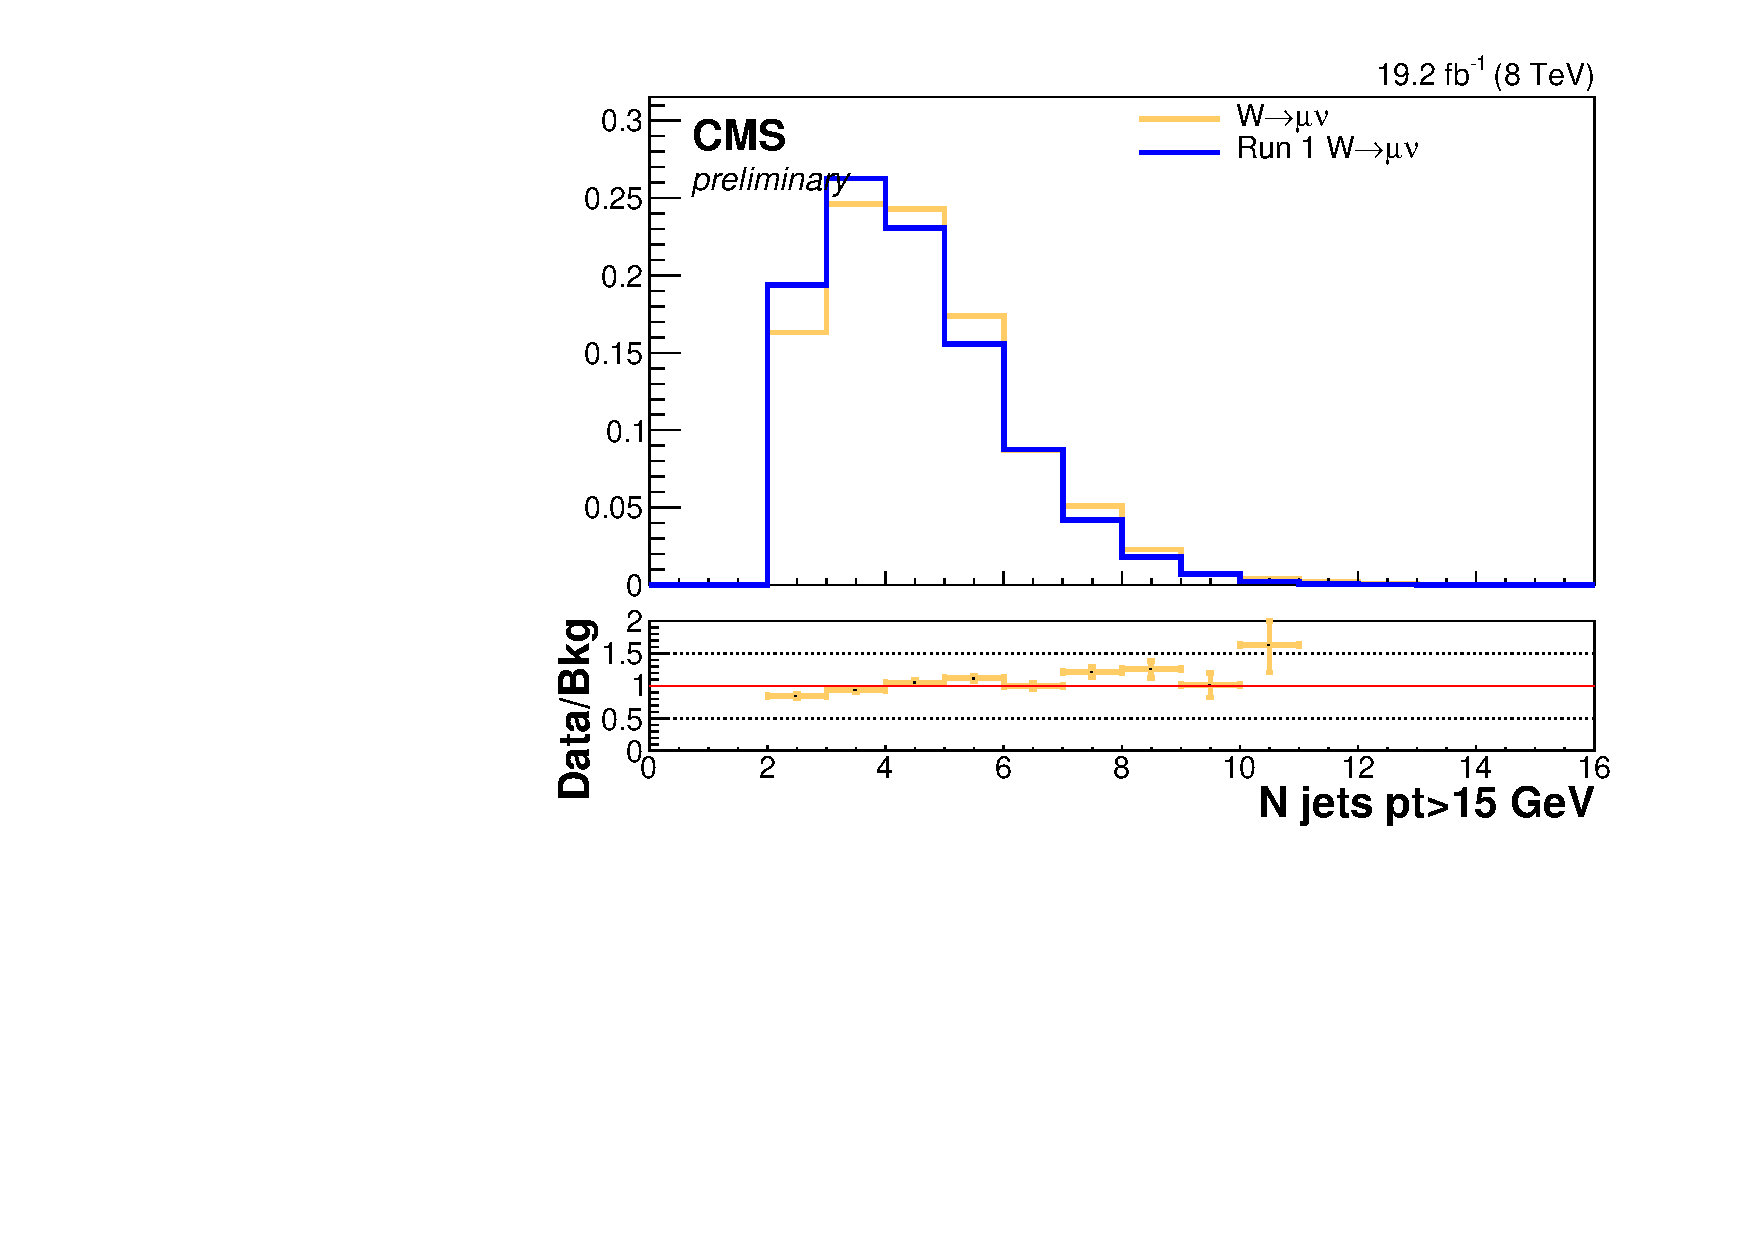
\includegraphics[width=.5\textwidth]{TalkPics/wcontplots090615/output_run1compdynoweight/munu_norm_n_jets_15.pdf}
\end{frame}

\begin{frame}
  \frametitle{W taunu Comparison: run 1 vs run 2: Jet $p_{T}$}
  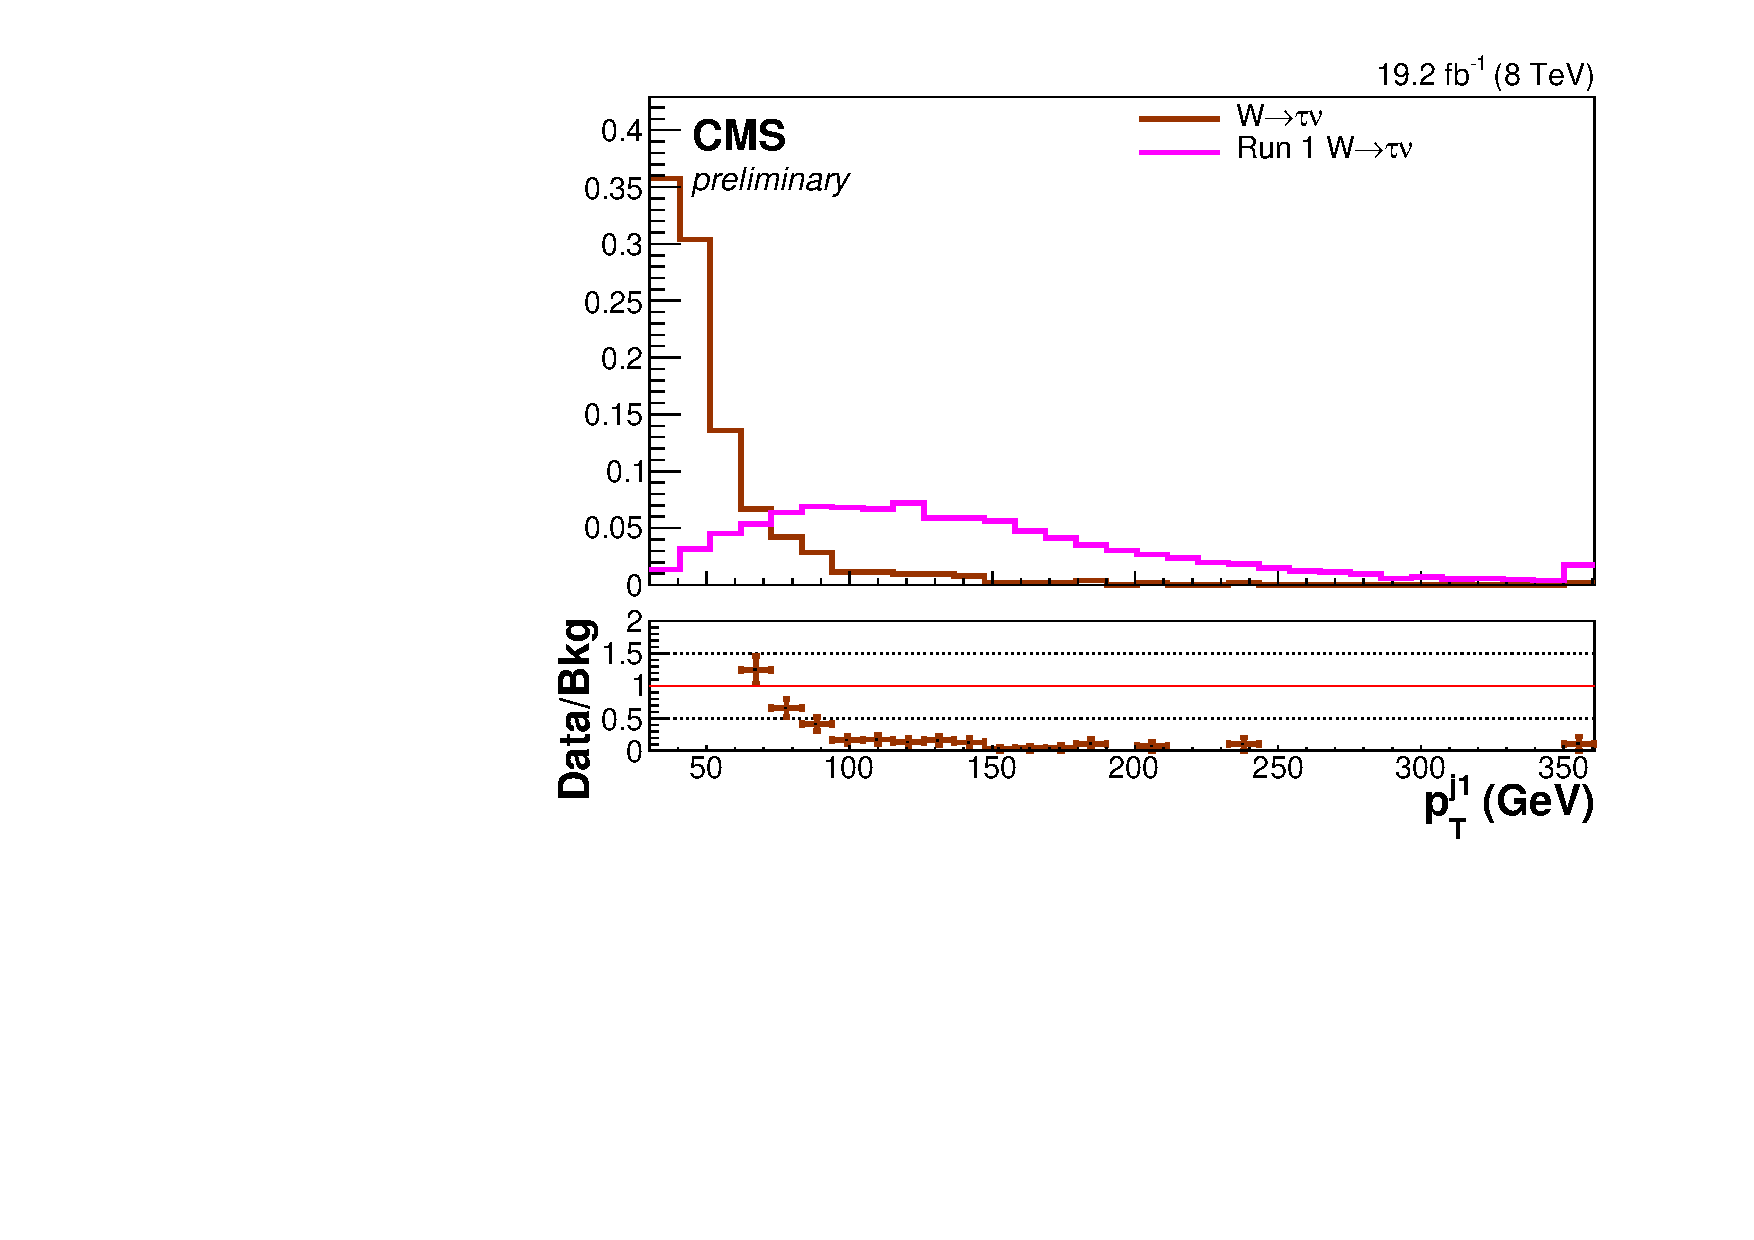
\includegraphics[width=.5\textwidth]{TalkPics/wcontplots090615/output_run1compdynoweight/taunu_norm_jet1_pt.pdf}
  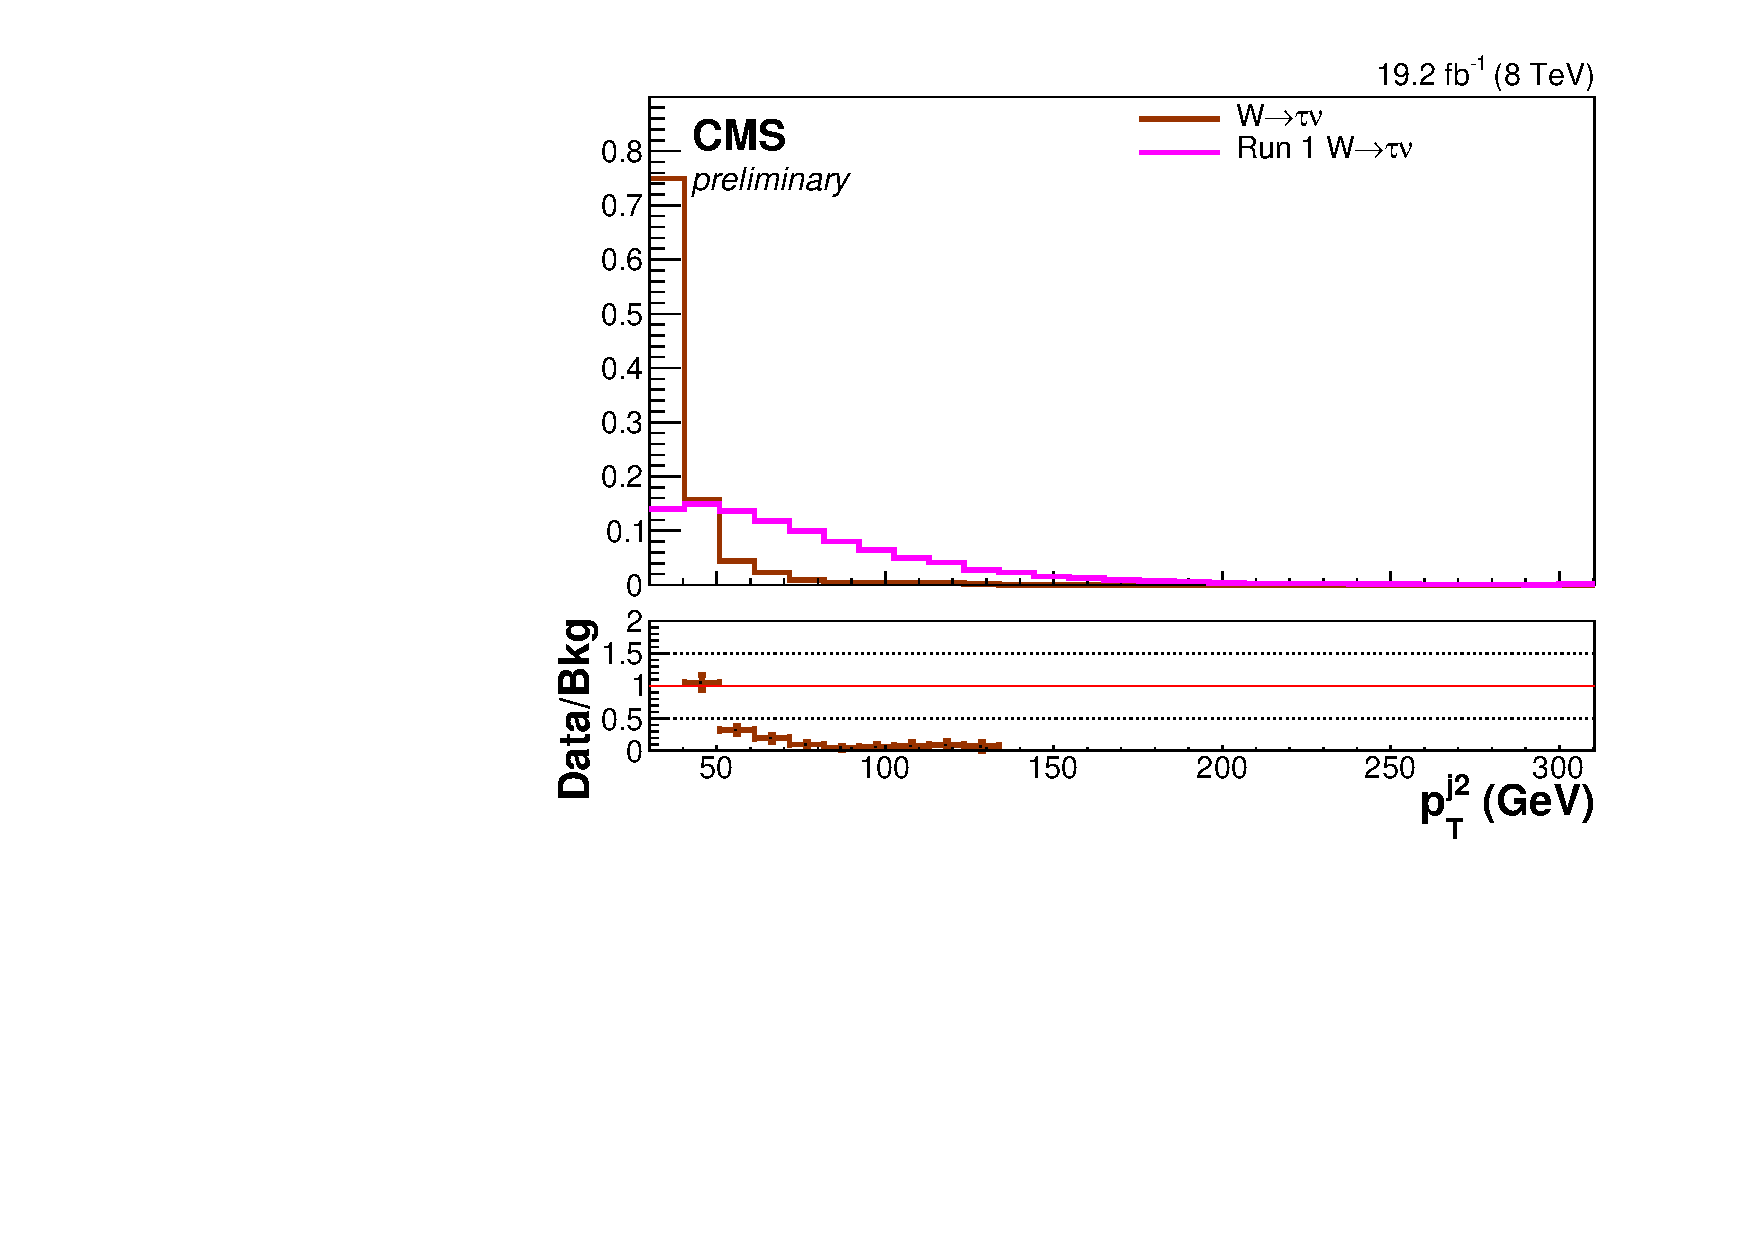
\includegraphics[width=.5\textwidth]{TalkPics/wcontplots090615/output_run1compdynoweight/taunu_norm_jet2_pt.pdf}
  \begin{block}{}
    \begin{itemize}
    \item Same as enu and munu
    \end{itemize}
  \end{block}
\end{frame}

\begin{frame}
  \frametitle{W taunu Comparison: run 1 vs run 2: Jet $\eta$}
  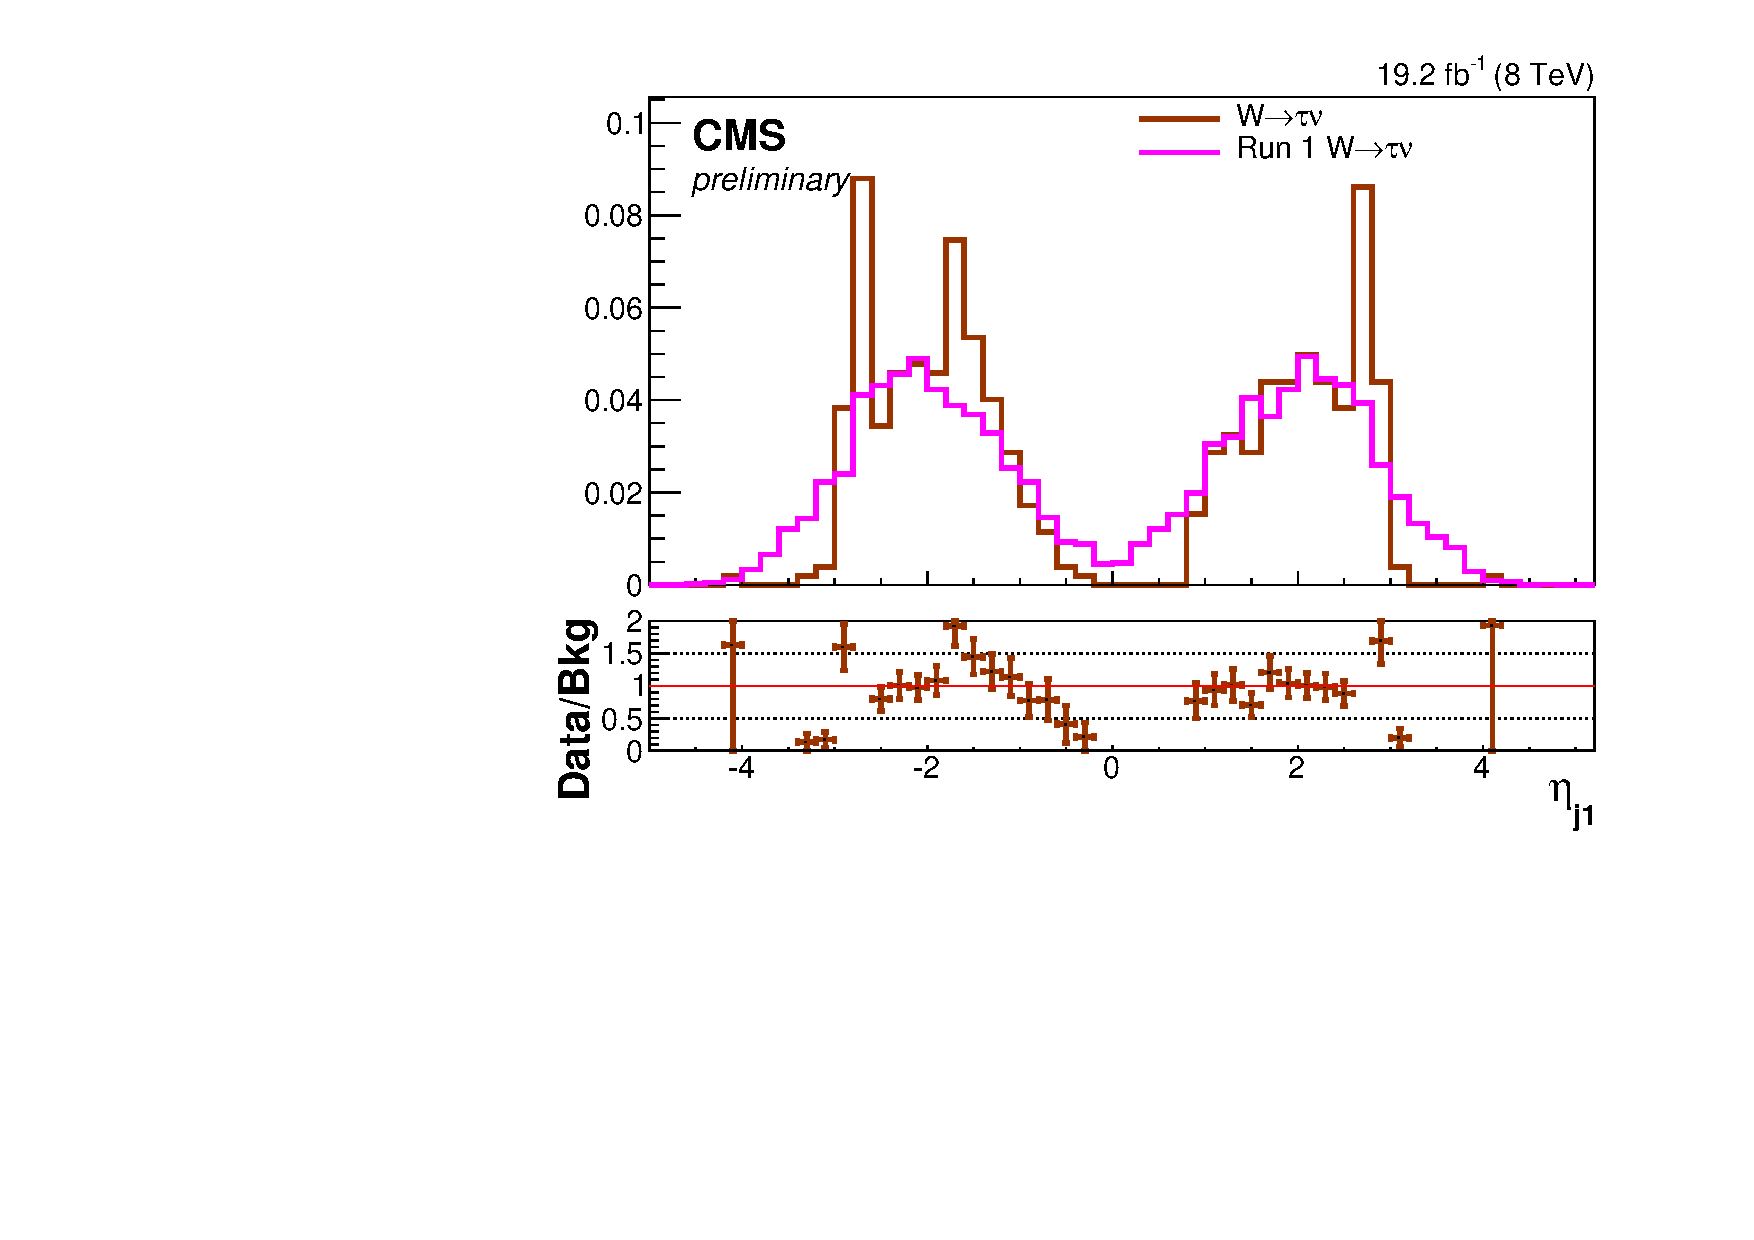
\includegraphics[width=.5\textwidth]{TalkPics/wcontplots090615/output_run1compdynoweight/taunu_norm_jet1_eta.pdf}
  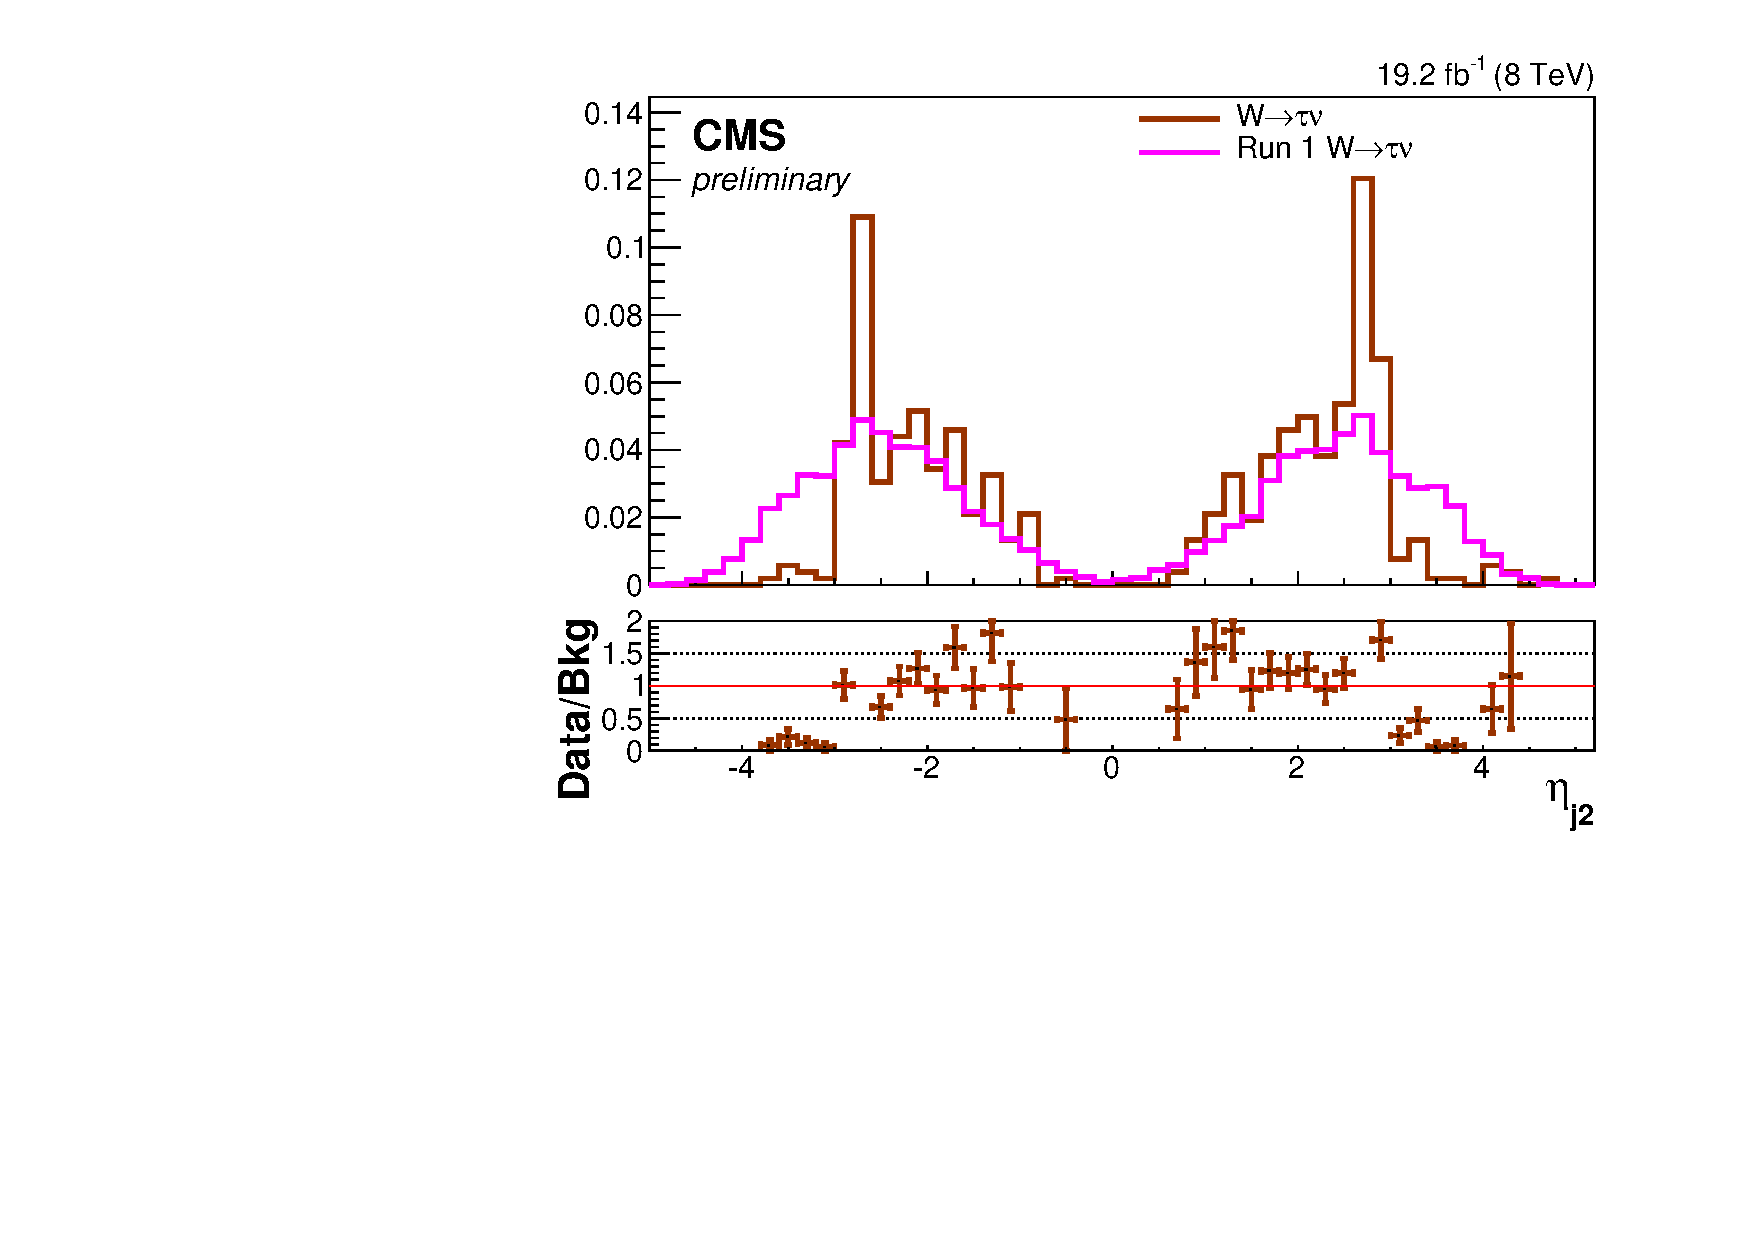
\includegraphics[width=.5\textwidth]{TalkPics/wcontplots090615/output_run1compdynoweight/taunu_norm_jet2_eta.pdf}
  \begin{block}{}
    \begin{itemize}
    \item Ears still apparent
    \end{itemize}
  \end{block}
\end{frame}

\begin{frame}
  \frametitle{W taunu Comparison: run 1 vs run 2: Jet $\phi$}
  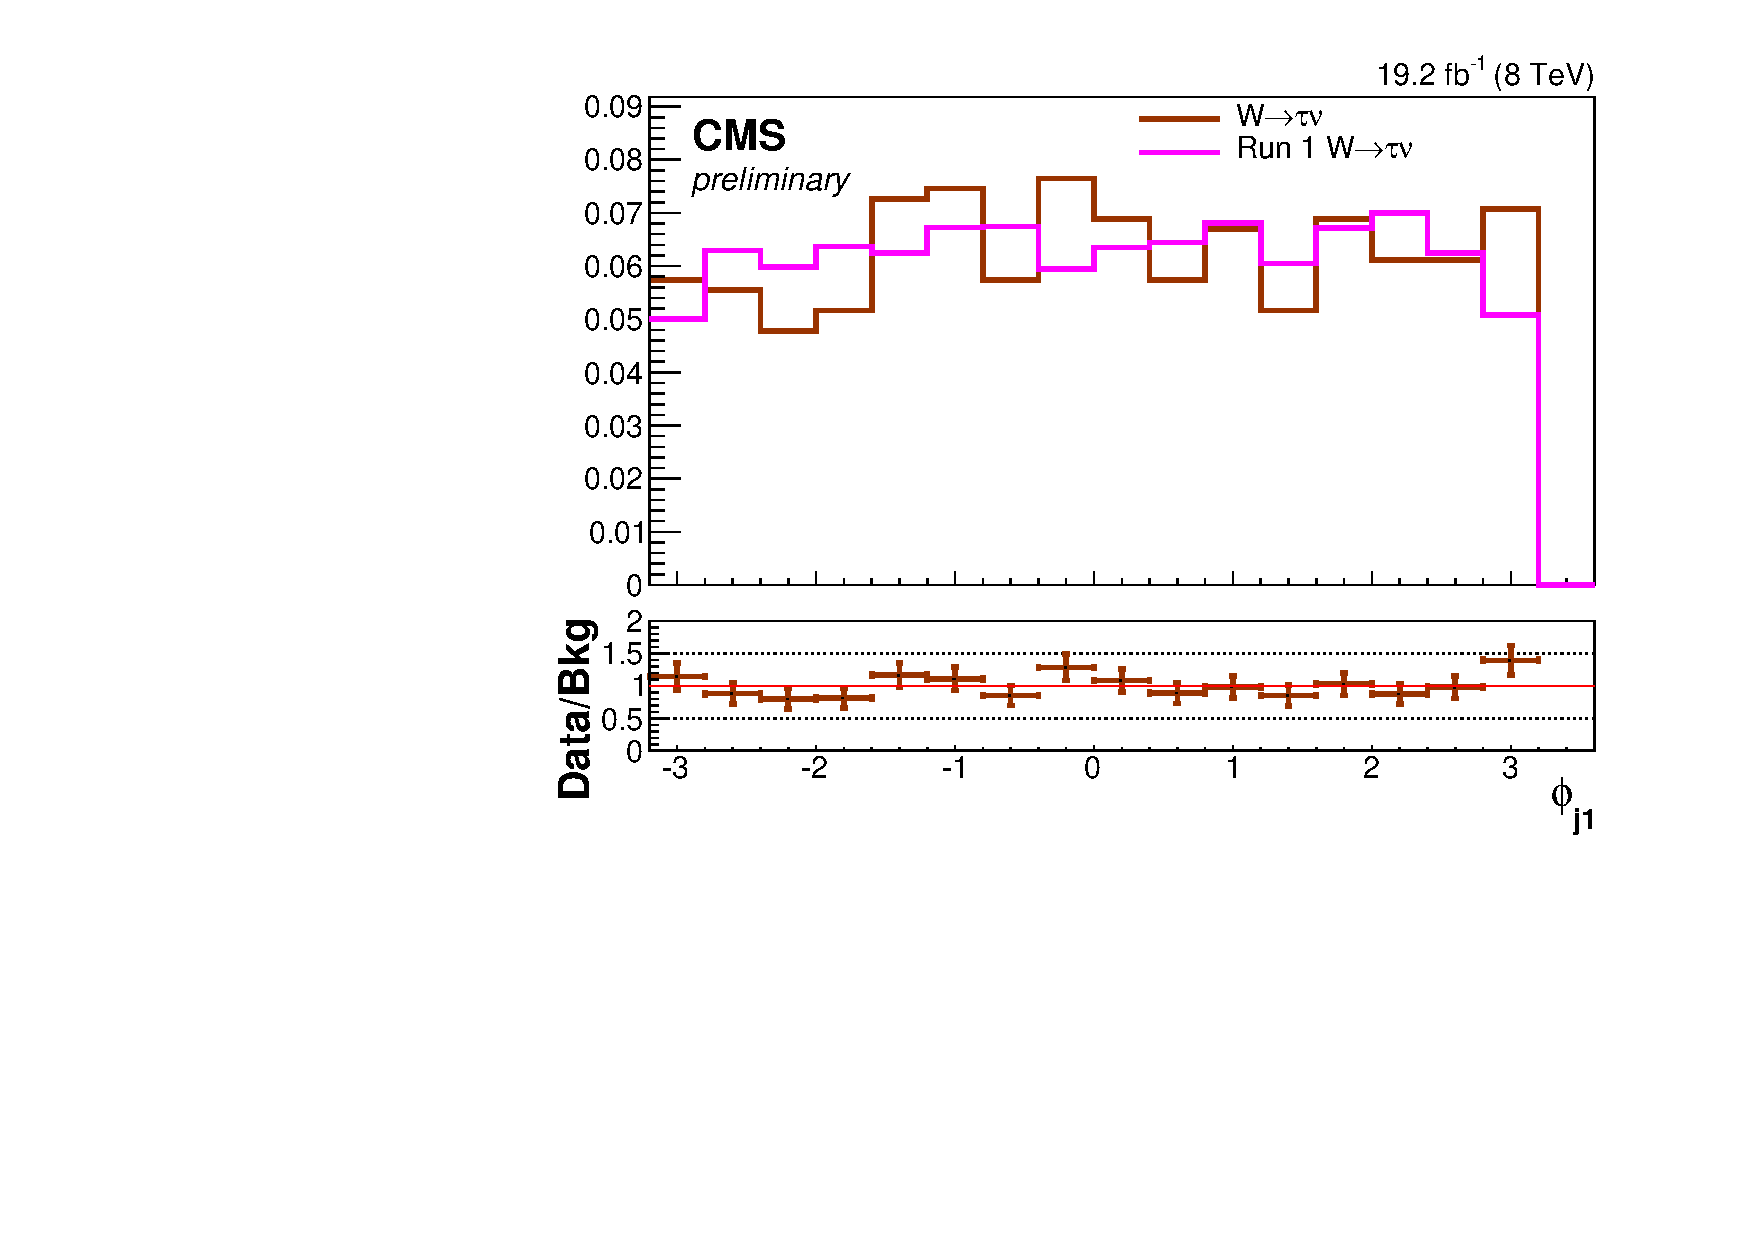
\includegraphics[width=.5\textwidth]{TalkPics/wcontplots090615/output_run1compdynoweight/taunu_norm_jet1_phi.pdf}
  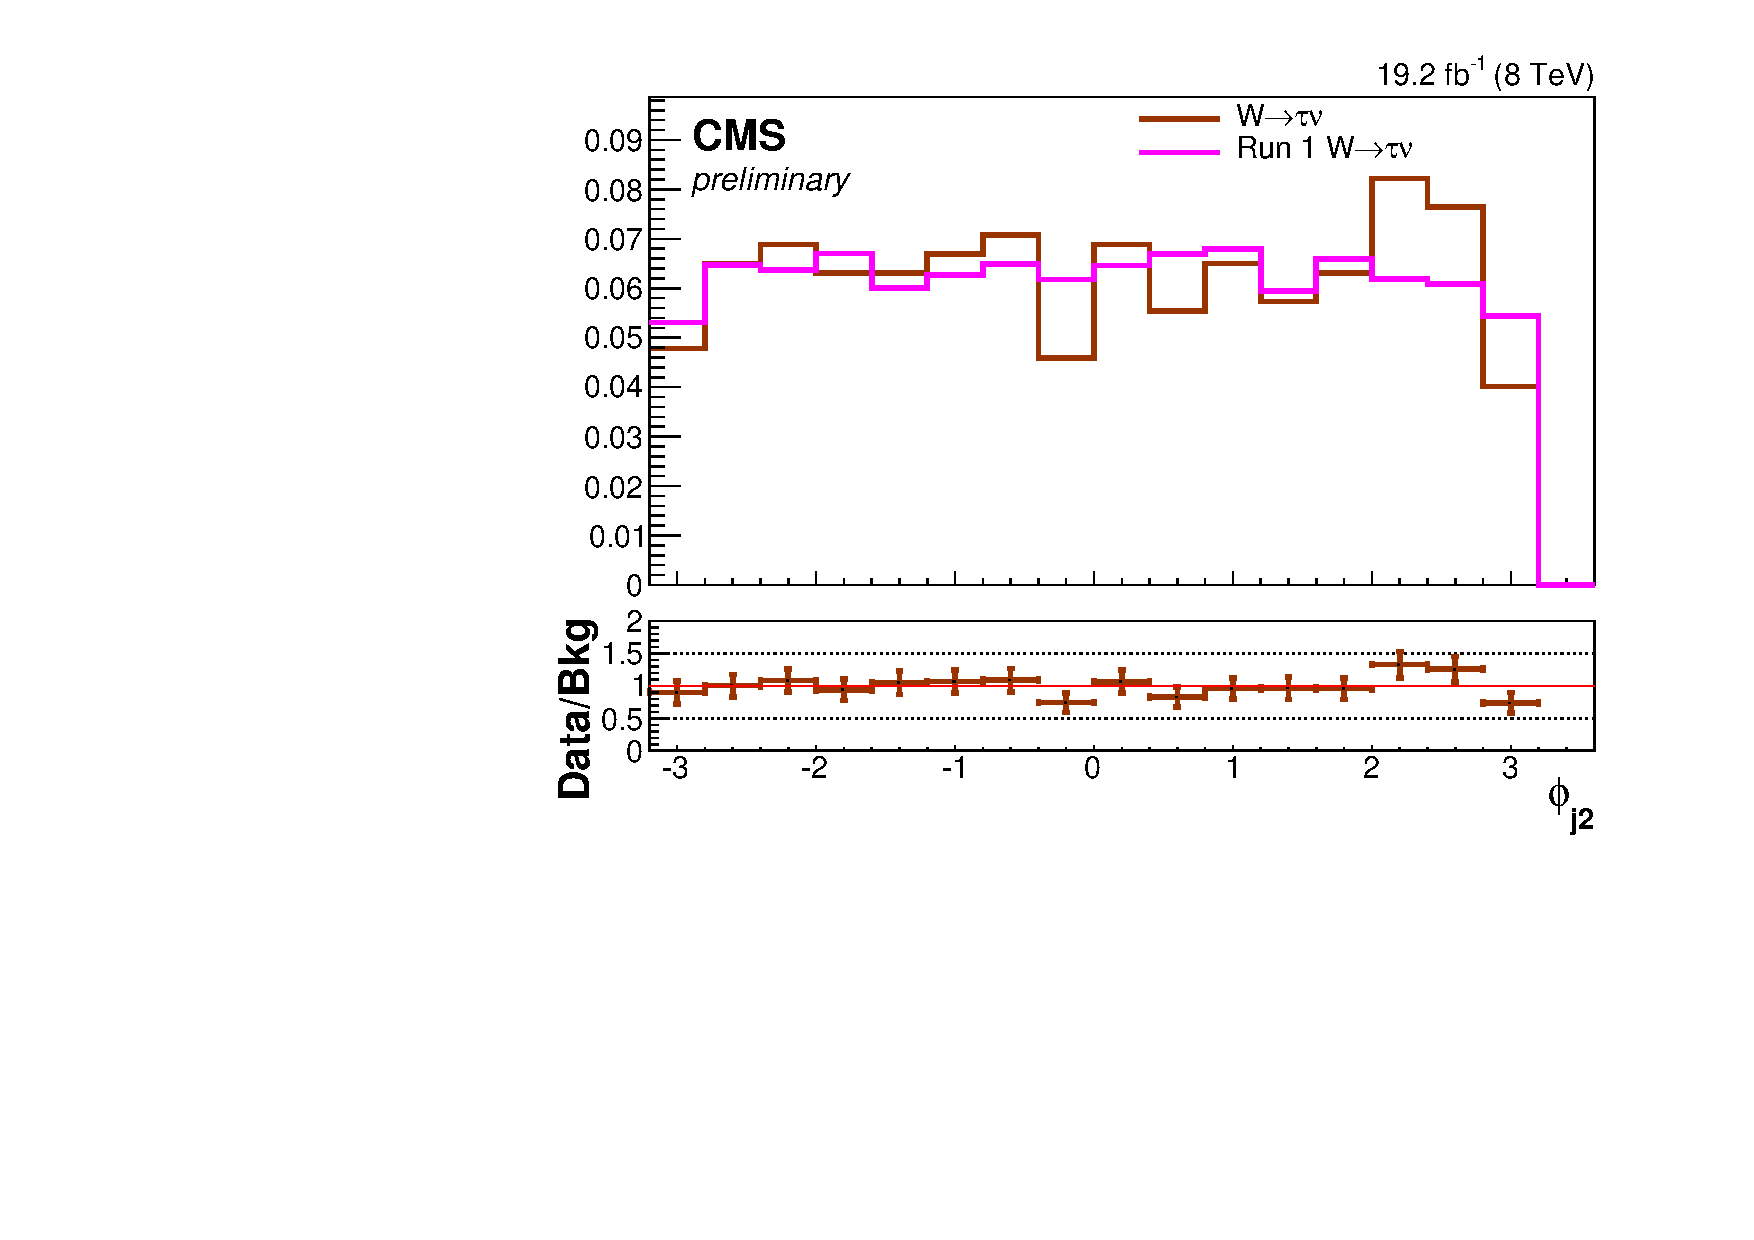
\includegraphics[width=.5\textwidth]{TalkPics/wcontplots090615/output_run1compdynoweight/taunu_norm_jet2_phi.pdf}
  \begin{block}{}
    \begin{itemize}
    \item $\phi$ distributions look similar within stat error
    \end{itemize}
  \end{block}
\end{frame}

\begin{frame}
  \frametitle{W taunu Comparison: run 1 vs run 2: Met}
  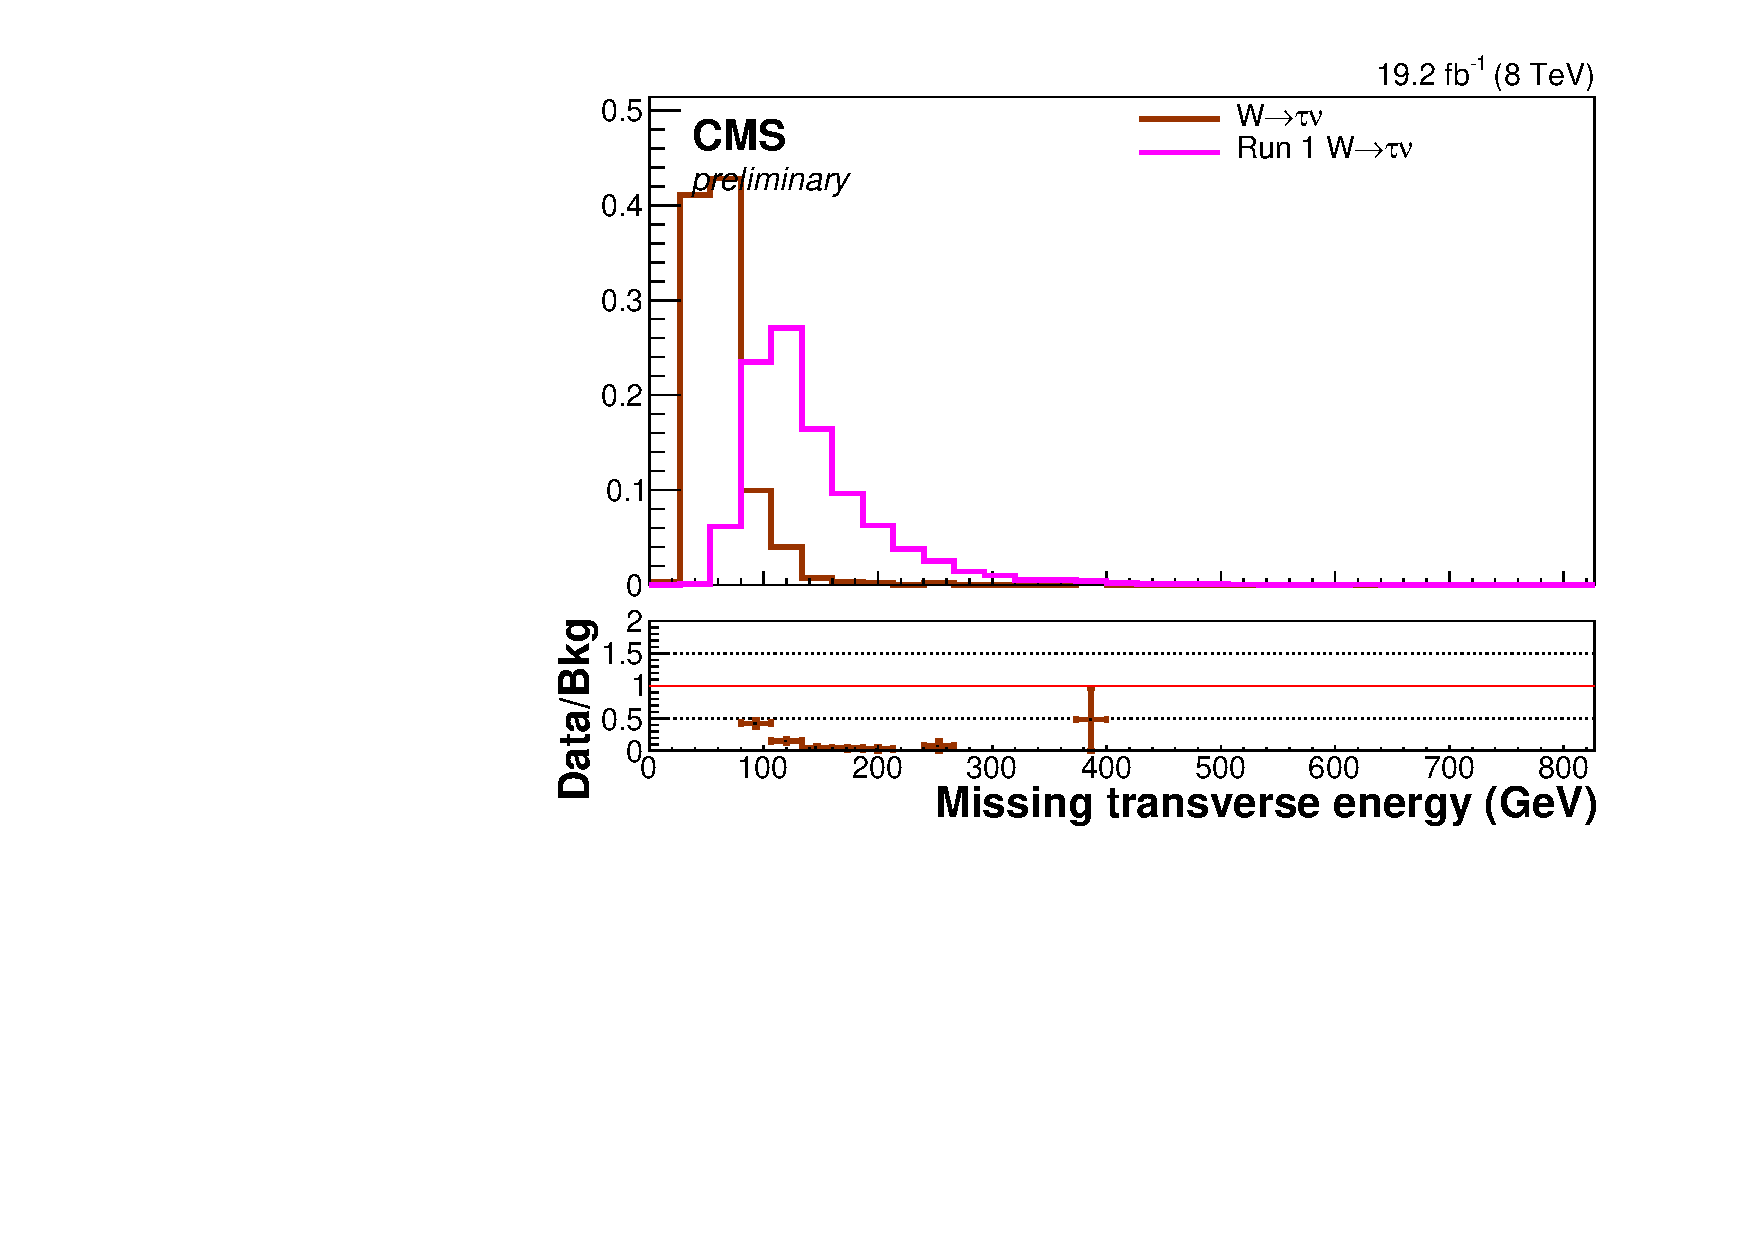
\includegraphics[width=.5\textwidth]{TalkPics/wcontplots090615/output_run1compdynoweight/taunu_norm_metnomuons.pdf}
  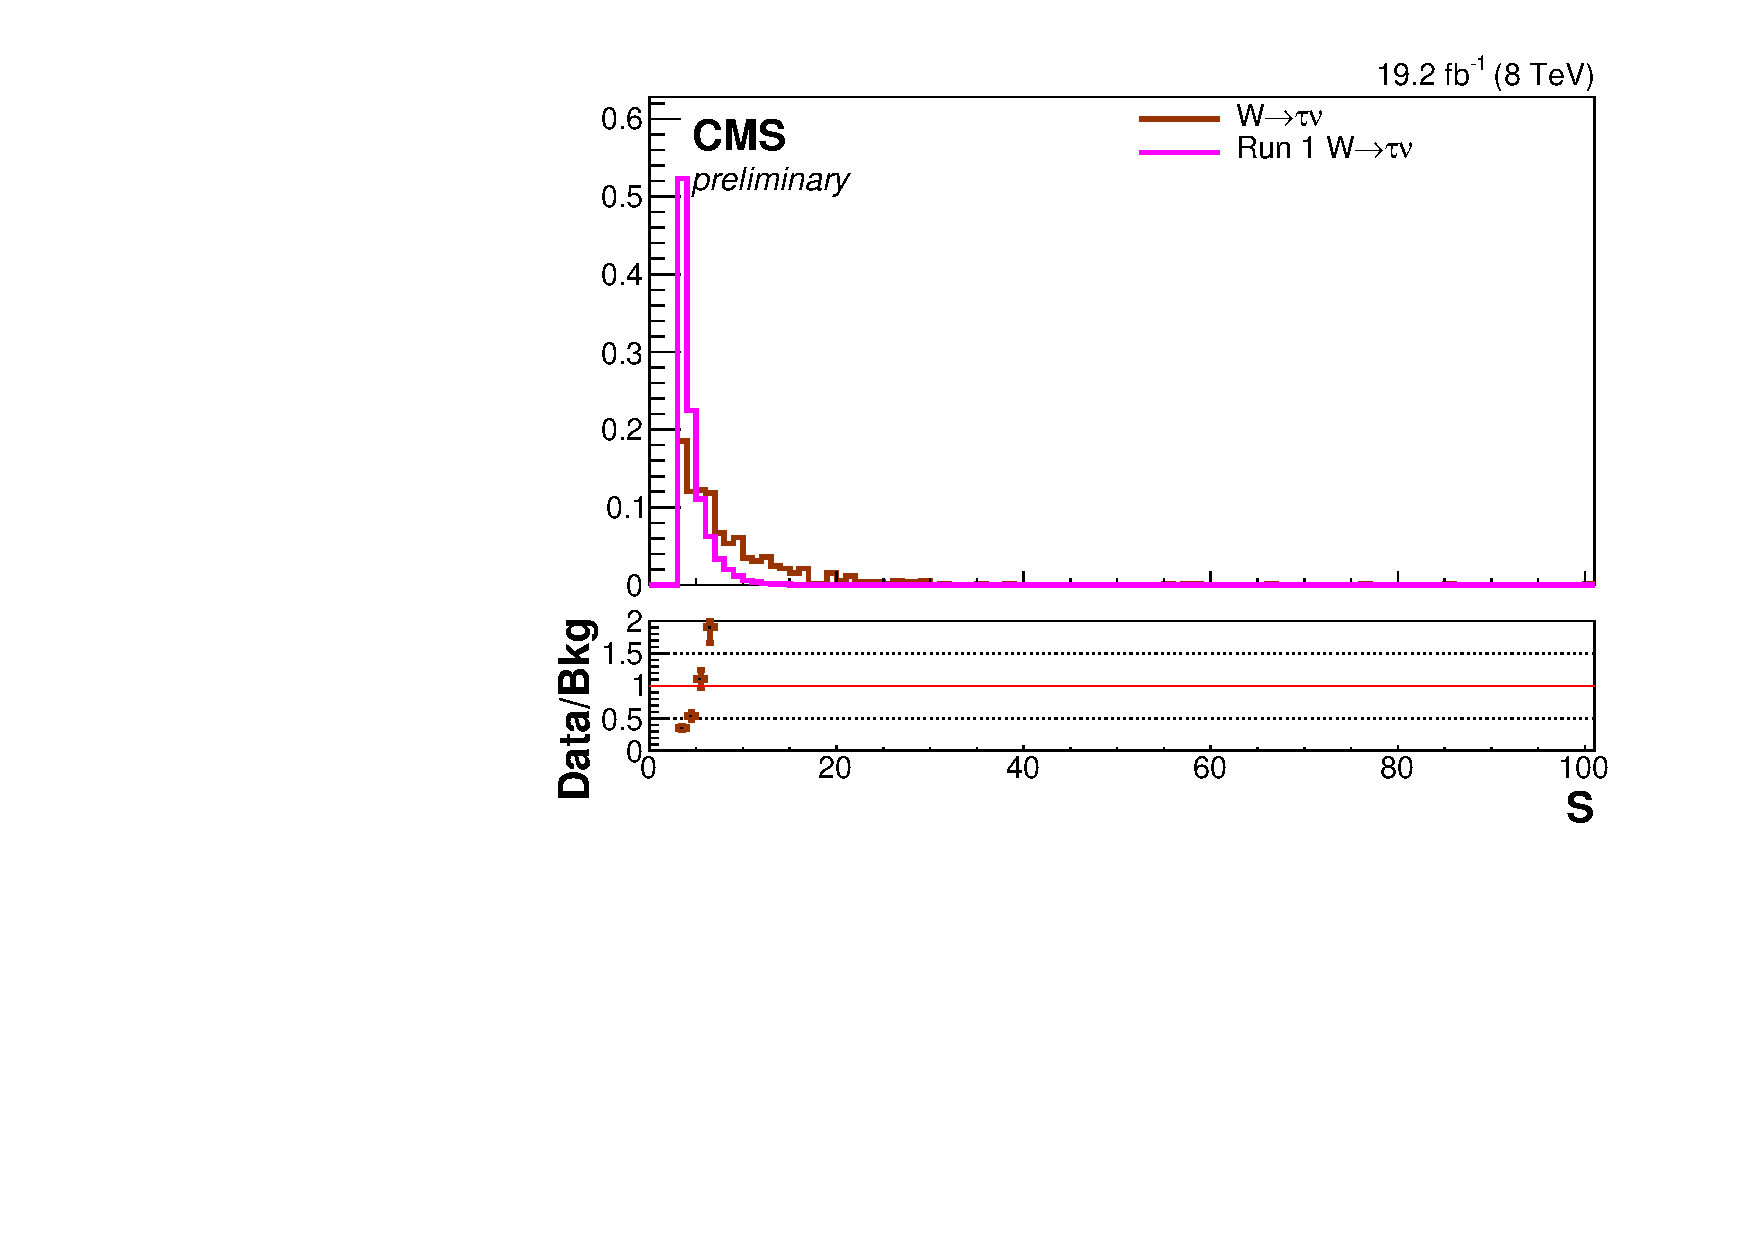
\includegraphics[width=.5\textwidth]{TalkPics/wcontplots090615/output_run1compdynoweight/taunu_norm_metnomu_significance.pdf}
  \begin{block}{}
    \begin{itemize}
    \item Metnomu lower for run 2
    \item Met significance is a different variable in miniAOD to the one we used in run 1
    \end{itemize}
  \end{block}
\end{frame}

\begin{frame}
  \frametitle{W taunu Comparison: run 1 vs run 2: $\Delta\phi$ variables}
  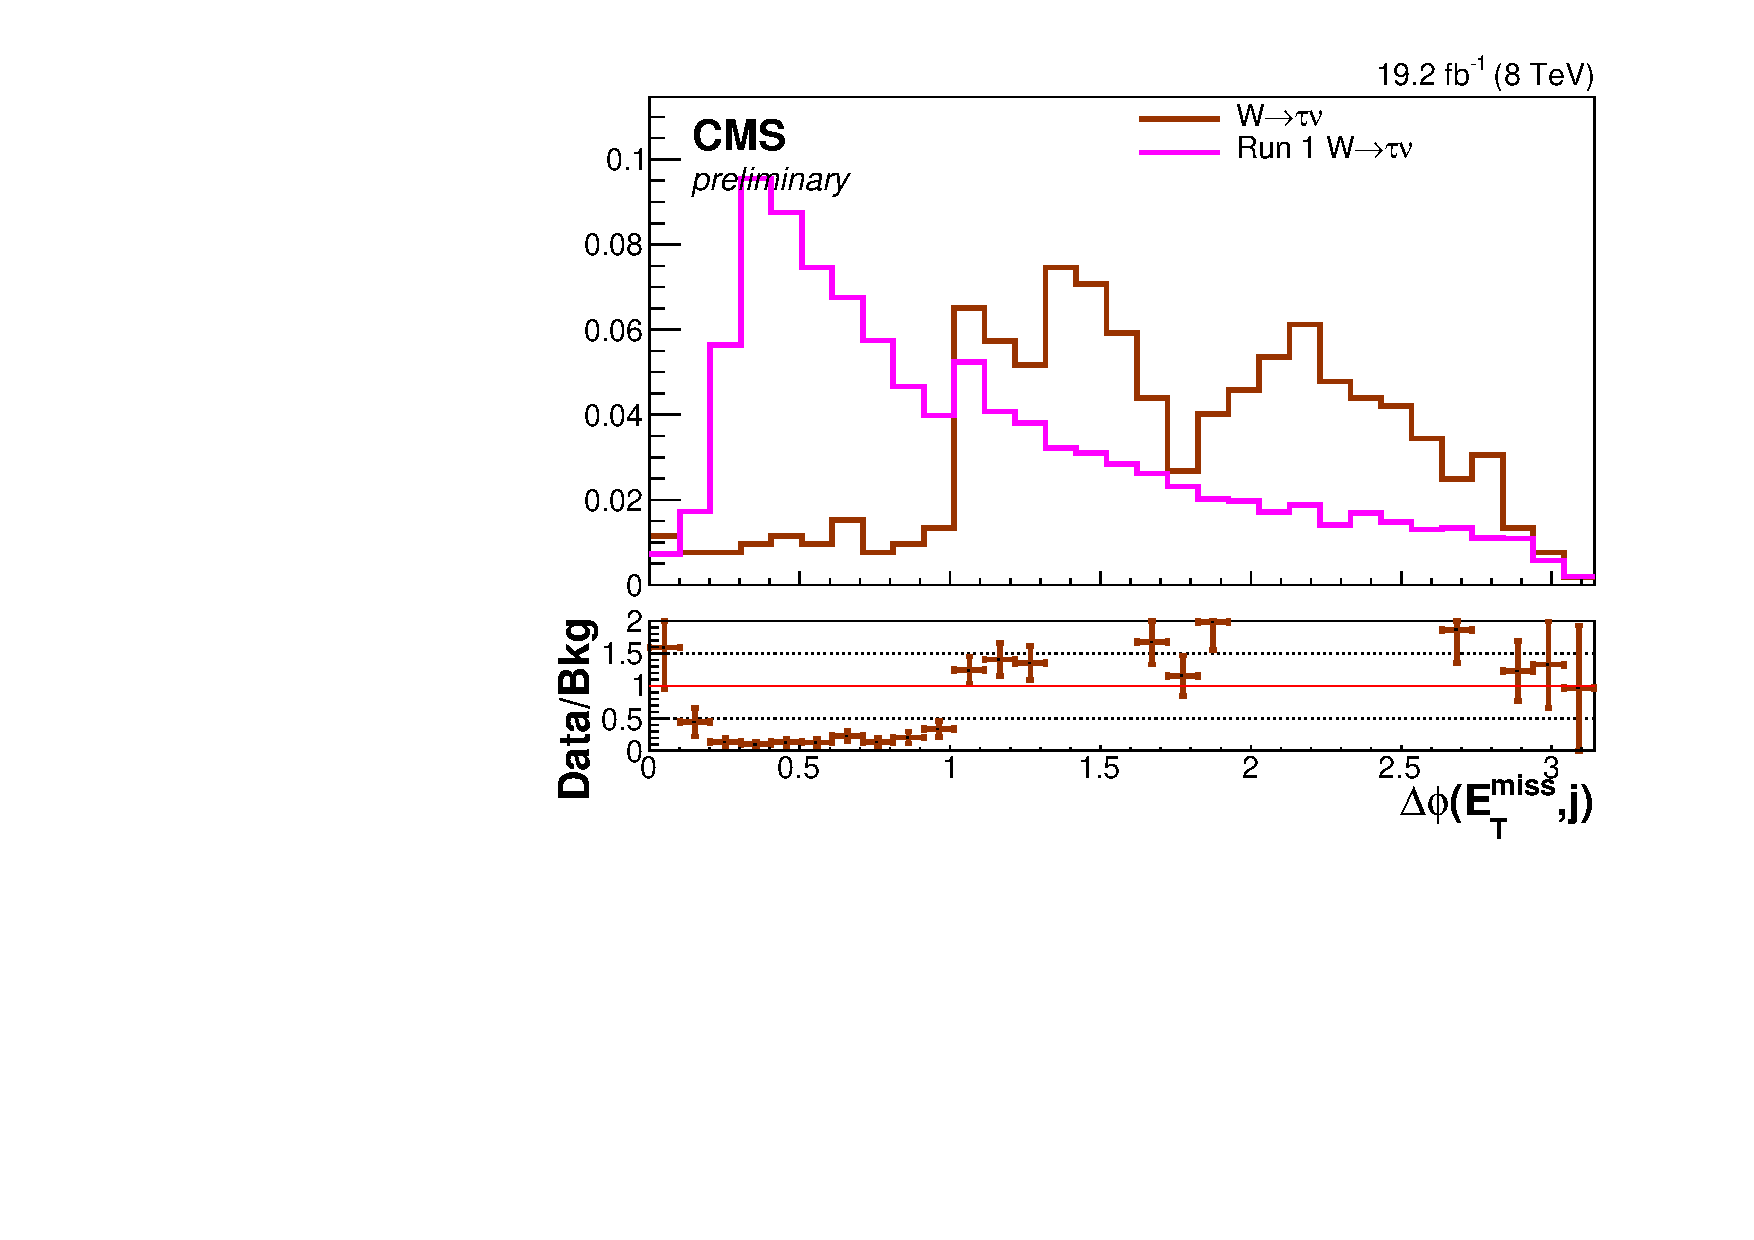
\includegraphics[width=.5\textwidth]{TalkPics/wcontplots090615/output_run1compdynoweight/taunu_norm_alljetsmetnomu_mindphi.pdf}
  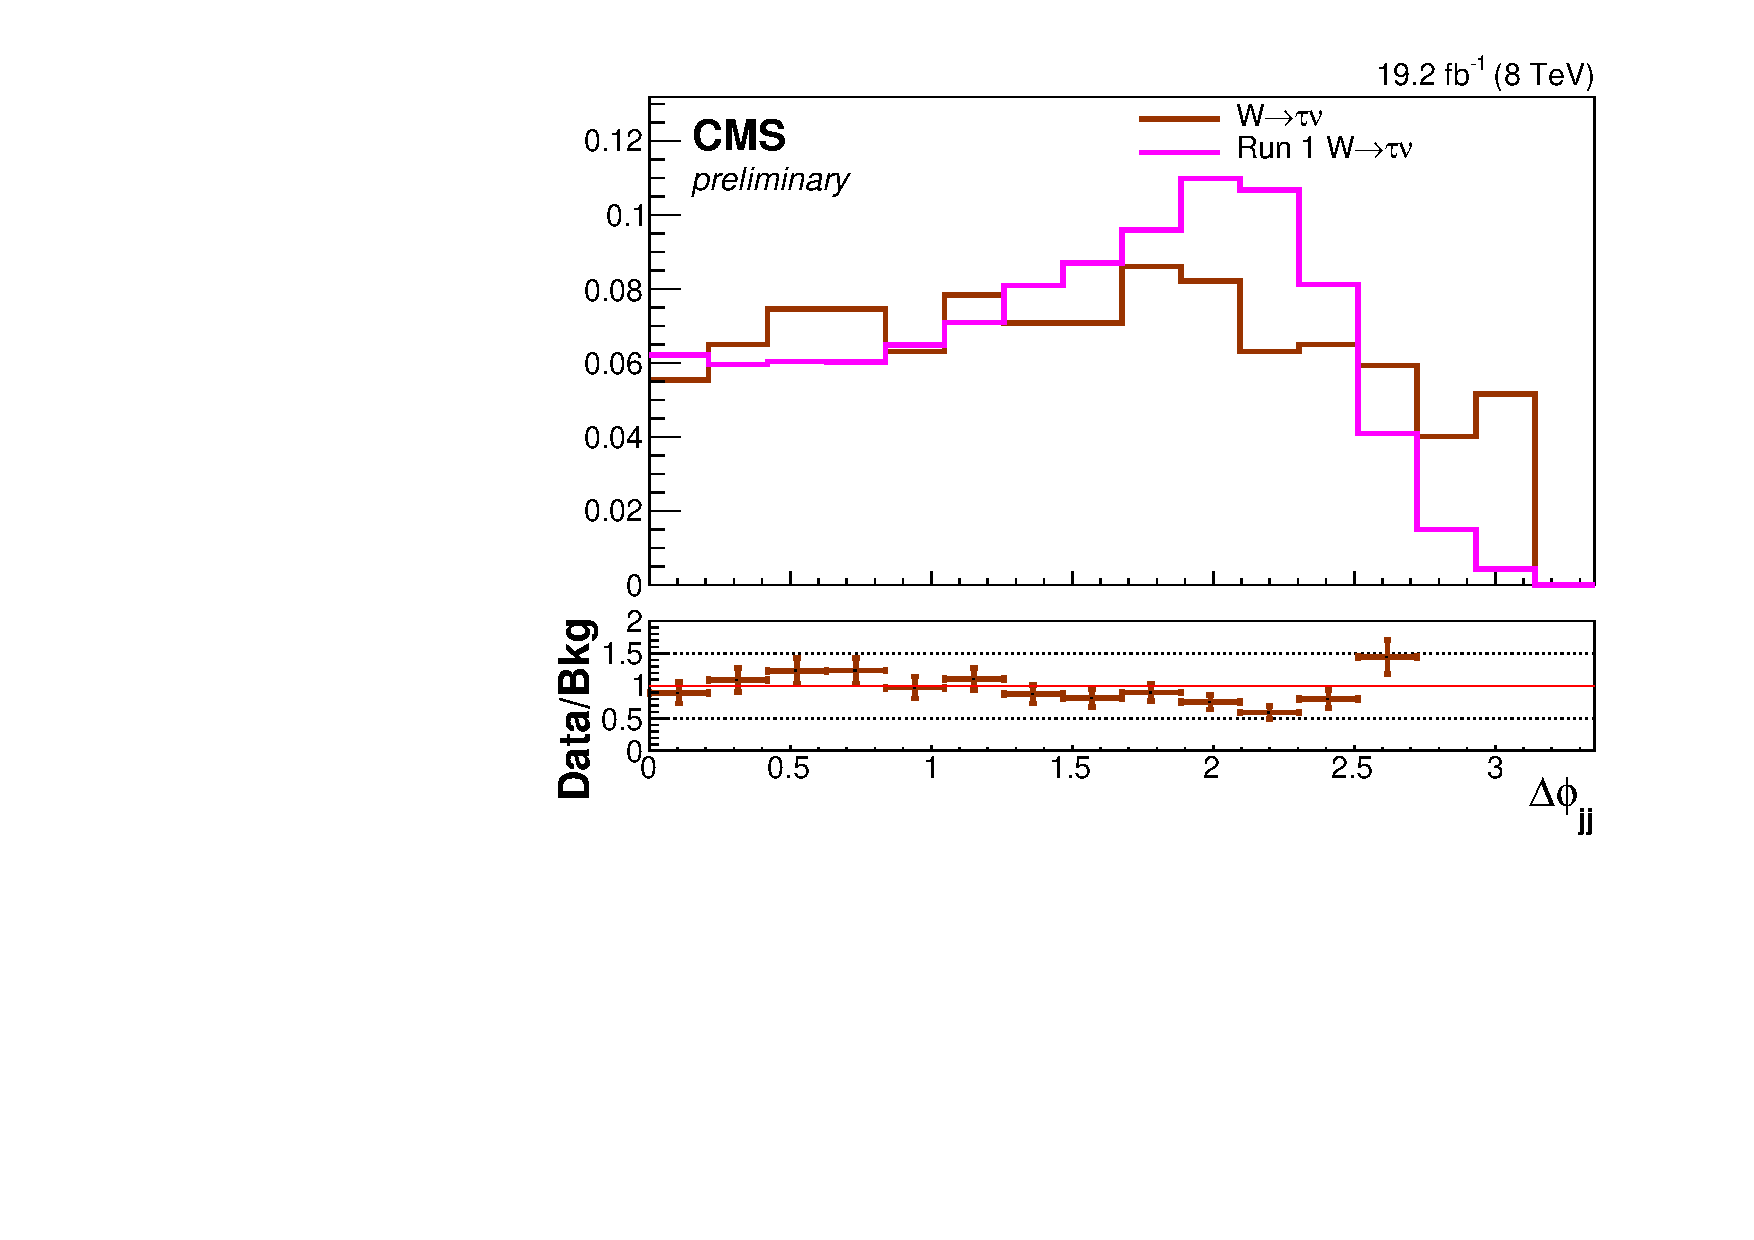
\includegraphics[width=.5\textwidth]{TalkPics/wcontplots090615/output_run1compdynoweight/taunu_norm_dijet_dphi.pdf}
  \begin{block}{}
    \begin{itemize}
    \item Step effect in left plot due to cut on leading jets met dphi in tau category
    \end{itemize}
  \end{block}
\end{frame}

\begin{frame}
  \frametitle{W taunu Comparison: run 1 vs run 2: dijet variables}
  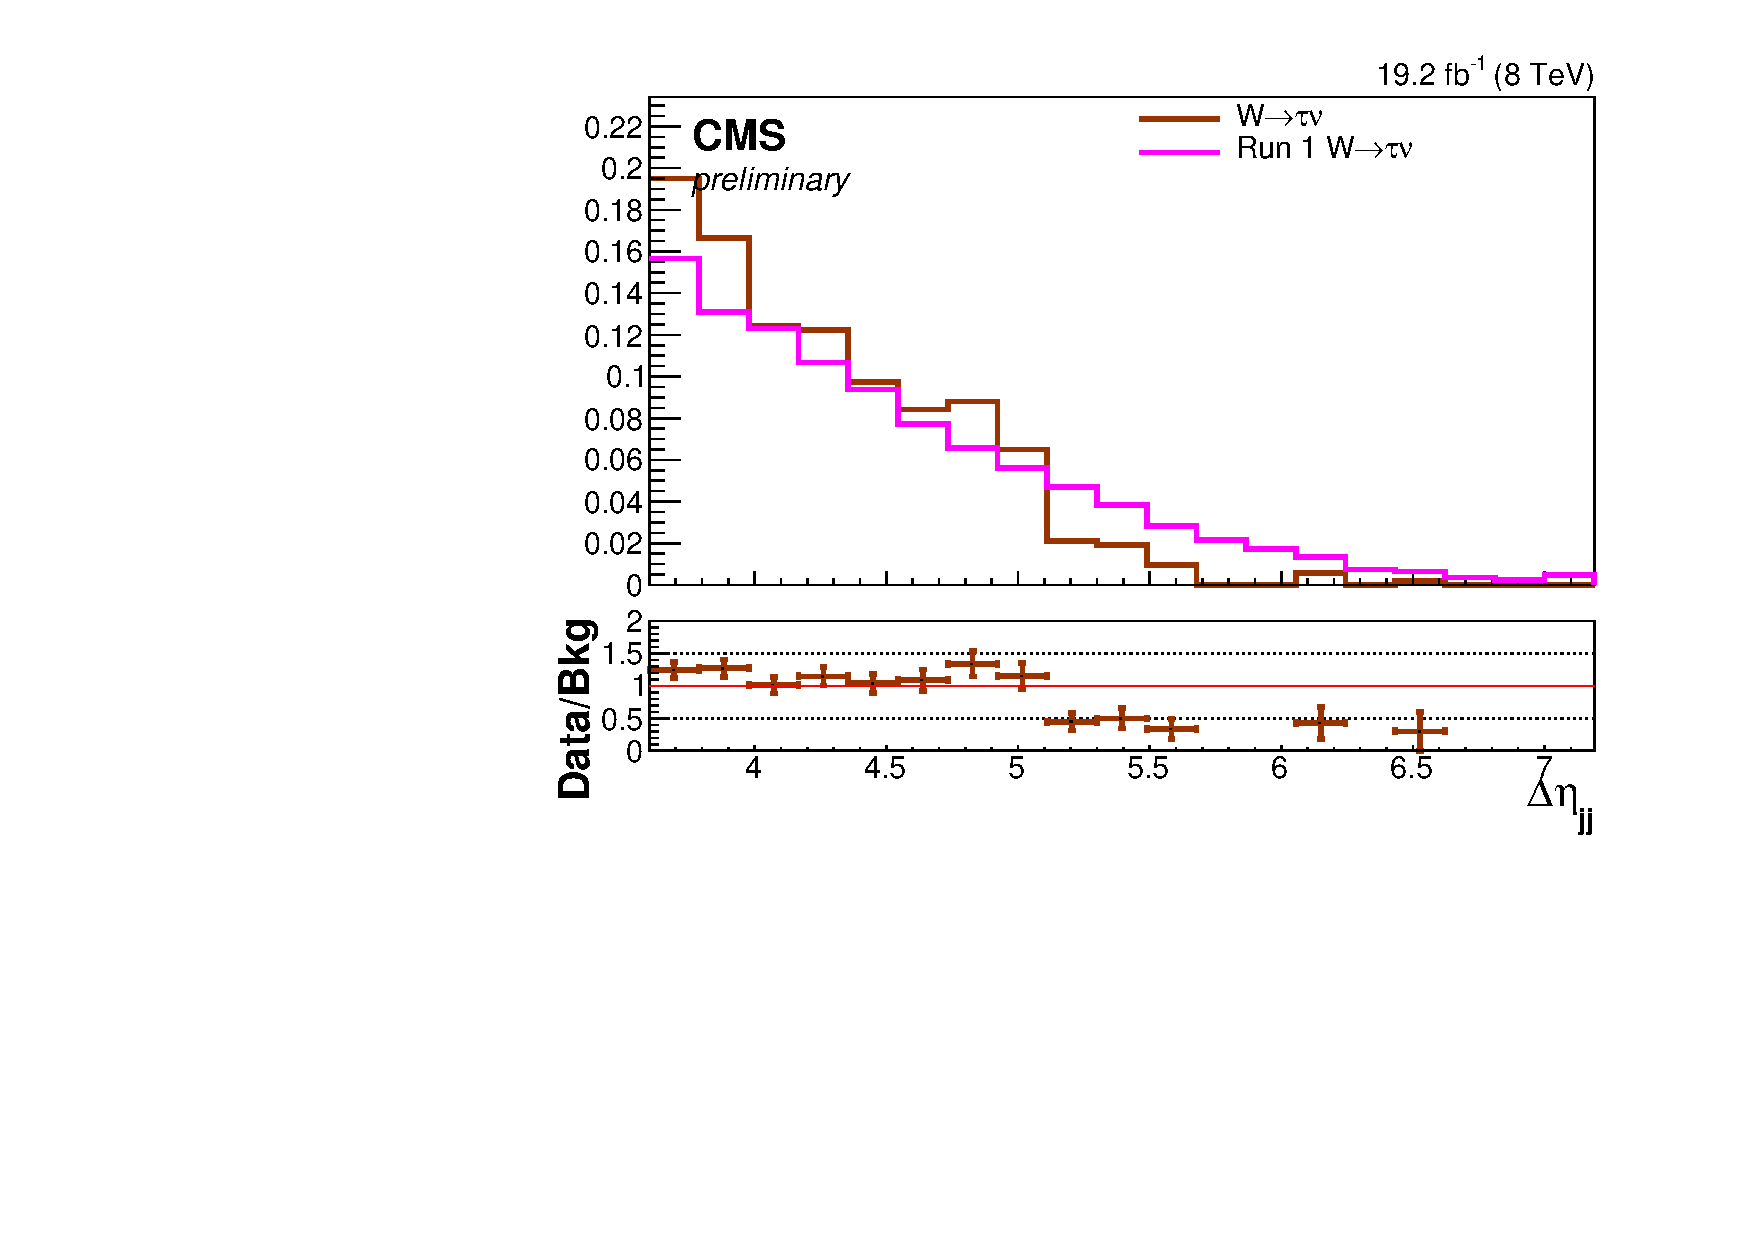
\includegraphics[width=.5\textwidth]{TalkPics/wcontplots090615/output_run1compdynoweight/taunu_norm_dijet_deta.pdf}
  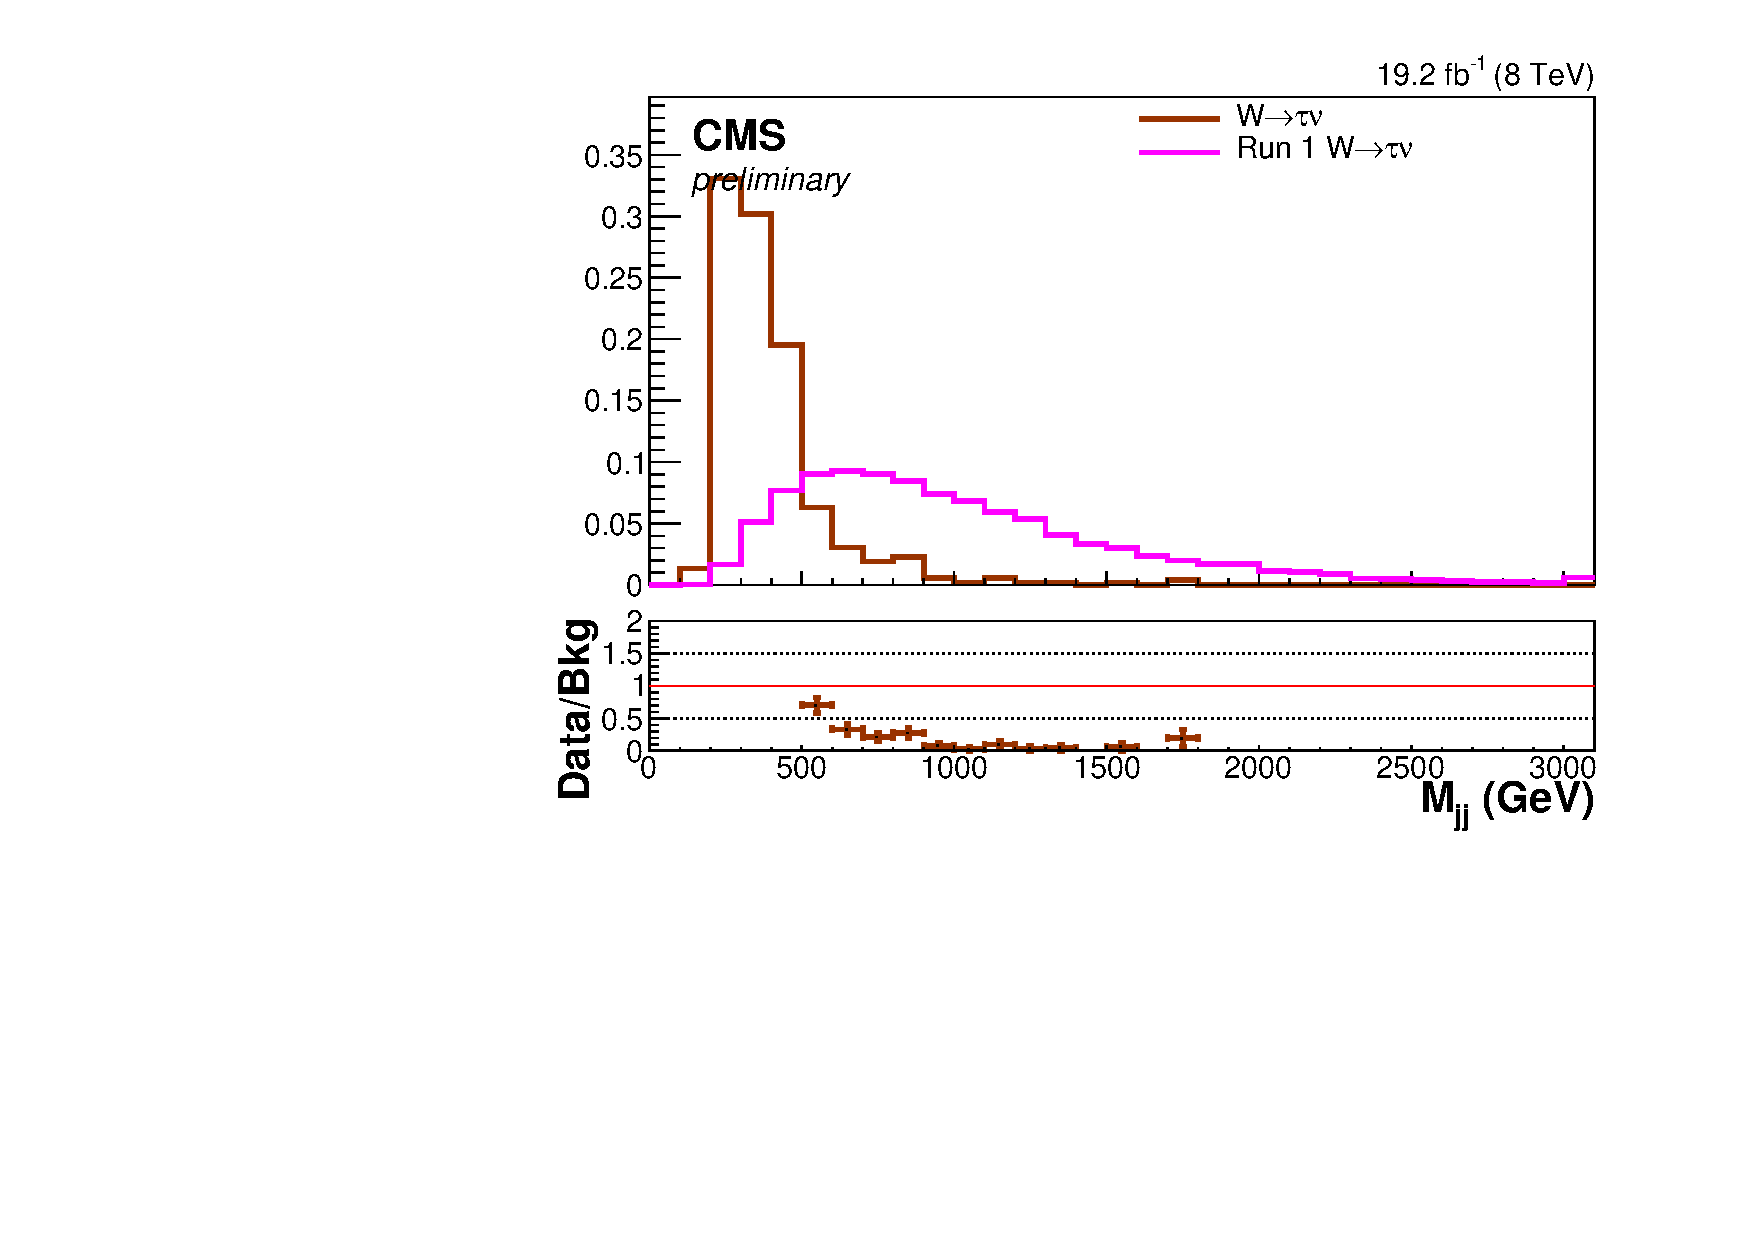
\includegraphics[width=.5\textwidth]{TalkPics/wcontplots090615/output_run1compdynoweight/taunu_norm_dijet_M.pdf}
   \begin{block}{}
     \begin{itemize}
     \item Could be due to met significance cut
     \end{itemize}
   \end{block}
\end{frame}

\begin{frame}
  \frametitle{W Comparison: run 1 vs run 2: N jets}
  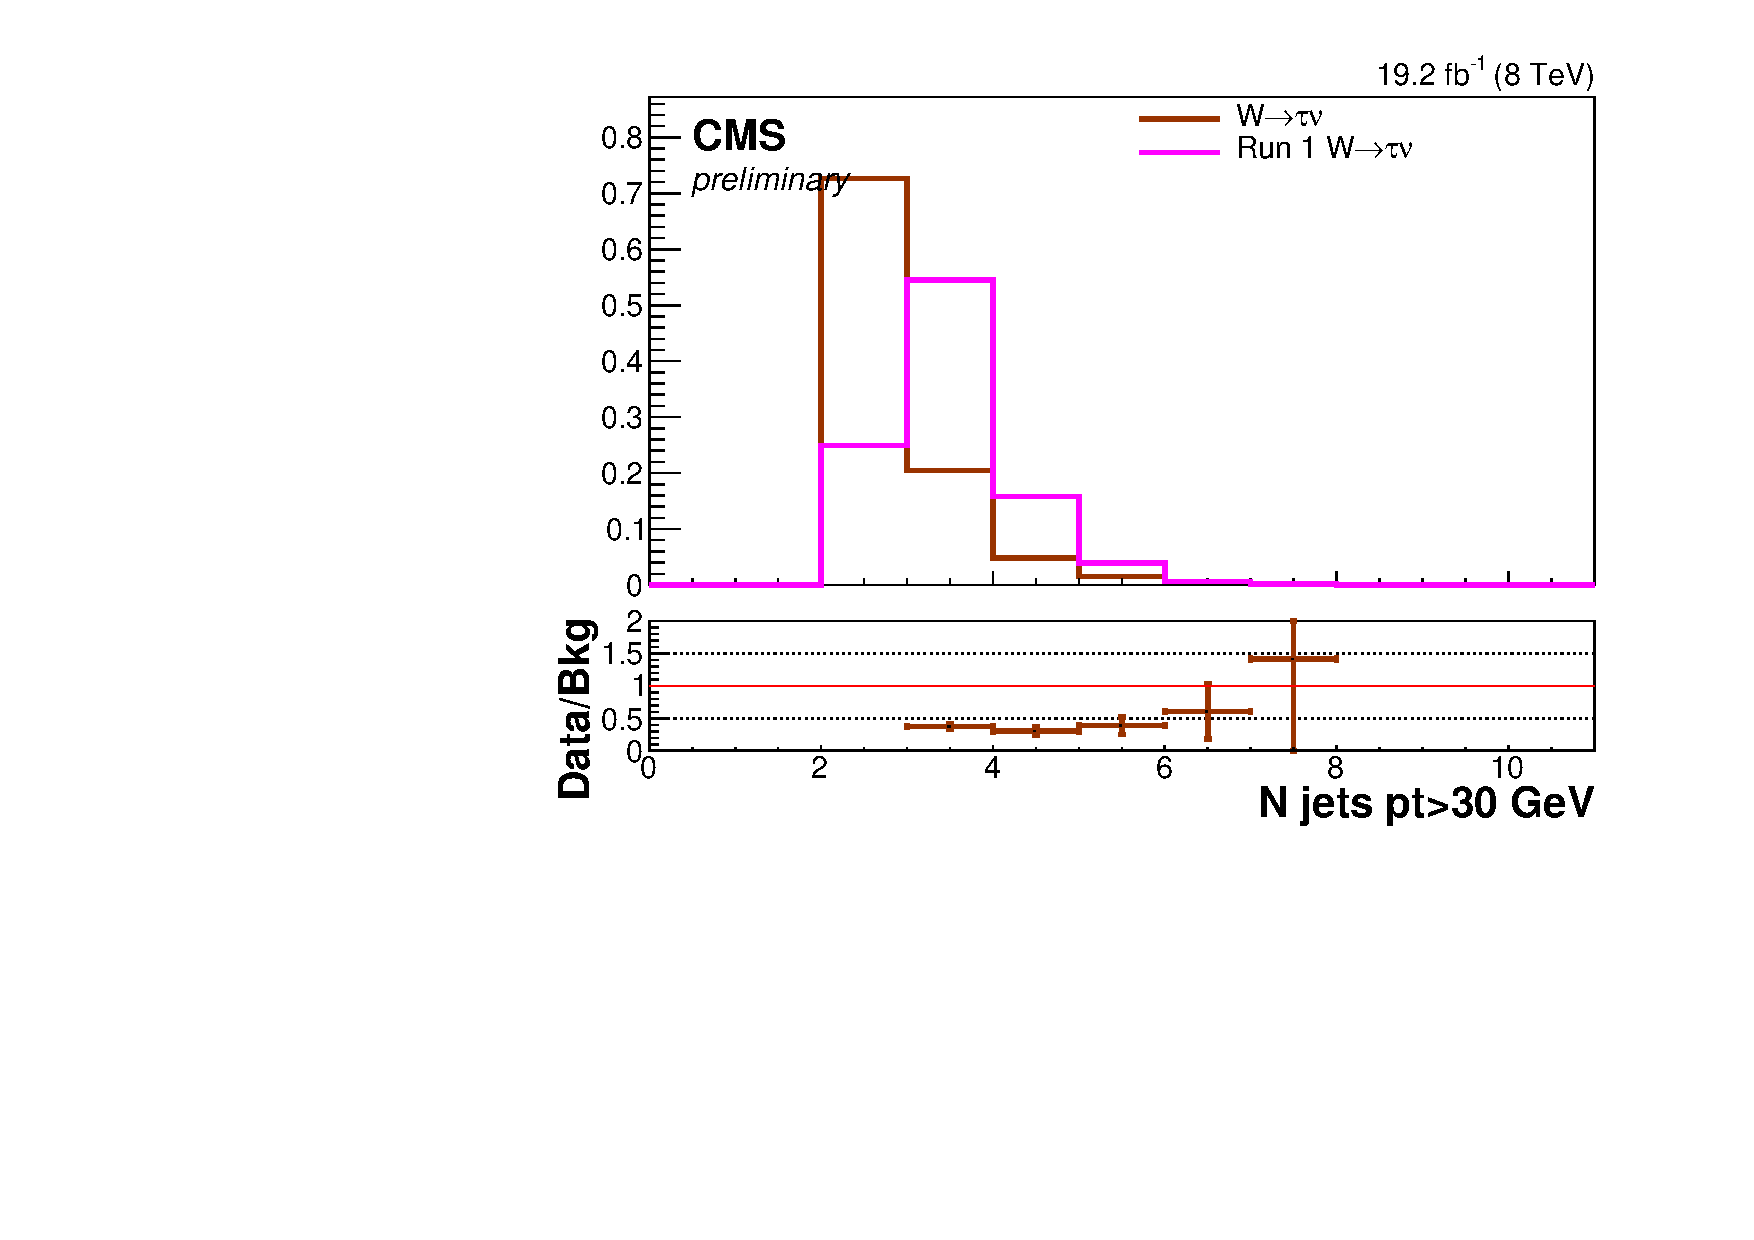
\includegraphics[width=.5\textwidth]{TalkPics/wcontplots090615/output_run1compdynoweight/taunu_norm_n_jets_30.pdf}
  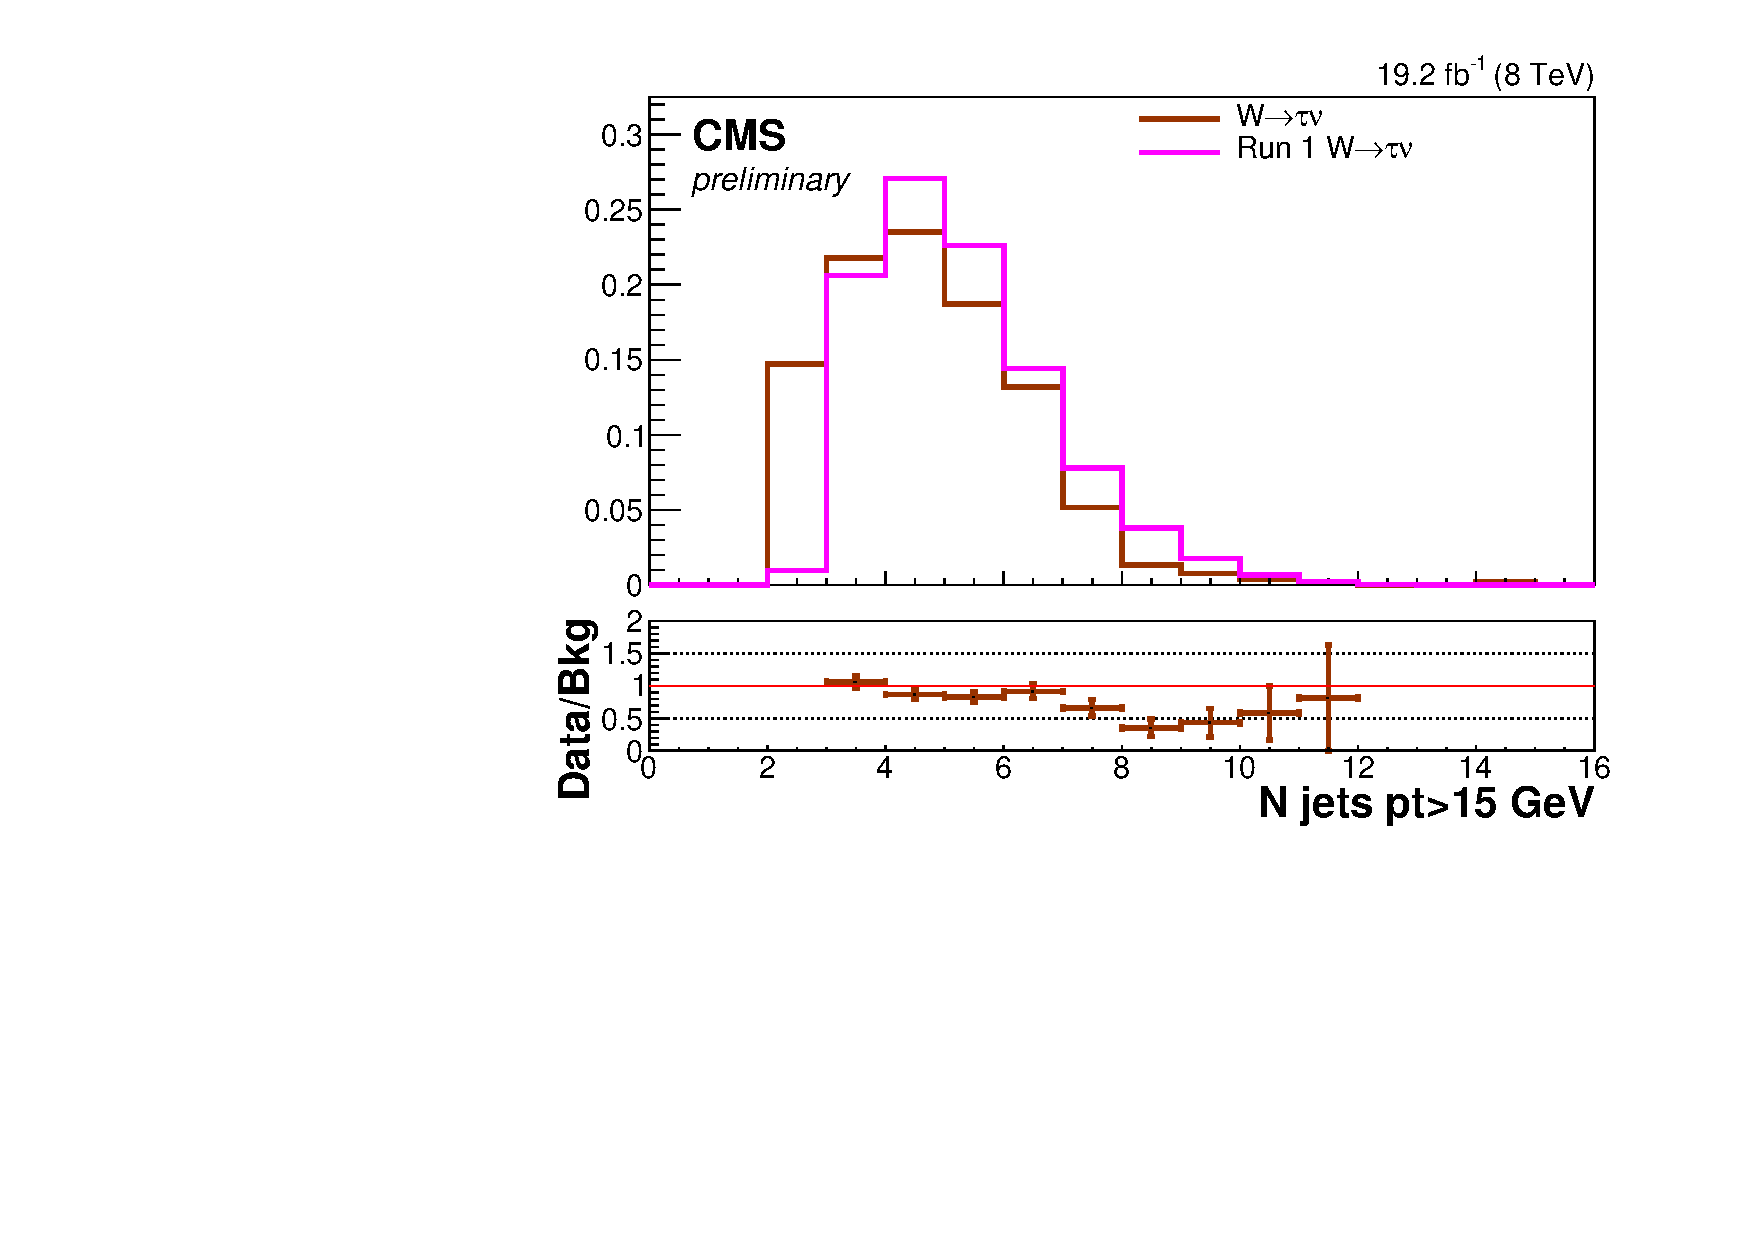
\includegraphics[width=.5\textwidth]{TalkPics/wcontplots090615/output_run1compdynoweight/taunu_norm_n_jets_15.pdf}
\end{frame}

\begin{frame}
  \label{lastframe}
  \begin{block}{Summary}
    \begin{itemize}
      \item W control plots produced
      \item Significant differences seen especially in $p_{T}$ and MET
      \item[-] Could be due to looser cut on MET Sig. due to difference in variable definition from run 1 to run 2
      \item[-] Will reproduce old met significance variable to allow direct comparison
      \item Have installed Scorpion framework for phenomenology work with Bjoern
      \item[-] Next step implement $H\rightarrow inv$ analysis in scorpion
    \end{itemize}
  \end{block}
\end{frame}

\begin{frame}
  \frametitle{Backup}
\end{frame}

\end{fmffile}
\end{document}
